% Options for packages loaded elsewhere
\PassOptionsToPackage{unicode}{hyperref}
\PassOptionsToPackage{hyphens}{url}
%
\documentclass[
]{book}
\usepackage{amsmath,amssymb}
\usepackage{iftex}
\ifPDFTeX
  \usepackage[T1]{fontenc}
  \usepackage[utf8]{inputenc}
  \usepackage{textcomp} % provide euro and other symbols
\else % if luatex or xetex
  \usepackage{unicode-math} % this also loads fontspec
  \defaultfontfeatures{Scale=MatchLowercase}
  \defaultfontfeatures[\rmfamily]{Ligatures=TeX,Scale=1}
\fi
\usepackage{lmodern}
\ifPDFTeX\else
  % xetex/luatex font selection
\fi
% Use upquote if available, for straight quotes in verbatim environments
\IfFileExists{upquote.sty}{\usepackage{upquote}}{}
\IfFileExists{microtype.sty}{% use microtype if available
  \usepackage[]{microtype}
  \UseMicrotypeSet[protrusion]{basicmath} % disable protrusion for tt fonts
}{}
\makeatletter
\@ifundefined{KOMAClassName}{% if non-KOMA class
  \IfFileExists{parskip.sty}{%
    \usepackage{parskip}
  }{% else
    \setlength{\parindent}{0pt}
    \setlength{\parskip}{6pt plus 2pt minus 1pt}}
}{% if KOMA class
  \KOMAoptions{parskip=half}}
\makeatother
\usepackage{xcolor}
\usepackage{color}
\usepackage{fancyvrb}
\newcommand{\VerbBar}{|}
\newcommand{\VERB}{\Verb[commandchars=\\\{\}]}
\DefineVerbatimEnvironment{Highlighting}{Verbatim}{commandchars=\\\{\}}
% Add ',fontsize=\small' for more characters per line
\usepackage{framed}
\definecolor{shadecolor}{RGB}{248,248,248}
\newenvironment{Shaded}{\begin{snugshade}}{\end{snugshade}}
\newcommand{\AlertTok}[1]{\textcolor[rgb]{0.94,0.16,0.16}{#1}}
\newcommand{\AnnotationTok}[1]{\textcolor[rgb]{0.56,0.35,0.01}{\textbf{\textit{#1}}}}
\newcommand{\AttributeTok}[1]{\textcolor[rgb]{0.13,0.29,0.53}{#1}}
\newcommand{\BaseNTok}[1]{\textcolor[rgb]{0.00,0.00,0.81}{#1}}
\newcommand{\BuiltInTok}[1]{#1}
\newcommand{\CharTok}[1]{\textcolor[rgb]{0.31,0.60,0.02}{#1}}
\newcommand{\CommentTok}[1]{\textcolor[rgb]{0.56,0.35,0.01}{\textit{#1}}}
\newcommand{\CommentVarTok}[1]{\textcolor[rgb]{0.56,0.35,0.01}{\textbf{\textit{#1}}}}
\newcommand{\ConstantTok}[1]{\textcolor[rgb]{0.56,0.35,0.01}{#1}}
\newcommand{\ControlFlowTok}[1]{\textcolor[rgb]{0.13,0.29,0.53}{\textbf{#1}}}
\newcommand{\DataTypeTok}[1]{\textcolor[rgb]{0.13,0.29,0.53}{#1}}
\newcommand{\DecValTok}[1]{\textcolor[rgb]{0.00,0.00,0.81}{#1}}
\newcommand{\DocumentationTok}[1]{\textcolor[rgb]{0.56,0.35,0.01}{\textbf{\textit{#1}}}}
\newcommand{\ErrorTok}[1]{\textcolor[rgb]{0.64,0.00,0.00}{\textbf{#1}}}
\newcommand{\ExtensionTok}[1]{#1}
\newcommand{\FloatTok}[1]{\textcolor[rgb]{0.00,0.00,0.81}{#1}}
\newcommand{\FunctionTok}[1]{\textcolor[rgb]{0.13,0.29,0.53}{\textbf{#1}}}
\newcommand{\ImportTok}[1]{#1}
\newcommand{\InformationTok}[1]{\textcolor[rgb]{0.56,0.35,0.01}{\textbf{\textit{#1}}}}
\newcommand{\KeywordTok}[1]{\textcolor[rgb]{0.13,0.29,0.53}{\textbf{#1}}}
\newcommand{\NormalTok}[1]{#1}
\newcommand{\OperatorTok}[1]{\textcolor[rgb]{0.81,0.36,0.00}{\textbf{#1}}}
\newcommand{\OtherTok}[1]{\textcolor[rgb]{0.56,0.35,0.01}{#1}}
\newcommand{\PreprocessorTok}[1]{\textcolor[rgb]{0.56,0.35,0.01}{\textit{#1}}}
\newcommand{\RegionMarkerTok}[1]{#1}
\newcommand{\SpecialCharTok}[1]{\textcolor[rgb]{0.81,0.36,0.00}{\textbf{#1}}}
\newcommand{\SpecialStringTok}[1]{\textcolor[rgb]{0.31,0.60,0.02}{#1}}
\newcommand{\StringTok}[1]{\textcolor[rgb]{0.31,0.60,0.02}{#1}}
\newcommand{\VariableTok}[1]{\textcolor[rgb]{0.00,0.00,0.00}{#1}}
\newcommand{\VerbatimStringTok}[1]{\textcolor[rgb]{0.31,0.60,0.02}{#1}}
\newcommand{\WarningTok}[1]{\textcolor[rgb]{0.56,0.35,0.01}{\textbf{\textit{#1}}}}
\usepackage{longtable,booktabs,array}
\usepackage{calc} % for calculating minipage widths
% Correct order of tables after \paragraph or \subparagraph
\usepackage{etoolbox}
\makeatletter
\patchcmd\longtable{\par}{\if@noskipsec\mbox{}\fi\par}{}{}
\makeatother
% Allow footnotes in longtable head/foot
\IfFileExists{footnotehyper.sty}{\usepackage{footnotehyper}}{\usepackage{footnote}}
\makesavenoteenv{longtable}
\usepackage{graphicx}
\makeatletter
\def\maxwidth{\ifdim\Gin@nat@width>\linewidth\linewidth\else\Gin@nat@width\fi}
\def\maxheight{\ifdim\Gin@nat@height>\textheight\textheight\else\Gin@nat@height\fi}
\makeatother
% Scale images if necessary, so that they will not overflow the page
% margins by default, and it is still possible to overwrite the defaults
% using explicit options in \includegraphics[width, height, ...]{}
\setkeys{Gin}{width=\maxwidth,height=\maxheight,keepaspectratio}
% Set default figure placement to htbp
\makeatletter
\def\fps@figure{htbp}
\makeatother
\setlength{\emergencystretch}{3em} % prevent overfull lines
\providecommand{\tightlist}{%
  \setlength{\itemsep}{0pt}\setlength{\parskip}{0pt}}
\setcounter{secnumdepth}{5}
% definitions for citeproc citations
\NewDocumentCommand\citeproctext{}{}
\NewDocumentCommand\citeproc{mm}{%
  \begingroup\def\citeproctext{#2}\cite{#1}\endgroup}
\makeatletter
 % allow citations to break across lines
 \let\@cite@ofmt\@firstofone
 % avoid brackets around text for \cite:
 \def\@biblabel#1{}
 \def\@cite#1#2{{#1\if@tempswa , #2\fi}}
\makeatother
\newlength{\cslhangindent}
\setlength{\cslhangindent}{1.5em}
\newlength{\csllabelwidth}
\setlength{\csllabelwidth}{3em}
\newenvironment{CSLReferences}[2] % #1 hanging-indent, #2 entry-spacing
 {\begin{list}{}{%
  \setlength{\itemindent}{0pt}
  \setlength{\leftmargin}{0pt}
  \setlength{\parsep}{0pt}
  % turn on hanging indent if param 1 is 1
  \ifodd #1
   \setlength{\leftmargin}{\cslhangindent}
   \setlength{\itemindent}{-1\cslhangindent}
  \fi
  % set entry spacing
  \setlength{\itemsep}{#2\baselineskip}}}
 {\end{list}}
\usepackage{calc}
\newcommand{\CSLBlock}[1]{\hfill\break\parbox[t]{\linewidth}{\strut\ignorespaces#1\strut}}
\newcommand{\CSLLeftMargin}[1]{\parbox[t]{\csllabelwidth}{\strut#1\strut}}
\newcommand{\CSLRightInline}[1]{\parbox[t]{\linewidth - \csllabelwidth}{\strut#1\strut}}
\newcommand{\CSLIndent}[1]{\hspace{\cslhangindent}#1}
\ifLuaTeX
  \usepackage{selnolig}  % disable illegal ligatures
\fi
\usepackage{bookmark}
\IfFileExists{xurl.sty}{\usepackage{xurl}}{} % add URL line breaks if available
\urlstyle{same}
\hypersetup{
  pdftitle={Introduction to Quantitative Text Analysis},
  pdfauthor={Kostas Gemenis and Bastiaan Bruinsma},
  hidelinks,
  pdfcreator={LaTeX via pandoc}}

\title{Introduction to Quantitative Text Analysis}
\author{Kostas Gemenis and Bastiaan Bruinsma}
\date{}

\begin{document}
\maketitle

{
\setcounter{tocdepth}{1}
\tableofcontents
}
\chapter*{Welcome!}\label{welcome}
\addcontentsline{toc}{chapter}{Welcome!}

Welcome to our introductory textbook on quantitative text analysis! This book originated as a collection of assignments and lecture slides that we prepared for the ECPR Winter and Summer Schools in Methods and Techniques. Later, as we taught the Introduction to Quantitative Analysis course at the ECPR Schools, the MethodsNET Summer School, and seminars at the Max Planck Institute for the Study of Societies, Goethe University Frankfurt, Chalmers University, and the Cyprus University of Technology, we added more and more material and text, resulting in this book. The version you see today has been updated with the help of a grant from the {[}Learning Development Network{]} (\url{https://ldn.cut.ac.cy/}) at the Cyprus University of Technology. For now, the book focuses on some of the best-known quantitative text analysis methods in the field, showing what they are and how to run them in R.

So why bother with quantitative content analysis? For one thing, we can say that developments over the last twenty years have made research using quantitative text analysis a particularly exciting proposition. First, the huge increase in computing power has made it possible to work with large amounts of text. Second, there is the development of R - a free, open-source, cross-platform statistical software. This development has enabled many researchers and programmers to develop packages for statistical methods for working with text. In addition, the spread of the internet has made many interesting sources of textual data available in digital form. Add to this the emergence of social media as a massive source of text generated daily by millions of users around the world.

However, quantitative text analysis can be a daunting experience for someone unfamiliar with quantitative methods or programming. Our aim with this book is to guide you through it, combining theoretical explanations with a step-by-step explanation of the code. There are also several exercises designed for those with little or no experience in text analysis, R, or quantitative methods. Ultimately, we hope that you will find this book not only informative but also engaging and educational.

\chapter{Getting Started with Quantitative Text Analysis}\label{getting-started-with-qta}

Quantitative text analysis, like many other techniques, is at its core a method. This means that while it provides you with the tools to answer a particular question, it does not provide you with a theoretical framework. Nor is there any reality to be discovered: the only thing we can do with QTA methods is to provide (hopefully) accurate summaries of our texts.

With this in mind, there are five questions that we can hope to answer with QTA (\citeproc{ref-Grimmer2022a}{Grimmer et al., 2022}):

\begin{enumerate}
\def\labelenumi{\arabic{enumi}.}
\tightlist
\item
  What do our texts look like?
\item
  What are our texts about?
\item
  What do our texts measure?
\item
  What can our texts predict?
\item
  What can our texts prove?
\end{enumerate}

In the case of the first question, we might simply be interested in how many words we have in different documents, which authors wrote together, or whether certain texts have a distinctive type of wording. Questions like these help us to get a better idea of the type of data we are dealing with, to work out what might be interesting to look at and to identify potential problems early on. We can then ask ourselves what the texts are actually about. Here we could run topic models to look at (a representation of) the underlying structure of our texts. We could look at the sentiment of the texts using different dictionaries, or calculate different readability statistics. In each case, we get a better understanding of what our texts represent and what they might be about. For example, we might discover that some texts cluster together unexpectedly, or have more themes in common than we expected. This might then lead us to focus on them exclusively, to collect more texts on the same topic, or to focus on different documents altogether.

Now that we have our texts and know what we want from them, we can start to use them to measure a concept we are interested in. For example, we could use the codes from the \href{https://manifesto-project.wzb.eu/}{Manifesto Project} to measure the political left-right position of our texts. Or we could measure the occurrence of different issues in these documents to find out the agendas of different parties. Once this is done, we could then use these measurements to predict what kind of agenda a new party might have, or a step further, we could use them to estimate what effect a particular text will have on, say, voters or legislators.

Note that we can stop this process and any point and do interesting work. That is, if we go about rigorously collecting texts from different sources, structuring them, cleaning them, and describing what they are like, this can be interesting in itself. Similarly, measuring the positions of texts on a variety of scales can be enough to make for interesting research. Ultimately, how far you go depends on the questions you want to ask and the problems you want to solve.

\section{QTA in steps}\label{qta-in-steps}

So what does a QTA look like in practice? Let's say you already have an idea of what you want to do and what questions you want to ask. Then you need to go through the following steps:

\begin{enumerate}
\def\labelenumi{\arabic{enumi}.}
\item
  \textbf{Choose and select}. If you want to look at political manifestos, do you want to see all of them or just those of the major parties? And do you want only the most recent ones or all of them?
\item
  \textbf{Find and collect}. Find all the texts you need and save them somewhere. Make sure that everything you want is included, that you have the right version of the document and that the documents are in a readable format (pdf, txt or .doc format).
\item
  \textbf{Check}. If your documents are in .txt format, are there any conversion errors? For example, is a letter like ``Ü'' visible in the document, or do you see something like ``™'' instead? Note that most researchers work in English, and non-English and non-Latin alphabets can cause problems. The best option is to ensure that all your documents are in UTF-8 (more on this here).
\item
  \textbf{Create a corpus}. Load all the texts you want to analyse and associate them with any metadata you want to include. Then transform the texts into a data frequency matrix (DFM). This matrix has your individual texts in the rows and all possible words in the columns - this turns your corpus of textual data into a matrix of numbers.
\item
  \textbf{Preprocess}. Remove words you do not need, such as stop words, remove punctuation, and apply stemming or lemmatisation algorithms.
\item
  \textbf{Describe}. Check your data. Are there any words that occur a lot (and which you might want to remove?) Are there any strange patterns? Is the data in the right form?
\item
  \textbf{Run your model}. Select your model, run it and check that all the hyperparameter settings are correct. Check that all the steps are correct and repeat the process at least once to ensure future reproducibility.
\end{enumerate}

Visualise and interpret. Look at your results using tables and graphs and try to see if you can answer your research question.

Of all these steps, you will often find that the last two are the most commonly covered. However, it is equally important to ensure that your data is correct and of sufficient quality to be of real use. Often problems later in the analysis are caused by problems in the data early on.

\section{How this book works}\label{how-this-book-works}

From here on, this book will work as follows. In @ref(getting-started-with-r) we will look at R and how to get it working on our system. Our choice of R here is based on the fact that it is both open and free, as well as being the current choice of software for most social scientists (and therefore the one you are most likely to be working with). R also has a wide range of packages that we can use for text analysis. Then in @ref(\#importing-data), we will focus on the actual texts we are going to use and how to get them into R. This will cover converting PDF files to TXT, reading CSV files, and downloading files from an on-line database. Then in @ref(reliability-validity), we will cover the outstanding issues of reliability and validity, and how to ensure that the codes you get from (a more classical) text analysis are reliable enough to use later. Then, in @ref(\#preliminaries), we look at what is in our data and how we can best describe the texts we are dealing with. Finally, the last four chapters cover the four main types of techniques we can use to find out more about our text or measure things about it: @ref(dictionary-analysis), @ref(scaling), @ref(supervised-methods) and @ref(unsupervised-methods). We conclude, of course, with a list of references that we have used and that you can use if you are interested in learning more.

\section{Further Literature}\label{further-literature}

There has been no shortage recently of good introductions to content analysis. Which book would be best for you depends therefore mostly on your focus. For a traditional (more qualitative) introduction, ``Content Analysis - an Introduction to Its Methodology'' by Klaus Krippendorff (currently in its 4th edition) is a good place to start. For a more quantitative approach, ``Text as Data: A New Framework for Machine Learning and the Social Sciences'' by Grimmer, Roberts and Stewart from 2022, is the latest in combining machine learning with text analysis. Finally, for another qualitative approach, ``The Content Analysis Guidebook'' by Kimberly Neuendorf (currently in its 2nd edition) delves deeper into the underlying theory (which we cursorily discuss here).

\chapter{Getting Started with R}\label{getting-started-with-r}

Over the last few years, two approaches have emerged to deal with issues related to the quantitative analysis of text: R and Python. While Python is a general-purpose language (useful for everything from websites to games to databases), R was always designed with statistics in mind. As a result, R is better suited to deep statistical analysis and a wide range of data visualisation. As a result, while Python is a good choice when dealing with issues related to machine learning and large-scale applications, R is better suited to statistical learning and data exploration. Since we are mainly interested in the latter here, we built this book around R (and all the packages it offers). If you are more interested in large-scale analysis using Python, be sure to take a look at its \href{https://spacy.io}{spaCy} and \href{https://www.nltk.org}{NLTK} libraries.

\section{What is R?}\label{what-is-r}

R is an open-source program that allows you to perform a wide variety of statistical tasks. At its core, it is a modification of the S and Scheme programming languages, making it not only flexible but also fast. R is available for Windows, Linux and OS X, and is updated regularly. In its basic form, R uses a simple command line interface. To make it more friendly, you can use one of the integrated development environments (IDEs) such as \href{https://www.rstudio.com/}{RStudio}, \href{https://jupyter.org/}{Jupyter} and \href{https://socialsciences.mcmaster.ca/jfox/Misc/Rcmdr/}{R Commander}. These environments not only look better but also offer some additional practical features. In this book, we will use RStudio as it is (in our opinion) the best-looking and working IDE available.

\section{R on Windows}\label{r-on-windows}

To install R on Windows, go to \url{https://cran.r-project.org/bin/windows/base/}, download the file, double-click it and run it. During installation, it is best to leave default options (such as the installation folder) unchanged. This makes it easier for other programs to know where to find R. Once installed, you will find two shortcuts for R on your desktop. These refer to the two versions of R that come with the installation - the 32-bit version and the 64-bit version. Which version you need will depend on your version of Windows. To find out which version of Windows you have, go to \textbf{This PC} (or \textbf{My Computer}), right-click and select \textbf{Properties}. Here you should find the version of Windows installed on your PC. If you have a 64-bit version of Windows, you can use either version. However, it is best to use the 64-bit version as it makes better use of your computer's memory and runs more smoothly. If you have the 32-bit version of Windows, you must use the 32-bit version of R.

To install RStudio, go to \url{https://www.rstudio.com/products/rstudio/download/} and download the free version of RStudio at the bottom of the page. Make sure you select \textbf{Installers for Supported Platforms} and select the option for Windows. Once downloaded, install the program leaving all settings unchanged. If all goes well, RStudio will have found your installation of R and placed a shortcut on your desktop. Whether you have a 32-bit or 64-bit version of Windows or R does not matter to RStudio. What does matter are the slashes. R uses slashes (\texttt{/}) instead of the backslashes (\texttt{\textbackslash{}}) that Windows uses. So whenever you refer to a folder or file in R, make sure you reverse the slashes. For example, you should refer to a file that has the Windows address \textbf{C:\textbackslash Users\textbackslash Desktop\textbackslash data.csv} as \textbf{C:/Users/Desktop/data.csv}.

\section{R on Linux}\label{r-on-linux}

How you install R on Linux depends on which flavour of Linux you have. In most cases, R is already included in your Linux distribution. You can check this by opening a terminal and typing \texttt{R}. If it is installed, R will start in the terminal. If R is not part of your system, run the following in a terminal

\begin{enumerate}
\def\labelenumi{\arabic{enumi}.}
\tightlist
\item
  sudo apt update
\item
  sudo apt install r-base r-base-dev -y
\item
  Now run ``R'' to see if the installation worked
\end{enumerate}

To install RStudio, go to \url{https://www.rstudio.com/products/rstudio/download/}. At the bottom of the page, select the installer for your operating system. Then install the file either using an installation manager or via the terminal. After running the launcher, you will find RStudio in the Dash.

\section{R on MacOS}\label{r-on-macos}

For OS X, you must have OS X 10.6 (Snow Leopard) or later. Otherwise, you can still install R, but you will not be able to use a certain number of packages (like some we use here). To check this, click on the Apple icon at the top left of your screen. Then click on the \textbf{About This Mac} option. A window should appear telling you which version of OS X (or MacOS) you have.

To install R, go to \url{https://cran.r-project.org/index.html} and click on \textbf{Download R for (Mac) OS X}. Once there, download and install the appropriate .pkg file for your version of OS X. You will also need to download the \textbf{Clang 6.x Compiler} and the \textbf{GNU Fortran Compiler} from \url{https://cran.r-project.org/bin/macosx/tools/}. Install both, leaving the selected options as they are. Once installed, check that R works by running it.

To install RStudio, go to \url{https://www.rstudio.com/products/rstudio/download/} and download the OSX version at the bottom of the page. Once downloaded and installed, you should be able to find RStudio among your other applications.

\section{R in the Cloud}\label{r-in-the-cloud}

As well as installing R on your system, you can also use the cloud version. RStudio hosts this version at \url{https://posit.cloud/}. To use it, go to the Sign-Up button at the top right of the screen. Then select the \textbf{Cloud Free} option and select Sign-Up again. Finish the process by either filling in your details or connecting to your Google or GitHub account. Once done, log in and you will be taken to your workspace. To get started, you will need to create a new project. To do this, click on the \textbf{New Project} button, which will take you to an instance of RStudio. From here on, the program works in exactly the same way as the desktop version. Note that anything you do - or packages you install - in the project will remain in the project. So if you want to create a new project, you will have to reinstall it. Also, note that Posit Cloud is highly dependent on both the number of users on the server and your internet connection. Therefore, some actions (such as installing packages) may take longer to complete.

\chapter{Installing Packages}\label{installing-packages}

R on its own is a pretty bare-bones experience. What makes it work are the many packages that exist for it. These packages come in two types: those with an official release and those in development.

\section{Installing from CRAN}\label{installing-from-cran}

For an official release, the package must be part of CRAN: the \emph{Comprehensive R Archive Network}.CRAN is a website that collects and hosts all the material R needs, such as the various distributions, packages and more. The main advantage of being official is that it means the package has been through a review process. This ensures that the package is free of major bugs, has README and NEWS files, and has a unique version number. In addition, packages that have been officially released often have accompanying articles in \href{https://www.https://journal.r-project.org/}{\emph{The R Journal}} or \href{https://www.jstatsoft.org/index}{\emph{The Journal of Statistical Software}} that provide detailed explanations of the code, examples, etc.

To install official packages, we can use the \texttt{install.packages\textquotesingle{}\ command\ or\ the\ **Packages**\ tab\ in\ RStudio.\ If\ we\ run}install.packages(``package'', dependencies=TRUE)\texttt{,\ we\ will\ also\ install\ any\ other\ packages\ a\ package\ depends\ on.\ Finally,\ to\ update,\ we\ can\ either\ go\ to\ the\ **Packages**\ tab\ in\ RStudio\ and\ click\ the\ **Update**\ button.\ We\ can\ also\ type}update.packages()` in the \textbf{Console } for the same result. Try to update your package often to avoid unnecessary bugs and problems.

\section{Installing from GitHub}\label{installing-from-github}

Some packages that have not yet had an official release are in development on \href{https://github.com/}{\textbf{GitHub}}. As a result, these packages change very often and are more unstable than their official counterparts. We can install packages from Github using the \texttt{devtools} package. To install this, type:

\begin{Shaded}
\begin{Highlighting}[]
\FunctionTok{install.packages}\NormalTok{(}\StringTok{"devtools"}\NormalTok{, }\AttributeTok{dependencies=}\ConstantTok{TRUE}\NormalTok{)}
\end{Highlighting}
\end{Shaded}

Here, \texttt{dependencies=TRUE} ensures that if we need other packages to make \texttt{devtools} work, R will install these as well. Depending on your operating system, you might have to install some other software for \texttt{devtools} to work.

On Windows, \texttt{devtools} requires the \textbf{RTools} software. To install this, go to \url{https://cran.r-project.org/bin/windows/Rtools/}, download the latest \textbf{recommended} version (in green), and install it. Then re-open R again and install \texttt{devtools} as shown above.

On Linux, the way you install \texttt{devtools} depends on the flavour of Linux you have. In most cases, installing `devtools' from the RStudio console will work fine. If not, the problem is most likely a missing package in your Linux distribution. To fix this, close R, open a terminal and type:

\begin{enumerate}
\def\labelenumi{\arabic{enumi}.}
\tightlist
\item
  \texttt{sudo\ apt-get\ update}
\item
  \texttt{sudo\ apt-get\ upgrade}
\item
  \texttt{sudo\ apt\ install\ build-essential\ libcurl4-gnutls-dev\ libxml2-dev\ libssl-dev}
\item
  Close the terminal, open R, and install \texttt{devtools} as shown above.
\end{enumerate}

On OSX (or macOS), \texttt{devtools} requires the \emph{XCode} software. To install this, follow these steps:

\begin{enumerate}
\def\labelenumi{\arabic{enumi}.}
\tightlist
\item
  Launch the terminal (which you can find in \emph{/Applications/Utilities/}), and type:
\item
  In the terminal, type: \texttt{xcode-select\ -\/-install}
\item
  A software update window should pop up. Here, click \textbf{Install} and agree to the Terms of Service.
\item
  Go to R and install \texttt{devtools} as shown above.
\end{enumerate}

\section{Packages for Quantitative Text Analysis in R}\label{packages-for-quantitative-text-analysis-in-r}

There are several packages that we can use for quantitative text analysis in R, such as \texttt{tm}, \texttt{tidytext}, \texttt{RTextTools}, \texttt{corpus} and \texttt{koRpus} (\citeproc{ref-Welbers2017a}{Welbers et al., 2017}). Many of these packages offer specialised features that can sometimes be very useful, but in this book, we will mainly rely on \texttt{quanteda} (\citeproc{ref-Benoit2018a}{Benoit et al., 2018}), which is currently in its fourth version. The advantage of \texttt{quanteda} over other packages is that it integrates into a common framework many of the text analysis functions of R that were previously spread across many different packages(\citeproc{ref-Welbers2017a}{Welbers et al., 2017}).In addition, many `quanteda' functions can be easily combined with functions in other packages, while the package as a whole has simple and logical commands and a well-maintained \href{www.quanteda.io}{website}.

The current version of \texttt{quanteda} at the time of writing is 4.0. This version works best with R version 4.0.1 or higher. To check if your system has this, type \texttt{R.Version()} in your console. The result will be a list. Look for \texttt{\$version.string} to see what version number your version of R is. If you do not have the latest version, see the steps above to install the latest version.

To install \texttt{quanteda}, type:

\begin{Shaded}
\begin{Highlighting}[]
\FunctionTok{install.packages}\NormalTok{(}\StringTok{"quanteda"}\NormalTok{, }\AttributeTok{dependencies =} \ConstantTok{TRUE}\NormalTok{)}
\end{Highlighting}
\end{Shaded}

Note that because we wrote \texttt{dependencies\ =\ TRUE}, this command also installed three other \texttt{quanteda} helper packages, which serve to extend the basic tools that are already inside \texttt{quanteda}. In the future, more of these helper packages can be expected to extend the main \texttt{quanteda} package even further. However, before these helper packages get an official release, we can already find them in development on GitHub.In this book, we will install two of them - \texttt{quanteda.classifiers}, which we will use for supervised learning methods, and \texttt{quanteda.dictionaries}, which we will use for dictionary analysis:

\begin{Shaded}
\begin{Highlighting}[]
\FunctionTok{library}\NormalTok{(devtools)}
\FunctionTok{install\_github}\NormalTok{(}\StringTok{"quanteda/quanteda.classifiers"}\NormalTok{, }\AttributeTok{dependencies =} \ConstantTok{TRUE}\NormalTok{)}
\FunctionTok{install\_github}\NormalTok{(}\StringTok{"kbenoit/quanteda.dictionaries"}\NormalTok{, }\AttributeTok{dependencies =} \ConstantTok{TRUE}\NormalTok{)}
\FunctionTok{install\_github}\NormalTok{(}\StringTok{"quanteda/quanteda.corpora"}\NormalTok{, }\AttributeTok{dependencies =} \ConstantTok{TRUE}\NormalTok{)}
\end{Highlighting}
\end{Shaded}

In addition to \texttt{quanteda} we then use the following packages:

\begin{Shaded}
\begin{Highlighting}[]
\FunctionTok{install\_github}\NormalTok{(}\StringTok{"mikegruz/kripp.boot"}\NormalTok{, }\AttributeTok{dependencies =} \ConstantTok{TRUE}\NormalTok{)}
\FunctionTok{install.packages}\NormalTok{(}\StringTok{"ca"}\NormalTok{, }\AttributeTok{dependencies =} \ConstantTok{TRUE}\NormalTok{)}
\FunctionTok{install.packages}\NormalTok{(}\StringTok{"combinat"}\NormalTok{, }\AttributeTok{dependencies =} \ConstantTok{TRUE}\NormalTok{)}
\FunctionTok{install.packages}\NormalTok{(}\StringTok{"DescTools"}\NormalTok{, }\AttributeTok{dependencies =} \ConstantTok{TRUE}\NormalTok{)}
\FunctionTok{install.packages}\NormalTok{(}\StringTok{"FactoMineR"}\NormalTok{, }\AttributeTok{dependencies =} \ConstantTok{TRUE}\NormalTok{)}
\FunctionTok{install.packages}\NormalTok{(}\StringTok{"factoextra"}\NormalTok{, }\AttributeTok{dependencies =} \ConstantTok{TRUE}\NormalTok{)}
\FunctionTok{install.packages}\NormalTok{(}\StringTok{"Factoshiny"}\NormalTok{, }\AttributeTok{dependencies =} \ConstantTok{TRUE}\NormalTok{)}
\FunctionTok{install.packages}\NormalTok{(}\StringTok{"Hmisc"}\NormalTok{, }\AttributeTok{dependencies =} \ConstantTok{TRUE}\NormalTok{)}
\FunctionTok{install.packages}\NormalTok{(}\StringTok{"httr"}\NormalTok{, }\AttributeTok{dependencies =} \ConstantTok{TRUE}\NormalTok{)}
\FunctionTok{install.packages}\NormalTok{(}\StringTok{"jsonlite"}\NormalTok{, }\AttributeTok{dependencies =} \ConstantTok{TRUE}\NormalTok{)}
\FunctionTok{install.packages}\NormalTok{(}\StringTok{"manifestoR"}\NormalTok{, }\AttributeTok{dependencies =} \ConstantTok{TRUE}\NormalTok{)}
\FunctionTok{install.packages}\NormalTok{(}\StringTok{"readr"}\NormalTok{, }\AttributeTok{dependencies =} \ConstantTok{TRUE}\NormalTok{)}
\FunctionTok{install.packages}\NormalTok{(}\StringTok{"readtext"}\NormalTok{, }\AttributeTok{dependencies =} \ConstantTok{TRUE}\NormalTok{)}
\FunctionTok{install.packages}\NormalTok{(}\StringTok{"reshape2"}\NormalTok{, }\AttributeTok{dependencies =} \ConstantTok{TRUE}\NormalTok{)}
\FunctionTok{install.packages}\NormalTok{(}\StringTok{"RTextTools"}\NormalTok{, }\AttributeTok{dependencies =} \ConstantTok{TRUE}\NormalTok{)}
\FunctionTok{install.packages}\NormalTok{(}\StringTok{"R.temis"}\NormalTok{, }\AttributeTok{dependencies =} \ConstantTok{TRUE}\NormalTok{)}
\FunctionTok{install.packages}\NormalTok{(}\StringTok{"rvest"}\NormalTok{, }\AttributeTok{dependencies =} \ConstantTok{TRUE}\NormalTok{)}
\FunctionTok{install.packages}\NormalTok{(}\StringTok{"seededlda"}\NormalTok{, }\AttributeTok{dependencies =} \ConstantTok{TRUE}\NormalTok{)}
\FunctionTok{install.packages}\NormalTok{(}\StringTok{"stm"}\NormalTok{, }\AttributeTok{dependencies =} \ConstantTok{TRUE}\NormalTok{)}
\FunctionTok{install.packages}\NormalTok{(}\StringTok{"tidyverse"}\NormalTok{, }\AttributeTok{dependencies =} \ConstantTok{TRUE}\NormalTok{)}
\FunctionTok{install.packages}\NormalTok{(}\StringTok{"topicmodels"}\NormalTok{, }\AttributeTok{dependencies =} \ConstantTok{TRUE}\NormalTok{)}
\FunctionTok{install.packages}\NormalTok{(}\StringTok{"magick"}\NormalTok{, }\AttributeTok{dependencies =} \ConstantTok{TRUE}\NormalTok{)}
\FunctionTok{install.packages}\NormalTok{(}\StringTok{"vader"}\NormalTok{, }\AttributeTok{dependencies =} \ConstantTok{TRUE}\NormalTok{)}
\end{Highlighting}
\end{Shaded}

Some of these are specialised packages for text analysis, others for statistical estimation and visualisation. After installation, you will find these packages, as well as the \texttt{quanteda} and \texttt{devtools} packages, under the \textbf{Packages} tab in RStudio.

\section{Problems, Bugs and Errors}\label{problems-bugs-and-errors}

It is not uncommon to get errors when typing a command in R. Errors often occur when you misspell the code or use the wrong code for the job at hand. In these cases, R will print a message (in red) telling you why it cannot do what you want it to do. Sometimes this message is quite clear, like telling you to install an extra package. Other times it is more complicated and requires some extra work. In these cases, there are four questions you should ask yourself:

\begin{enumerate}
\def\labelenumi{\arabic{enumi}.}
\tightlist
\item
  Have I downloaded all the packages I need?
\item
  Are all my packages up to date?
\item
  Did I spell the commands correctly?
\item
  Is the data in the correct form or format?
\end{enumerate}

If none of these provide a solution, you can always look online to see if others have encountered the same problem. Often, copying and pasting your error into a search engine will give you other examples, and usually a solution. A well-known place for solutions is \href{https://stackoverflow.com/}{Stack Overflow}, where you can share your problem with others and see if someone can offer a solution. However, make sure you read through the problems that have already been posted to make sure you do not post the same problem twice. We have also compiled a list of problems encountered by people who have used this book, along with their solutions, in this spreadsheet.

\chapter{Importing Data}\label{importing-data}

Before we can do any kind of analysis, we need to get our text into R. Here we look at five different ways of doing this: a) using .txt files, b) using .pdf files, c) using .csv files, d) using an API, and e) using web scraping techniques. Before we do that, though, let us first look at how R looks at text in the first place, and what some of the most basic things we can do with text there are.

\section{Text in R}\label{text-in-r}

R sees any form of text as a vector consisting of different types of characters. In their simplest form, these vectors only have a single character in them. At their most complicated, they can contain many sentences or even whole stories. To see how many characters a vector has, we can use the \texttt{nchar} function:

\begin{Shaded}
\begin{Highlighting}[]
\NormalTok{vector1 }\OtherTok{\textless{}{-}} \StringTok{"This is the first of our character vectors"}
\FunctionTok{nchar}\NormalTok{(vector1)}
\end{Highlighting}
\end{Shaded}

\begin{verbatim}
## [1] 42
\end{verbatim}

\begin{Shaded}
\begin{Highlighting}[]
\FunctionTok{length}\NormalTok{(vector1)}
\end{Highlighting}
\end{Shaded}

\begin{verbatim}
## [1] 1
\end{verbatim}

This example also shows the logic of R. First, we assign the text we have to a certain object. We do so using the \texttt{\textless{}-} arrow. This arrow points from the text we have to the object R stores it in, which we here call \texttt{vector1}. We then ask R to give us the number of characters inside this object, which is 40 in this case. The \texttt{length} command returns something else, namely 1. This means that we have a single sentence, or word, in our object. If we want to, we can place more sentences inside our object using the \texttt{c()} option:

\begin{Shaded}
\begin{Highlighting}[]
\NormalTok{vector2 }\OtherTok{\textless{}{-}} \FunctionTok{c}\NormalTok{(}\StringTok{"This is an example"}\NormalTok{, }\StringTok{"This is another"}\NormalTok{, }\StringTok{"And so we can go on."}\NormalTok{)}
\FunctionTok{length}\NormalTok{(vector2)}
\end{Highlighting}
\end{Shaded}

\begin{verbatim}
## [1] 3
\end{verbatim}

\begin{Shaded}
\begin{Highlighting}[]
\FunctionTok{nchar}\NormalTok{(vector2)}
\end{Highlighting}
\end{Shaded}

\begin{verbatim}
## [1] 18 15 20
\end{verbatim}

\begin{Shaded}
\begin{Highlighting}[]
\FunctionTok{sum}\NormalTok{(}\FunctionTok{nchar}\NormalTok{(vector2))}
\end{Highlighting}
\end{Shaded}

\begin{verbatim}
## [1] 53
\end{verbatim}

Another thing we can do is extract certain words from a sentence. For this, we use the \texttt{substr()} function. With this function, R gives us all the characters that occur between two specific positions. So, when we want the characters between the 4th and 10th characters, we write:

\begin{Shaded}
\begin{Highlighting}[]
\NormalTok{vector3 }\OtherTok{\textless{}{-}} \StringTok{"This is yet another sentence"}
\FunctionTok{substr}\NormalTok{(vector3, }\DecValTok{4}\NormalTok{, }\DecValTok{10}\NormalTok{)}
\end{Highlighting}
\end{Shaded}

\begin{verbatim}
## [1] "s is ye"
\end{verbatim}

We can also split a character vector into smaller parts. We often do this when we want to split a longer text into several sentences. To do so, we use the \texttt{strsplit} function:

\begin{Shaded}
\begin{Highlighting}[]
\NormalTok{vector3 }\OtherTok{\textless{}{-}} \StringTok{"Here is a sentence {-} And a second"}
\NormalTok{parts1 }\OtherTok{\textless{}{-}} \FunctionTok{strsplit}\NormalTok{(vector3, }\StringTok{"{-}"}\NormalTok{)}
\NormalTok{parts1}
\end{Highlighting}
\end{Shaded}

\begin{verbatim}
## [[1]]
## [1] "Here is a sentence " " And a second"
\end{verbatim}

If we now look in the Environment window, we will see that R calls \texttt{parts1} a list. This is another type of object that R uses to store information. We will see it more often later on. For now, it is good to remember that lists in R can have many vectors (the layers of the list) and that in each of these vectors we can store many objects. Here, our list has only a single vector. To create a longer list, we have to add more vectors, and then join them together, again using the \texttt{c()} command:

\begin{Shaded}
\begin{Highlighting}[]
\NormalTok{vector4 }\OtherTok{\textless{}{-}} \StringTok{"Here is another sentence {-} And one more"}
\NormalTok{parts2 }\OtherTok{\textless{}{-}} \FunctionTok{strsplit}\NormalTok{(vector4, }\StringTok{"{-}"}\NormalTok{)}
\NormalTok{parts3 }\OtherTok{\textless{}{-}} \FunctionTok{c}\NormalTok{(parts1, parts2)}
\end{Highlighting}
\end{Shaded}

We can now look at this new list in the Environment and check that it indeed has two elements. A further thing we can do is to join many vectors together. For this, we can use the \texttt{paste} function. Here, the \texttt{sep} argument defines how R will combine the elements:

\begin{Shaded}
\begin{Highlighting}[]
\NormalTok{fruits }\OtherTok{\textless{}{-}} \FunctionTok{paste}\NormalTok{(}\StringTok{"oranges"}\NormalTok{, }\StringTok{"lemons"}\NormalTok{, }\StringTok{"pears"}\NormalTok{, }\AttributeTok{sep =} \StringTok{"{-}"}\NormalTok{)}
\NormalTok{fruits}
\end{Highlighting}
\end{Shaded}

\begin{verbatim}
## [1] "oranges-lemons-pears"
\end{verbatim}

Note that we can also use this command that pastes objects that we made earlier together. For example:

\begin{Shaded}
\begin{Highlighting}[]
\NormalTok{sentences }\OtherTok{\textless{}{-}} \FunctionTok{paste}\NormalTok{(vector3, vector4, }\AttributeTok{sep =} \StringTok{"."}\NormalTok{)}
\NormalTok{sentences}
\end{Highlighting}
\end{Shaded}

\begin{verbatim}
## [1] "Here is a sentence - And a second.Here is another sentence - And one more"
\end{verbatim}

Finally, we can change the case (lowercase, uppercase) of the sentence. To do this, we can use \texttt{tolower} and \texttt{toupper}:

\begin{Shaded}
\begin{Highlighting}[]
\FunctionTok{tolower}\NormalTok{(sentences)}
\end{Highlighting}
\end{Shaded}

\begin{verbatim}
## [1] "here is a sentence - and a second.here is another sentence - and one more"
\end{verbatim}

\begin{Shaded}
\begin{Highlighting}[]
\FunctionTok{toupper}\NormalTok{(sentences)}
\end{Highlighting}
\end{Shaded}

\begin{verbatim}
## [1] "HERE IS A SENTENCE - AND A SECOND.HERE IS ANOTHER SENTENCE - AND ONE MORE"
\end{verbatim}

Again, we can also run the same command when we have more than a single element in our vector:

\begin{Shaded}
\begin{Highlighting}[]
\NormalTok{sentences2 }\OtherTok{\textless{}{-}} \FunctionTok{c}\NormalTok{(}\StringTok{"This is a piece of example text"}\NormalTok{, }\StringTok{"This is another piece of example text"}\NormalTok{)}
\FunctionTok{toupper}\NormalTok{(sentences2)}
\end{Highlighting}
\end{Shaded}

\begin{verbatim}
## [1] "THIS IS A PIECE OF EXAMPLE TEXT"      
## [2] "THIS IS ANOTHER PIECE OF EXAMPLE TEXT"
\end{verbatim}

\begin{Shaded}
\begin{Highlighting}[]
\FunctionTok{tolower}\NormalTok{(sentences2)}
\end{Highlighting}
\end{Shaded}

\begin{verbatim}
## [1] "this is a piece of example text"      
## [2] "this is another piece of example text"
\end{verbatim}

And that is it. As you can see, the options for text analysis in basic R are rather limited. This is why packages such as \texttt{quanteda} exist in the first place. Note though, that even \texttt{quanteda} uses the same logic of character vectors and combinations that we saw here.

\section{Import .txt Files}\label{import-.txt-files}

The .txt format is one of the most common formats to store texts in. Not only are these files format-free, but they are also small in size, support a wide array of characters, and are readable on all platforms. To read them into R, we first specify where on our computer these files are. Here they are in a folder called \textbf{Texts} in our Working Directory. To tell R where this is, we first set our working directory (to see where your current Working Directory is, type \texttt{getwd()} into the Console). Then, we add \texttt{/Texts} to this and save it as \texttt{txt\_directory}. We can then use this to refer to this folder when we import the files using \texttt{readtext}:

\begin{Shaded}
\begin{Highlighting}[]
\FunctionTok{library}\NormalTok{(readtext)}
\FunctionTok{setwd}\NormalTok{(}\StringTok{"Your Working Directory"}\NormalTok{)}
\NormalTok{txt\_directory }\OtherTok{\textless{}{-}} \FunctionTok{paste0}\NormalTok{(}\FunctionTok{getwd}\NormalTok{(), }\StringTok{"/Texts"}\NormalTok{)}
\NormalTok{data\_texts }\OtherTok{\textless{}{-}} \FunctionTok{readtext}\NormalTok{(}\FunctionTok{paste0}\NormalTok{(txt\_directory, }\StringTok{"*"}\NormalTok{), }\AttributeTok{encoding =} \StringTok{"UTF{-}8"}\NormalTok{)}
\end{Highlighting}
\end{Shaded}

Note that now you not only have the texts in your environment but the object \texttt{txt\_directory} as well. Note that this is nothing more than a string that we can use later on to prevent us from having to type the whole address of the folder.

\section{Import .pdf Files}\label{import-.pdf-files}

Apart from .txt, .pdf files are another common format for texts. Yet, as .pdf files contain a lot of information (tables, figures and graphs), besides the texts, we will have to ``get out'' the texts first. To do so, we first use the \texttt{pdftools} package to convert the .pdf files into .txt files, which we then read (as above) with \texttt{readtext}. Note that this only works if the .pdf files are \emph{readable}. This means that we can select (and copy-paste) the text in them. Thus, \texttt{readtext} does not work with .pdf files where we cannot select the text. Often this happens when a .pdf is a scan or contains many figures. In such cases, you might have to use optical character recognition (OCR) (such as offered by the \href{https://github.com/tesseract-ocr/tesseract}{\texttt{tesseract}} package) to generate the .txt files.

As with the .txt files above, here we will place our .pdf files in a folder called \textbf{PDF} in our Working Directory. Also, we have an (empty) folder called \textbf{Texts} where R will write the new .txt files to. We then tell R where these folder are:

\begin{Shaded}
\begin{Highlighting}[]
\FunctionTok{library}\NormalTok{(pdftools)}
\FunctionTok{library}\NormalTok{(readtext)}

\NormalTok{pdf\_directory }\OtherTok{\textless{}{-}} \FunctionTok{paste0}\NormalTok{(}\FunctionTok{getwd}\NormalTok{(), }\StringTok{"/PDF"}\NormalTok{)}
\NormalTok{txt\_directory }\OtherTok{\textless{}{-}} \FunctionTok{paste0}\NormalTok{(}\FunctionTok{getwd}\NormalTok{(), }\StringTok{"/Texts"}\NormalTok{)}
\end{Highlighting}
\end{Shaded}

Then, we ask R for a list of all the files in the .pdf directory. This is both to ensure that we are not overlooking anything and to tell R which files are in the folder. Here, setting \texttt{recurse=FALSE} means that we only list the files in the main folder and not any files that are in other folders in this main folder.

\begin{Shaded}
\begin{Highlighting}[]
\NormalTok{files }\OtherTok{\textless{}{-}} \FunctionTok{list.files}\NormalTok{(pdf\_directory, }\AttributeTok{pattern =} \StringTok{".pdf"}\NormalTok{, }\AttributeTok{recursive =} \ConstantTok{FALSE}\NormalTok{, }\AttributeTok{full.names =} \ConstantTok{TRUE}\NormalTok{)}

\NormalTok{files}
\end{Highlighting}
\end{Shaded}

While we could convert a single document at a time, more often we have to deal with more than one document. To read all documents at once, we have to write a little function. This function does the following. Firstly, we tell R to make a new function that we label \texttt{extract}, and as input give it an element we call \texttt{filename}. This file name is at this point an empty element, but to which we will later refer to the files we want to extract. Then, we ask R to print the file name to ensure that we are working with the right files while the function is running. In the next step, we ask R to try to read this file name using the \texttt{pdf\_text} function and save the result as a file called \texttt{text}. Afterwards, we ask R to do so for each of the files that end on .pdf that are in the element \texttt{files}. Then, we have R write this text file to a new file. This file is the extracted .pdf in .txt form:

\begin{Shaded}
\begin{Highlighting}[]
\NormalTok{extract }\OtherTok{\textless{}{-}} \ControlFlowTok{function}\NormalTok{(filename) \{}
  \FunctionTok{print}\NormalTok{(filename)}
  \FunctionTok{try}\NormalTok{(\{}
\NormalTok{    text }\OtherTok{\textless{}{-}} \FunctionTok{pdf\_text}\NormalTok{(filename)}
\NormalTok{  \})}
\NormalTok{  title }\OtherTok{\textless{}{-}} \FunctionTok{gsub}\NormalTok{(}\StringTok{"(.*)/([\^{}/]*).pdf"}\NormalTok{, }\StringTok{"}\SpecialCharTok{\textbackslash{}\textbackslash{}}\StringTok{2"}\NormalTok{, filename)}
  \FunctionTok{write}\NormalTok{(text, }\FunctionTok{file.path}\NormalTok{(txt\_directory, }\FunctionTok{paste0}\NormalTok{(title, }\StringTok{".txt"}\NormalTok{)))}
\NormalTok{\}}
\end{Highlighting}
\end{Shaded}

We then use this function to extract all the .pdf files in the \texttt{pdf\_directory} folder. To do so, we use a \texttt{for} loop. The logic of this loop is that for each individual \texttt{file} in the element \texttt{files}, we run the \texttt{extract} function we created. This will create an element called \texttt{file} for the file R is currently working on, and will create the .txt files in the \texttt{txt\_directory}:

\begin{Shaded}
\begin{Highlighting}[]
\ControlFlowTok{for}\NormalTok{(file }\ControlFlowTok{in}\NormalTok{ files) \{}
 \FunctionTok{extract}\NormalTok{(file)}
\NormalTok{\}}
\end{Highlighting}
\end{Shaded}

We can now read the .txt files into R. To do so, we use \texttt{paste0(txt\_directory,\ "*")} to tell \texttt{readtext} to look into our \texttt{txt\_directory}, and read any file in there. Besides this, we need to specify the encoding. Most often, this is \textbf{UTF-8}, though sometimes you might find \textbf{latin1} or \textbf{Windows-1252} encodings. While \texttt{readtext} will convert all these to \textbf{UTF-8}, you have to specify the original encoding. To find out which one you need, you have to look into the properties of the .txt file.

Assuming our texts are in UTF-8 encoding, we run:

\begin{Shaded}
\begin{Highlighting}[]
\NormalTok{data\_texts }\OtherTok{\textless{}{-}} \FunctionTok{readtext}\NormalTok{(}\FunctionTok{paste0}\NormalTok{(txt\_directory, }\StringTok{"*"}\NormalTok{), }\AttributeTok{encoding =} \StringTok{"UTF{-}8"}\NormalTok{)}
\end{Highlighting}
\end{Shaded}

The result of this is a data frame of texts, which we can transform into a corpus for use in \texttt{quanteda} or keep as it is for other types of analyses.

\section{Import .csv Files}\label{import-.csv-files}

We can also choose not to import the texts into R in a direct fashion, but import a .csv file with word counts instead. One way to generate these counts is by using JFreq (\citeproc{ref-Lowe2011b}{Lowe, 2011}). This stand-alone programme generates a .csv file where rows represent the documents and columns the individual words. The cells then contain the word counts for each word within each document. In addition, JFreq also allows for some basic pre-processing (though we would suggest you do this in R). Note that while JFreq is not under active maintenance, you can still find it at \url{https://conjugateprior.org/software/jfreq/}.

To use JFreq, open the programme and drag and drop all the documents you want to process into the window of the programme. Once you do this, the document file names will appear in the document window. Then, you can choose from several pre-processing options. Amongst these are options to make all words lower-case or remove numbers, currency symbols, or stop words. The latter are words that often appear in texts which do not carry important meaning. These are words such as `and', `or' and `but'. As stop words are language-specific and often context-specific as well, we need to tell JFreq what words are stop words. We can do so by putting all the stop words in a separate .txt file and load it in JFreq. You can also find many lists of stop words for different languages on-line (see, for example \href{https://github.com/igorbrigadir/stopwords}{this collection}). Finally, we can apply a stemmer which reduces words such as `Europe' and `European' to a single 'Europ*' stem. JFreq allows us to use pre-defined stemmers by choosing the relevant language from a drop-down menu. Figure @ref(fig:figure-jfreq) shows JFreq while importing the .txt files of some electoral manifestos.

\hfill\break

\begin{figure}
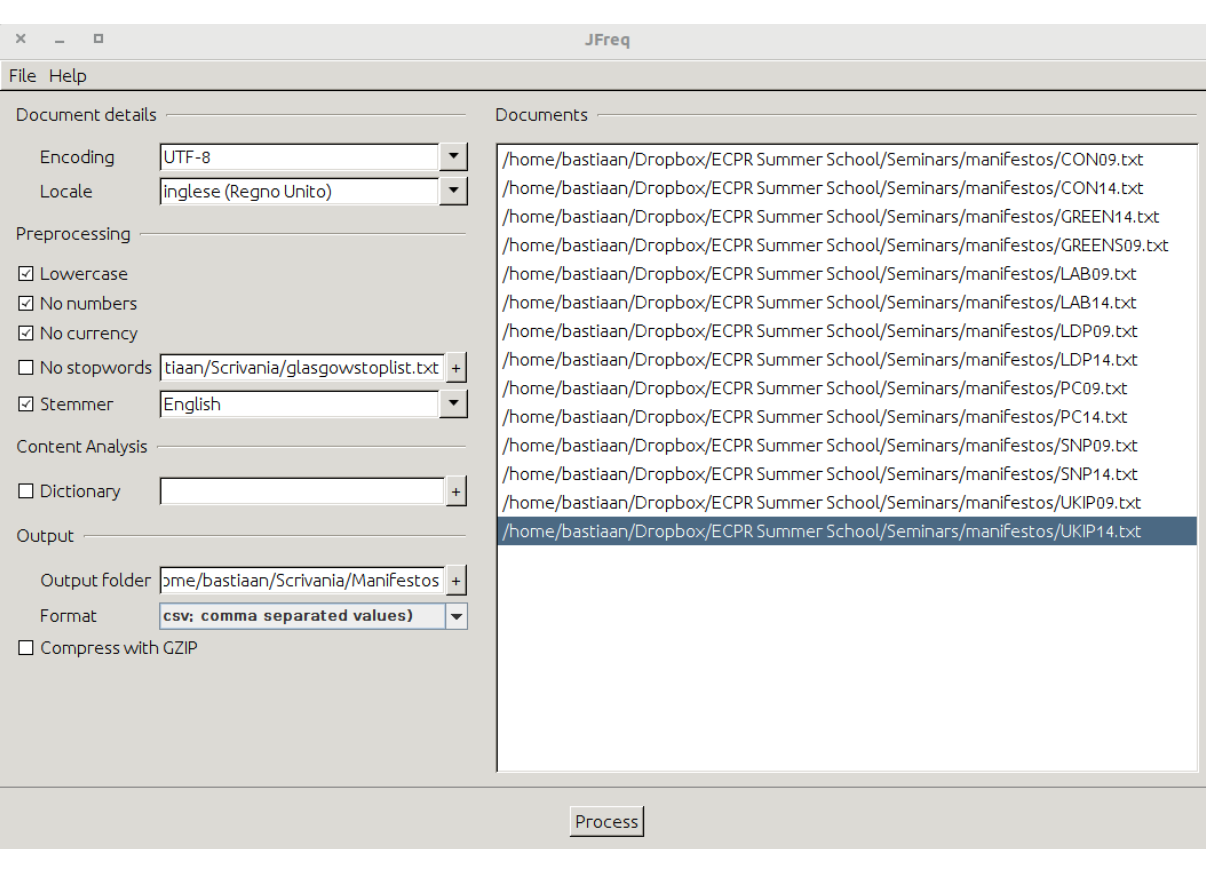
\includegraphics[width=1\linewidth]{figures/jfreq} \caption{Overview of JFreq with several documents loaded}(\#fig:figure-jfreq)
\end{figure}

\hfill\break

Note that here the encoding is UTF-8 while the locale is English (UK). Once we have specified all the options we want, we give a name for the output folder and press \textbf{Process}. Now we go to that folder we named and copy-paste the \textbf{data.csv} file into your Working Directory. In R, we then run the following:

\begin{Shaded}
\begin{Highlighting}[]
\NormalTok{data\_manifestos }\OtherTok{\textless{}{-}} \FunctionTok{read.csv}\NormalTok{(}\StringTok{"data.csv"}\NormalTok{, }\AttributeTok{row.names =} \DecValTok{1}\NormalTok{, }\AttributeTok{header =} \ConstantTok{TRUE}\NormalTok{)}
\end{Highlighting}
\end{Shaded}

By specifying \texttt{row.names=1}, we store the information of the first column in the data frame itself. This column contains the names of the documents, and belongs to the object of the data frame and does not appear as a separate column. The same is true for \texttt{header=TRUE} which ensures that the first row gives names to the columns (in this case containing the words).

\section{Import from an API}\label{import-from-an-api}

Another way to import texts is by using an Application Programming Interface (API). While comparable to web scraping, APIs are much more user friendly and communicate better with R. This makes it easier to download a large amount of data at once and import the results into R. There are APIs for many popular websites, such as Wikipedia, Twitter, YouTube, Weather Underground, The New York Times, the European Union and so on. Note, however, that you often, if not always, need to register before you can use an API. Moreover, social media platforms such as Facebook and Twitter have recently introduced restrictions in the use of their APIs that have limited researchers' ability to conduct critical scholarly research (\citeproc{ref-Bruns2019a}{Bruns, 2019}). For instance, Facebook has taken steps in restricting access to their public APIs for research purposes. As such, free research on Facebook users' posts is no longer an option (\citeproc{ref-Freelon2018a}{Freelon, 2018}; \citeproc{ref-Perriam2020a}{Perriam et al., 2020}). Even more recently, Twitter (rebranded as `X' in July 2023) has \href{https://edition.cnn.com/2023/02/03/tech/twitter-api-what-is-pricing-change-cec/index.html}{eliminated the free access} to its API for third-party developers. At the time of writing, the `Basic' subscription that costs \$100 per month allows you to create a project to pull up to 10,000 Tweets.

While web scraping, in general, is easy with the \texttt{rvest} package, for the APIs you often need a specific package. For example, for Twitter there is the \texttt{rtweet} package, for Facebook \texttt{Rfacebook}, and \texttt{ggmap} for Google maps. Moreover, there are many APIs with associated R packages made by researchers for researchers, such as \texttt{manifestoR}, a package that provides researchers access to the corpus of the Manifesto Project (Merz et al. (\citeproc{ref-Merz2016a}{2016})).

Let's look at an example using an API for the \emph{New York Times}. If you look at the \emph{New York Times}'s API page (\url{https://developer.nytimes.com/}), you will find that we use the API to extract information ranging from opinion articles to book reviews, movie reviews, and so on. In our example, we will use the API to extract a corpus of movie reviews that were originally published in the \emph{New York Times}.

Before we start here, we first have to gain permission to use the API. For this, you need to register an account at the website and log in. Then, make a new \textbf{app} under: \textbf{\url{https://developer.nytimes.com/my-apps}} and ensure you select the movie reviews. Then, you can click on the new app to see your key under \textbf{API Keys}. It is this string of codes and letters you will have to place at the \texttt{{[}YOUR\_API\_KEY\_HERE{]}} bit shown below.

Now, let us first load the necessary packages:

\begin{Shaded}
\begin{Highlighting}[]
\FunctionTok{library}\NormalTok{(tidyverse)}
\FunctionTok{library}\NormalTok{(httr)}
\FunctionTok{library}\NormalTok{(jsonlite)}
\end{Highlighting}
\end{Shaded}

We can then build our request. As you can see on the site, the request requires us to give a search term (here we choose ``love''). Also, we can set a time frame from which we want to extract the reviews:

\begin{Shaded}
\begin{Highlighting}[]
\NormalTok{reviews }\OtherTok{\textless{}{-}} \FunctionTok{fromJSON}\NormalTok{(}\StringTok{"https://api.nytimes.com/svc/movies/v2/reviews/search.json?query=love\&opening{-}date=2000{-}01{-}01:2020{-}01{-}01\&api{-}key=[YOUR\_API\_KEY\_HERE]"}\NormalTok{)}
\end{Highlighting}
\end{Shaded}

The result is a JSON object that you can see in the environment. While JSON (JavaScript Object Notation) is a generic way in which information is easy to share, and is thus often used, it is not in an ideal form. So, we change the JSON information to a data frame using the following:

\begin{Shaded}
\begin{Highlighting}[]
\NormalTok{reviews\_df }\OtherTok{\textless{}{-}} \FunctionTok{fromJSON}\NormalTok{(}\StringTok{"https://api.nytimes.com/svc/movies/v2/reviews/search.json?query=love\&opening{-}date=2000{-}01{-}01:2020{-}01{-}01\&api{-}key=[YOUR\_API\_KEY\_HERE]"}\NormalTok{,}
    \AttributeTok{flatten =} \ConstantTok{TRUE}\NormalTok{) }\SpecialCharTok{\%\textgreater{}\%}
    \FunctionTok{data.frame}\NormalTok{()}
\end{Highlighting}
\end{Shaded}

You can now find all the information in the new \texttt{reviews\_df} object, which also contains other useful information about each movie. As we can see, having a package makes things easier, though more limited.

\section{Import using Web Scraping}\label{import-using-web-scraping}

If there is no specific API, we can also choose to scrape the website. The logic of web scraping is that we use the structure of the underlying HTML document to find and download the text we want. Note though that not all websites encourage (or even allow) scraping, which means that we need to have a look at their disclaimer beforehand. You can do this by either checking the website's \textbf{Terms and Conditions} page, or the \textbf{robots.txt} file that you can usually find appended at the home page (e.g.~\url{https://www.facebook.com/robots.txt} ).

One easy way to scrape a website is to search and see whether someone else has already built a tool that automates the webscraping process for the particular website that we are interested in. For instance, since Twitter has ended the free access to its API, we can look at places like \href{https://apify.com/store?ref=blog.apify.com}{Apify} to find a suitable scraper for popular websites such as Twitter/X, Wikipedia, Instagram (to scrape data on public profiles), Google search, Google maps, Tiktok, Amazon (to scrape data on its products), and so on. Apify is not free, but registering an account for a free trial and using a month's subscription may be enough for a small project.

If you cannot find a ready-made scraper for your project, or if you cannot pay for such services, you can use \texttt{rvest} package to configure a webscraper of your own. One of the most popular sites to scrape is Wikipedia as it is very welcoming to web scraping and has pages with a clear structure (indeed, underlying sites such as WikiData are built with web scraping in mind). Here, let us take the following page on the Cold War as an example: \url{https://en.wikipedia.org/wiki/Cold_War}. If you have a quick look at the website you see that there is a lot of information on there, including figures, tables and the actual body of text. Here, we are only interested in the latter.

To begin with, we store the address of the webpage in an object and ask R to read it for us:

\begin{Shaded}
\begin{Highlighting}[]
\NormalTok{url }\OtherTok{\textless{}{-}} \StringTok{"https://en.wikipedia.org/wiki/Cold\_War"}
\NormalTok{url }\OtherTok{\textless{}{-}}\NormalTok{ rvest}\SpecialCharTok{::}\FunctionTok{read\_html}\NormalTok{(url)}
\end{Highlighting}
\end{Shaded}

We now have the HTML page (though R will not yet show it), but we before we can do anything further, we have to figure out how to get the content we want. To do so, we have to inspect the HTML document to find the right element. The easiest way to do this is in the browser. To do so, open the page and use \textbf{Cmd + Shift + C} to open up Developer Tools. In the tools that then open, we can hover over the main body of text on the page and see which element belongs to it. Here, we find that the main body of text is stored in an element called \textbf{mw-content-text} and that within that the individual paragraphs are stored in elements labelled **

**. This latter designation is a standard reference in HTML to individual paragraphs and are what we are after here.

We now ask R to take the HTML extracted from the URL, look only for the nodes labelled **

**, extract the text from it, place the results into a data frame, and then into a character vector:

\begin{Shaded}
\begin{Highlighting}[]
\FunctionTok{library}\NormalTok{(rvest)}
\end{Highlighting}
\end{Shaded}

\begin{verbatim}
## 
## Attaching package: 'rvest'
\end{verbatim}

\begin{verbatim}
## The following object is masked from 'package:readr':
## 
##     guess_encoding
\end{verbatim}

\begin{Shaded}
\begin{Highlighting}[]
\NormalTok{data\_coldwar }\OtherTok{\textless{}{-}}\NormalTok{ url }\SpecialCharTok{\%\textgreater{}\%}
    \FunctionTok{html\_nodes}\NormalTok{(}\StringTok{"p"}\NormalTok{) }\SpecialCharTok{\%\textgreater{}\%}
    \FunctionTok{html\_text2}\NormalTok{() }\SpecialCharTok{\%\textgreater{}\%}
    \FunctionTok{as.data.frame}\NormalTok{()}
\NormalTok{data\_coldwar }\OtherTok{\textless{}{-}}\NormalTok{ data\_coldwar}\SpecialCharTok{$}\NormalTok{.}
\NormalTok{data\_coldwar }\OtherTok{\textless{}{-}}\NormalTok{ data\_coldwar[}\SpecialCharTok{{-}}\FunctionTok{c}\NormalTok{(}\DecValTok{1}\NormalTok{, }\DecValTok{2}\NormalTok{)]}
\end{Highlighting}
\end{Shaded}

Note that for the text we can choose to use either \texttt{html\_text} or \texttt{html\_text2}. The difference between the two is that while the former gives us the raw underlying text, the latter gives us the text as it looks like in the browser, which is what we opt for here. Now, looking at the resulting data-frame, we have 207 observations representing the 207 paragraphs of the text (with the first two empty, so we removed them here). We can then use this as an input for any further analysis (and we will get back to this later). If you would like to learn more about web scraping in the context of quantitative text analysis have a look at the textbook by Munzert et al. (\citeproc{ref-Munzert2014a}{2014}).

\chapter{Reliability and Validity}\label{reliability-validity}

As noted earlier, as there is no reality we are measuring, there is no way for us to ensure that what we are doing is correct. In other words - everything we do is probably wrong in one way or the other - but it might be useful. So how do we ensure that? To begin with, we should ensure that everything we are do should is both \emph{reliable} and \emph{valid}. Reliability here refers to consistency, that is, the degree to which we get similar results whenever we apply a measuring instrument to measure a given concept. This is similar to the concept of \emph{Replicability}. Validity, on the other hand, refers to unbiasedness, that is, the degree to which our measure does really measure the concept that we intend to measure. In other words, validity looks at whether the measuring instrument that we are using is objective.

Carmines \& Zeller (\citeproc{ref-Carmines1979a}{1979}) distinguish among three types of validity. \emph{Content Validity}, which refers to whether our measure represents all facets of the construct of interest; \emph{Criterion Validity}, which looks at whether our measure correlates with other measures of the same concept, and \emph{Construct Validity}, which looks at whether our measure behaves as expected within a given theoretical context. We should also say here, that these three types of validity are not interchangeable. In the ideal case, one has to prove that their results pass all three validity tests. In the words of Grimmer \& Stewart (\citeproc{ref-Grimmer2013a}{2013}): ``Validate, validate, validate''!

Krippendorff (\citeproc{ref-Krippendorff2004a}{2018}) distinguishes among three types of reliability. The first is \emph{Stability}, which he considers as the weakest form of coding reliability. This we can measure by having our text coded more than once by the same coder. The higher the differences between the different codings, the lower our reliability. The second is \emph{Reproducibility}, which reflects the agreement among independent coders on the same text. Finally, the third is \emph{Accuracy}, which he considers as the strongest form of coding reliability. For this, we look at the agreement between coders, as with reproducibility, but now use a given standard. Yet, as benchmarks are rare, reproducibility is often the highest form we can go for. This agreement between coders we need for this is also known as inter-coder agreement, which we will look at next.

\section{Inter-Coder Agreement}\label{inter-coder-agreement}

Hayes \& Krippendorff (\citeproc{ref-Hayes2007a}{2007, p. 79}) argue that a good measure of the agreement should at least address five criteria. The first is that it should apply to many coders, and not only two. Also, when we use the method for more coders, there should be no difference in how many coders we include. The second is that the method should only take into account the actual number of categories the coders used and not all that were available. This as while the designers designed the coding scheme on what they thought the data would look like, the coders use the scheme based on what the data is. Third, it should be numerical, meaning that we can use it to make a scale between 0 (absence of agreement) and 1 (perfect agreement). Fourth, it should be appropriate for the level of measurement. So, if our data is ordinal or nominal, we should not use a measure that assumes metric data. This ensures that the metric uses all the data and that it does not add or not use other information. Fifth, we should be able to compute (or know), the sampling behaviour of the measure.

With these criteria in mind, we see that popular methods, such as \% agreement or Pearson's \emph{r}, can be misleading. Especially for the latter - as it is a quite popular method - this often leads to problems, as Krippendorff (\citeproc{ref-Krippendorff2004a}{2018}) shows:

\hfill\break

\begin{figure}
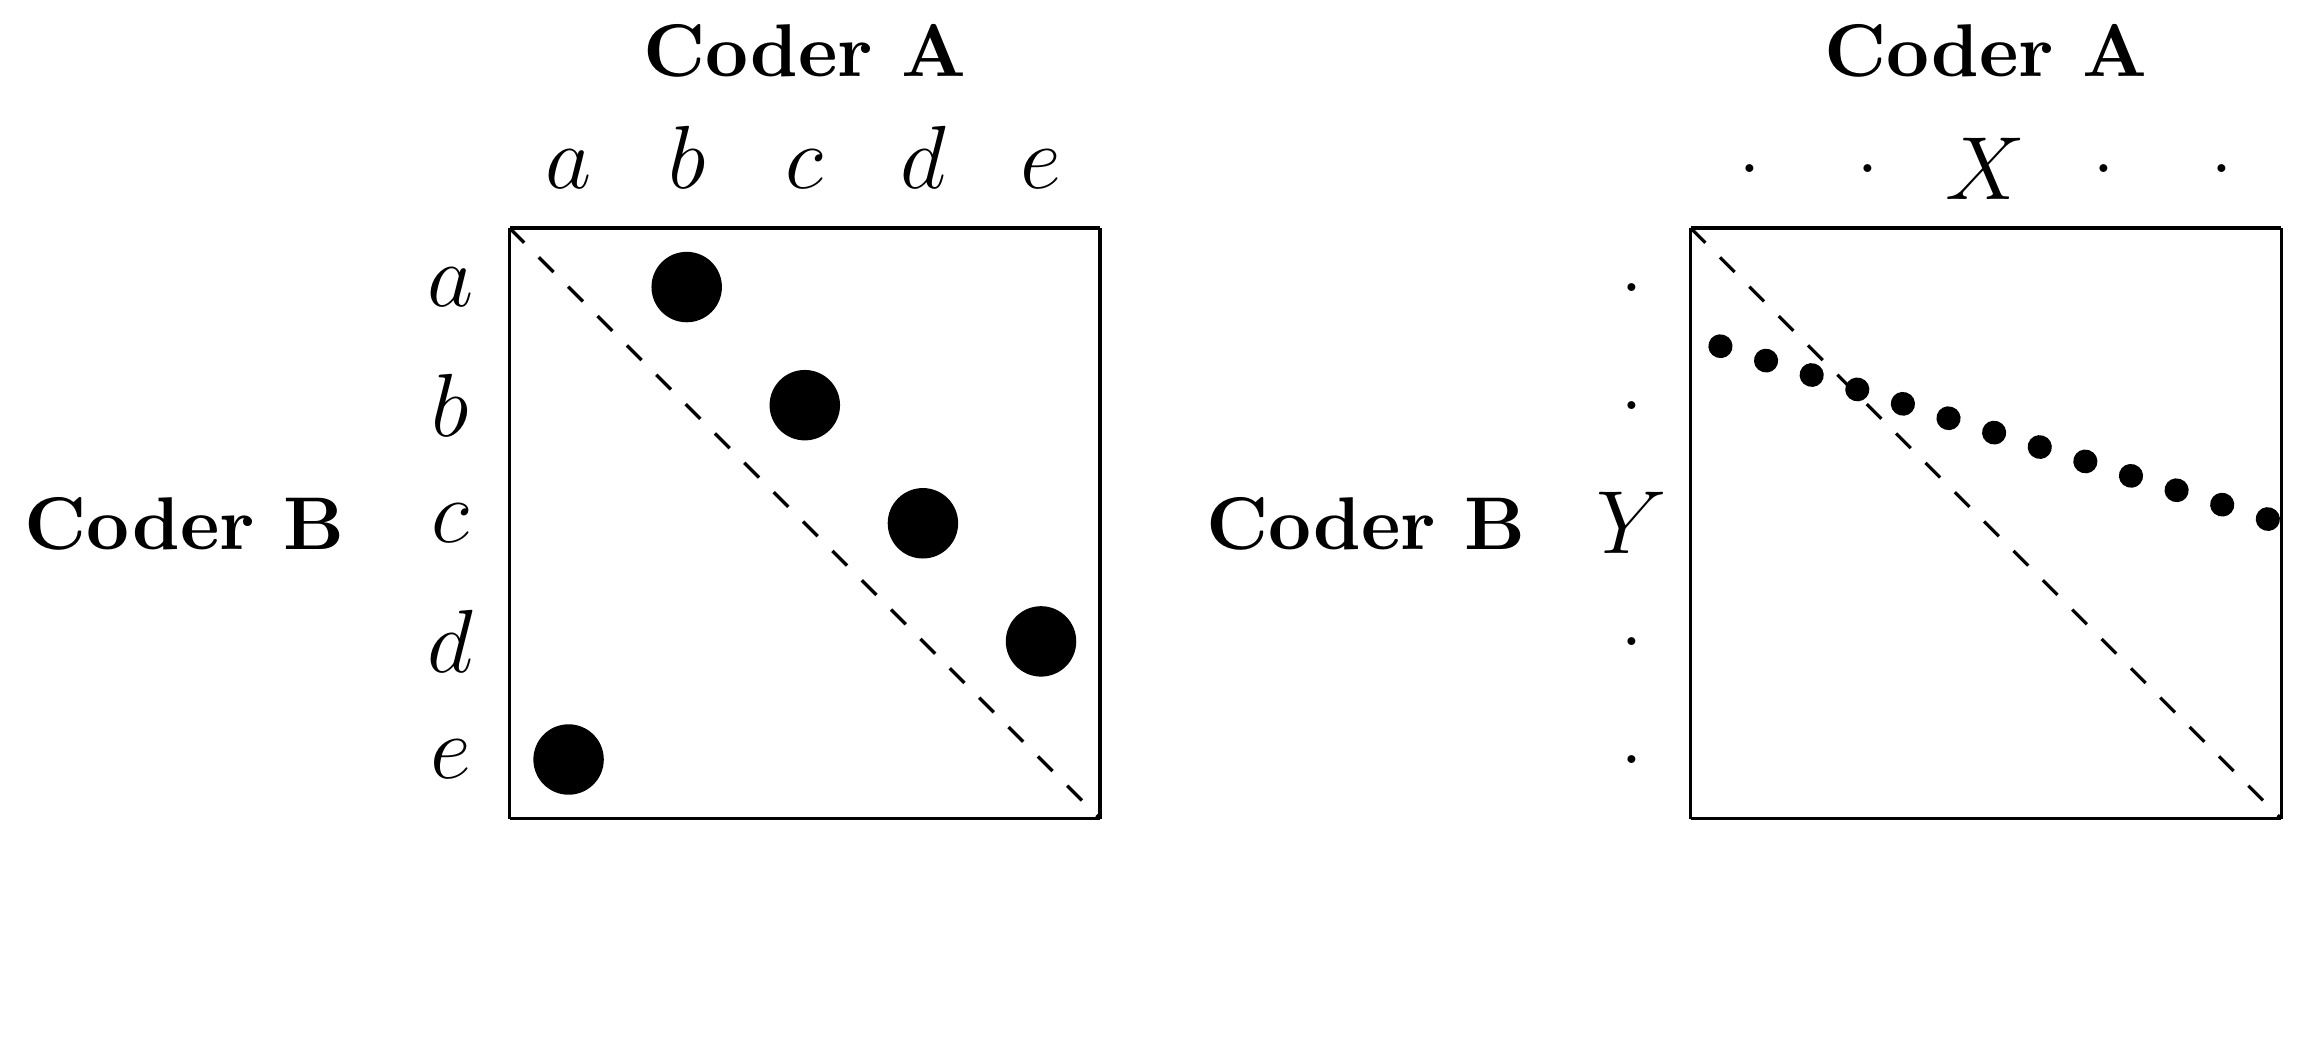
\includegraphics[width=1\linewidth]{_main_files/figure-latex/figure-observers-tikz-1} \caption{Perfect Disagreement between Two Coders [@Krippendorff2004a]}(\#fig:figure-observers-tikz)
\end{figure}

\hfill\break

Here, Figure @ref(fig:figure-observers-tikz) shows, on the left, two coders: A and B. The dots in the figure show the choices both coders made, while the dotted line shows the line of perfect agreement. If a dot is on this line, it means that both Coder A and Coder B made the same choice. In this case, they disagreed in all cases. When Coder A chose \emph{a}, Coder B chose \emph{e}, when Coder A chose \emph{b}, Coder B chose \emph{a}, and so on. Yet, when we would calculate Pearson's \emph{r} for this, we would find a result as shown on the right-hand side of the figure. Seen this way, the agreement between both coders does not seem a problem at all. The reason for this is that Pearson's \emph{r} works with the distances between the categories \emph{without} taking into account their location. So, for a positive relationship, the only thing Pearson's \emph{r} requires is that for every increase or decrease for one coder, there is a similar increase or decrease for the other. This happens here with four of the five categories. The result is thus a high Pearson's \emph{r}, though the actual agreement should be 0.

Pearson's \emph{r} thus cannot fulfil all our criteria. A measure that can is Krippendorff's \(\alpha\) (\citeproc{ref-Krippendorff2004a}{Krippendorff, 2018}). This measure can not only give us the agreement we need, but can also do so for nominal, ordinal, interval, and ratio level data, as well as data with many coders and missing values. Besides, we can compute 95\% confidence intervals around \(\alpha\) using bootstrapping, which we can use to show the degree of uncertainty around our reliability estimates.

Despite this, Krippendorff's \(\alpha\) is not free of problems. One main problem occurs when coders agree on only a few categories and use these categories a considerable number of times. This leads to an inflation of \(\alpha\), making it is higher than it should be (\citeproc{ref-Krippendorff2004a}{Krippendorff, 2018}), as in the following example:

\hfill\break

\begin{figure}
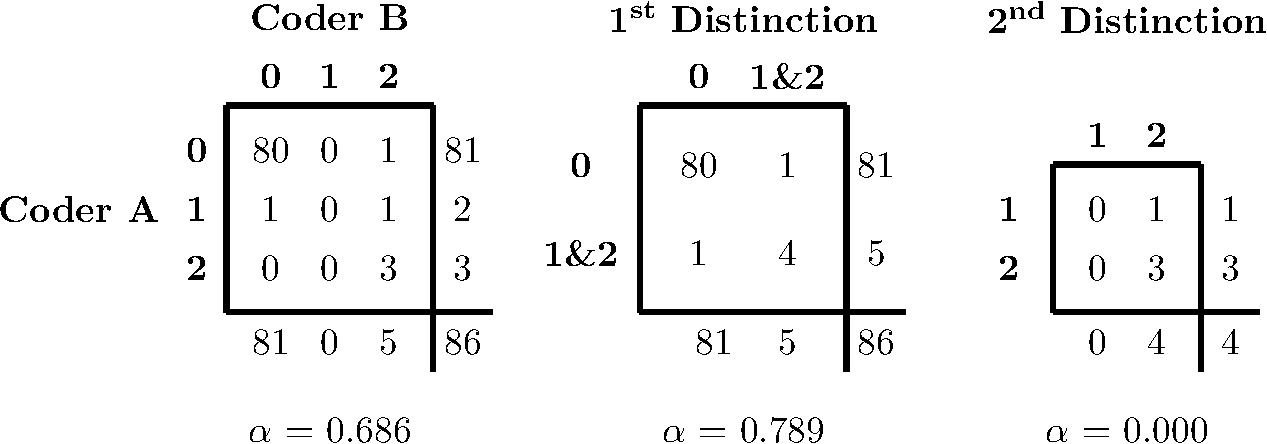
\includegraphics[width=1\linewidth]{_main_files/figure-latex/figure-kripp-tikz-1} \caption{Possible Inflation of Krippendorff's` $\alpha$ [@Krippendorff2004a]}(\#fig:figure-kripp-tikz)
\end{figure}

\hfill\break

Here, the top left of the figure shows coders A and B, who have to code into three categories: 0, 1, or 2. In this example, categories 1 and 2 carry a certain meaning, while category 0 means that the coders did not know what to assign the case to. Of the 86 cases, both coders code 80 cases in the 0 category. This means that there are only 6 cases on which they can agree or disagree about a code that carries some meaning. Yet, if we calculate \(\alpha\), the result - 0.686 - takes into account all the categories. One solution for this is to add up categories 1 and 2, as the figure in the middle shows. Here, the coders agree in 84 of the 86 cases (on the diagonal line) and disagree in only 2 of them. Calculating \(\alpha\) now shows that it would increase to 0.789. Finally, we can remove the 0 category and again view 1 and 2 as separate categories (as the most right-hand figure shows). Yet, the result of this is quite disastrous. While the coders agree in 3 of the 4 cases, the resulting \(\alpha\) equals 0.000, as coder B did not use category 1 at all.

Apart from these issues, Krippendorff's \(\alpha\) is a stable and useful measure. A value of \(\alpha\) = 1 indicates perfect reliability, while a value of \(\alpha\) = 0 indicates the absence of reliability. This means that if \(\alpha\) = 0, there is no relationship between the values. It is possible for \(\alpha\) \textless{} 0, which means that the disagreements between the values are larger than they would be by chance and are systematic. As for thresholds, Krippendorff (\citeproc{ref-Krippendorff2004a}{2018}) proposes to use either 0.80 or 0.67 for results to be reliable. Such low reliability often has many causes. One thing might be that the coding scheme is not appropriate for the documents. This means that coders had categories that they had no use for, and lacked categories they needed. Another reason might be that the coders lacked training. Thus, they did not understand how to use the coding scheme or how the coding process works. This often leads to frustration on part of the coders, as in these cases the process often becomes time-consuming and too demanding to carry out.

To calculate Krippendorff's \(\alpha\), we can use the following software:

\begin{itemize}
\tightlist
\item
  KALPHA custom dialogue (SPSS)
\item
  \textbf{kalpha} user-written package (Stata)
\item
  KALPHA macro (SAS)
\item
  \texttt{kripp.alpha} command in \texttt{kripp.boot} package (R) - amongst others
\end{itemize}

Let us try this in R using an example. Here, we will look at the results of a coding reliability test where 12 coders assigned the sentences of the 1997 European Commission work programme in the 20 categories of a policy areas coding scheme. We can find the results for this on GitHub. To get the data, we tell R where to find it, then to read that file as a .csv file and write it to a new object:

\begin{Shaded}
\begin{Highlighting}[]
\FunctionTok{library}\NormalTok{(readr)}

\NormalTok{urlfile }\OtherTok{=} \StringTok{"https://raw.githubusercontent.com/SCJBruinsma/qta{-}files/master/reliability\_results.csv"}
\NormalTok{reliability\_results }\OtherTok{\textless{}{-}} \FunctionTok{read\_csv}\NormalTok{(}\FunctionTok{url}\NormalTok{(urlfile), }\AttributeTok{show\_col\_types =} \ConstantTok{FALSE}\NormalTok{)}
\end{Highlighting}
\end{Shaded}

Notice that in the data frame we created, the coders are in the columns and the sentences in the rows. As the \texttt{kripp.boot} package requires it to be the other way around and in matrix form, we first transpose the data and then place it in a matrix. Finally, we run the command and specify we want the nominal version:

\begin{Shaded}
\begin{Highlighting}[]
\FunctionTok{library}\NormalTok{(}\StringTok{"kripp.boot"}\NormalTok{)}

\NormalTok{reliability\_results\_t }\OtherTok{\textless{}{-}} \FunctionTok{t}\NormalTok{(reliability\_results)}
\NormalTok{reliability }\OtherTok{\textless{}{-}} \FunctionTok{as.matrix}\NormalTok{(reliability\_results\_t)}
\NormalTok{kalpha }\OtherTok{\textless{}{-}} \FunctionTok{kripp.boot}\NormalTok{(reliability, }\AttributeTok{iter =} \DecValTok{1000}\NormalTok{, }\AttributeTok{method =} \StringTok{"nominal"}\NormalTok{)}
\NormalTok{kalpha}\SpecialCharTok{$}\NormalTok{mean.alpha}
\end{Highlighting}
\end{Shaded}

Note also that \texttt{kripp.boot} is a GitHub package. You can still calculate the value (but without the confidence interval) with another package:

\begin{Shaded}
\begin{Highlighting}[]
\FunctionTok{library}\NormalTok{(}\StringTok{"DescTools"}\NormalTok{)}

\NormalTok{reliability\_results\_t }\OtherTok{\textless{}{-}} \FunctionTok{t}\NormalTok{(reliability\_results)}
\NormalTok{reliability }\OtherTok{\textless{}{-}} \FunctionTok{as.matrix}\NormalTok{(reliability\_results\_t)}
\NormalTok{kalpha }\OtherTok{\textless{}{-}} \FunctionTok{KrippAlpha}\NormalTok{(reliability, }\AttributeTok{method =} \StringTok{"nominal"}\NormalTok{)}
\NormalTok{kalpha}\SpecialCharTok{$}\NormalTok{value}
\end{Highlighting}
\end{Shaded}

As we can see, the results point out that the agreement among the coders is 0.634 with an upper limit of 0.650 and a lower limit of 0.618 which is short of Krippendorff's cut-off point of 0.667.

\section{Visualizing Quality}\label{visualizing-quality}

Lamprianou (\citeproc{ref-Lamprianou2020a}{2020}) notes that existing reliability indices may mask coding problems and that the reliability of coding is not stable across coding units (as illustrated in the example given for Krippendorff's \(\alpha\) above). To investigate the quality of coding he proposes using social network analysis (SNA) and exponential random graph models (ERGM). Here, we illustrate a different approach, based on the idea of sensitivity analysis.

The idea of this is to compare the codings of each coder against all others (and also against a benchmark or a gold standard). To do so, we need to bootstrap the coding reliability results to create an uncertainty measure around each coder's results, following the approach proposed by Benoit et al. (\citeproc{ref-Benoit2009a}{2009}). The idea here is to use a non-parametric bootstrap for the codings of each coder (using 1000 draws with replacement) at the category level and then calculate the confidence intervals. Their width then depends on both the number of sentences coded by each coder (n) in each category and the number of coding categories that are not empty. Thus, larger documents and fewer empty categories result in narrower confidence intervals, while a small number of categories leads to wider intervals (\citeproc{ref-Lowe2011a}{Lowe \& Benoit, 2011}).

To start, the first thing we do is load the packages we need into R:

\begin{Shaded}
\begin{Highlighting}[]
\FunctionTok{library}\NormalTok{(Hmisc)}
\end{Highlighting}
\end{Shaded}

\begin{verbatim}
## Warning: package 'Hmisc' was built under R version 4.3.3
\end{verbatim}

\begin{Shaded}
\begin{Highlighting}[]
\FunctionTok{library}\NormalTok{(combinat)}
\FunctionTok{library}\NormalTok{(readr)}
\end{Highlighting}
\end{Shaded}

In the following example we perform the sensitivity analysis on the coded sentences of the 1997 European Commission work programme, as seen earlier. Yet here, row represents a coder, and each column represents a coding category (\texttt{c0} to \texttt{c19}). In each cell, we see the number of sentences that each coder coded in each category, with the column \texttt{n} giving the sum of each row:

\begin{Shaded}
\begin{Highlighting}[]
\NormalTok{urlfile }\OtherTok{\textless{}{-}} \StringTok{"https://raw.githubusercontent.com/SCJBruinsma/qta{-}book/main/data\_uncertainty.csv"}
\NormalTok{data\_uncertainty }\OtherTok{\textless{}{-}} \FunctionTok{read\_csv}\NormalTok{(}\FunctionTok{url}\NormalTok{(urlfile))}
\end{Highlighting}
\end{Shaded}

We then tell R how many coders we have. As this number is equal to the number of rows we have, we can get this number using the \texttt{nrow} command. We also specify the number of bootstraps we want to carry out (1000) and transform our data frame into an array. We do the latter as R needs the data in this format later on:

\begin{Shaded}
\begin{Highlighting}[]
\NormalTok{nman }\OtherTok{\textless{}{-}} \FunctionTok{nrow}\NormalTok{(data\_uncertainty)}
\NormalTok{nrepl }\OtherTok{\textless{}{-}} \DecValTok{1000}
\NormalTok{manifBSn }\OtherTok{\textless{}{-}}
\NormalTok{  manifBSnRand }\OtherTok{\textless{}{-}} \FunctionTok{array}\NormalTok{(}
    \FunctionTok{as.matrix}\NormalTok{(data\_uncertainty[, }\DecValTok{2}\SpecialCharTok{:}\DecValTok{21}\NormalTok{]),}
    \FunctionTok{c}\NormalTok{(nman, }\DecValTok{20}\NormalTok{, nrepl }\SpecialCharTok{+} \DecValTok{1}\NormalTok{),}
    \AttributeTok{dimnames =} \FunctionTok{list}\NormalTok{(}\DecValTok{1}\SpecialCharTok{:}\NormalTok{nman, }\FunctionTok{names}\NormalTok{(data\_uncertainty[, }\DecValTok{2}\SpecialCharTok{:}\DecValTok{21}\NormalTok{]),}
                    \DecValTok{0}\SpecialCharTok{:}\NormalTok{nrepl)}
\NormalTok{  )}
\end{Highlighting}
\end{Shaded}

We then bootstrap the sentence counts for each coder and compute percentages for each category using a multinomial draw. First, we define \texttt{p}, which is the proportion of each category over all the coders. Then, we input this value together with the total number of codes \texttt{n} into the \texttt{rmultinomial} command, which gives the random draws. As we want to do this a 1000 times, we place this command into a \texttt{for} loop:

\begin{Shaded}
\begin{Highlighting}[]
\NormalTok{n }\OtherTok{\textless{}{-}}\NormalTok{ data\_uncertainty}\SpecialCharTok{$}\NormalTok{n}
\NormalTok{p }\OtherTok{\textless{}{-}}\NormalTok{ manifBSn[, , }\DecValTok{1}\NormalTok{] }\SpecialCharTok{/}\NormalTok{ n}

\ControlFlowTok{for}\NormalTok{ (i }\ControlFlowTok{in} \DecValTok{1}\SpecialCharTok{:}\NormalTok{nrepl) \{}
\NormalTok{  manifBSn[, , i] }\OtherTok{\textless{}{-}} \FunctionTok{rmultinomial}\NormalTok{(n, p)}
\NormalTok{\}}
\end{Highlighting}
\end{Shaded}

With this data, we can then ask R to compute the quantities of interest. These are standard errors for each category, as well as the percentage coded for each category:

\begin{Shaded}
\begin{Highlighting}[]
\NormalTok{c0SE  }\OtherTok{\textless{}{-}} \FunctionTok{apply}\NormalTok{(manifBSn[, }\StringTok{"c0"}\NormalTok{, ]  }\SpecialCharTok{/}\NormalTok{ n }\SpecialCharTok{*} \DecValTok{100}\NormalTok{, }\DecValTok{1}\NormalTok{, sd)}
\NormalTok{c01SE }\OtherTok{\textless{}{-}} \FunctionTok{apply}\NormalTok{(manifBSn[, }\StringTok{"c01"}\NormalTok{, ] }\SpecialCharTok{/}\NormalTok{ n }\SpecialCharTok{*} \DecValTok{100}\NormalTok{, }\DecValTok{1}\NormalTok{, sd)}
\NormalTok{c02SE }\OtherTok{\textless{}{-}} \FunctionTok{apply}\NormalTok{(manifBSn[, }\StringTok{"c02"}\NormalTok{, ] }\SpecialCharTok{/}\NormalTok{ n }\SpecialCharTok{*} \DecValTok{100}\NormalTok{, }\DecValTok{1}\NormalTok{, sd)}
\NormalTok{c03SE }\OtherTok{\textless{}{-}} \FunctionTok{apply}\NormalTok{(manifBSn[, }\StringTok{"c03"}\NormalTok{, ] }\SpecialCharTok{/}\NormalTok{ n }\SpecialCharTok{*} \DecValTok{100}\NormalTok{, }\DecValTok{1}\NormalTok{, sd)}
\NormalTok{c04SE }\OtherTok{\textless{}{-}} \FunctionTok{apply}\NormalTok{(manifBSn[, }\StringTok{"c04"}\NormalTok{, ] }\SpecialCharTok{/}\NormalTok{ n }\SpecialCharTok{*} \DecValTok{100}\NormalTok{, }\DecValTok{1}\NormalTok{, sd)}
\NormalTok{c05SE }\OtherTok{\textless{}{-}} \FunctionTok{apply}\NormalTok{(manifBSn[, }\StringTok{"c05"}\NormalTok{, ] }\SpecialCharTok{/}\NormalTok{ n }\SpecialCharTok{*} \DecValTok{100}\NormalTok{, }\DecValTok{1}\NormalTok{, sd)}
\NormalTok{c06SE }\OtherTok{\textless{}{-}} \FunctionTok{apply}\NormalTok{(manifBSn[, }\StringTok{"c06"}\NormalTok{, ] }\SpecialCharTok{/}\NormalTok{ n }\SpecialCharTok{*} \DecValTok{100}\NormalTok{, }\DecValTok{1}\NormalTok{, sd)}
\NormalTok{c07SE }\OtherTok{\textless{}{-}} \FunctionTok{apply}\NormalTok{(manifBSn[, }\StringTok{"c07"}\NormalTok{, ] }\SpecialCharTok{/}\NormalTok{ n }\SpecialCharTok{*} \DecValTok{100}\NormalTok{, }\DecValTok{1}\NormalTok{, sd)}
\NormalTok{c08SE }\OtherTok{\textless{}{-}} \FunctionTok{apply}\NormalTok{(manifBSn[, }\StringTok{"c08"}\NormalTok{, ] }\SpecialCharTok{/}\NormalTok{ n }\SpecialCharTok{*} \DecValTok{100}\NormalTok{, }\DecValTok{1}\NormalTok{, sd)}
\NormalTok{c09SE }\OtherTok{\textless{}{-}} \FunctionTok{apply}\NormalTok{(manifBSn[, }\StringTok{"c09"}\NormalTok{, ] }\SpecialCharTok{/}\NormalTok{ n }\SpecialCharTok{*} \DecValTok{100}\NormalTok{, }\DecValTok{1}\NormalTok{, sd)}
\NormalTok{c10SE }\OtherTok{\textless{}{-}} \FunctionTok{apply}\NormalTok{(manifBSn[, }\StringTok{"c10"}\NormalTok{, ] }\SpecialCharTok{/}\NormalTok{ n }\SpecialCharTok{*} \DecValTok{100}\NormalTok{, }\DecValTok{1}\NormalTok{, sd)}
\NormalTok{c11SE }\OtherTok{\textless{}{-}} \FunctionTok{apply}\NormalTok{(manifBSn[, }\StringTok{"c11"}\NormalTok{, ] }\SpecialCharTok{/}\NormalTok{ n }\SpecialCharTok{*} \DecValTok{100}\NormalTok{, }\DecValTok{1}\NormalTok{, sd)}
\NormalTok{c12SE }\OtherTok{\textless{}{-}} \FunctionTok{apply}\NormalTok{(manifBSn[, }\StringTok{"c12"}\NormalTok{, ] }\SpecialCharTok{/}\NormalTok{ n }\SpecialCharTok{*} \DecValTok{100}\NormalTok{, }\DecValTok{1}\NormalTok{, sd)}
\NormalTok{c13SE }\OtherTok{\textless{}{-}} \FunctionTok{apply}\NormalTok{(manifBSn[, }\StringTok{"c13"}\NormalTok{, ] }\SpecialCharTok{/}\NormalTok{ n }\SpecialCharTok{*} \DecValTok{100}\NormalTok{, }\DecValTok{1}\NormalTok{, sd)}
\NormalTok{c14SE }\OtherTok{\textless{}{-}} \FunctionTok{apply}\NormalTok{(manifBSn[, }\StringTok{"c14"}\NormalTok{, ] }\SpecialCharTok{/}\NormalTok{ n }\SpecialCharTok{*} \DecValTok{100}\NormalTok{, }\DecValTok{1}\NormalTok{, sd)}
\NormalTok{c15SE }\OtherTok{\textless{}{-}} \FunctionTok{apply}\NormalTok{(manifBSn[, }\StringTok{"c15"}\NormalTok{, ] }\SpecialCharTok{/}\NormalTok{ n }\SpecialCharTok{*} \DecValTok{100}\NormalTok{, }\DecValTok{1}\NormalTok{, sd)}
\NormalTok{c16SE }\OtherTok{\textless{}{-}} \FunctionTok{apply}\NormalTok{(manifBSn[, }\StringTok{"c16"}\NormalTok{, ] }\SpecialCharTok{/}\NormalTok{ n }\SpecialCharTok{*} \DecValTok{100}\NormalTok{, }\DecValTok{1}\NormalTok{, sd)}
\NormalTok{c17SE }\OtherTok{\textless{}{-}} \FunctionTok{apply}\NormalTok{(manifBSn[, }\StringTok{"c17"}\NormalTok{, ] }\SpecialCharTok{/}\NormalTok{ n }\SpecialCharTok{*} \DecValTok{100}\NormalTok{, }\DecValTok{1}\NormalTok{, sd)}
\NormalTok{c18SE }\OtherTok{\textless{}{-}} \FunctionTok{apply}\NormalTok{(manifBSn[, }\StringTok{"c18"}\NormalTok{, ] }\SpecialCharTok{/}\NormalTok{ n }\SpecialCharTok{*} \DecValTok{100}\NormalTok{, }\DecValTok{1}\NormalTok{, sd)}
\NormalTok{c19SE }\OtherTok{\textless{}{-}} \FunctionTok{apply}\NormalTok{(manifBSn[, }\StringTok{"c19"}\NormalTok{, ] }\SpecialCharTok{/}\NormalTok{ n }\SpecialCharTok{*} \DecValTok{100}\NormalTok{, }\DecValTok{1}\NormalTok{, sd)}

\NormalTok{per0  }\OtherTok{\textless{}{-}} \FunctionTok{apply}\NormalTok{(manifBSn[, }\StringTok{"c0"}\NormalTok{, ]  }\SpecialCharTok{/}\NormalTok{ n }\SpecialCharTok{*} \DecValTok{100}\NormalTok{, }\DecValTok{1}\NormalTok{, mean)}
\NormalTok{per01 }\OtherTok{\textless{}{-}} \FunctionTok{apply}\NormalTok{(manifBSn[, }\StringTok{"c01"}\NormalTok{, ] }\SpecialCharTok{/}\NormalTok{ n }\SpecialCharTok{*} \DecValTok{100}\NormalTok{, }\DecValTok{1}\NormalTok{, mean)}
\NormalTok{per02 }\OtherTok{\textless{}{-}} \FunctionTok{apply}\NormalTok{(manifBSn[, }\StringTok{"c02"}\NormalTok{, ] }\SpecialCharTok{/}\NormalTok{ n }\SpecialCharTok{*} \DecValTok{100}\NormalTok{, }\DecValTok{1}\NormalTok{, mean)}
\NormalTok{per03 }\OtherTok{\textless{}{-}} \FunctionTok{apply}\NormalTok{(manifBSn[, }\StringTok{"c03"}\NormalTok{, ] }\SpecialCharTok{/}\NormalTok{ n }\SpecialCharTok{*} \DecValTok{100}\NormalTok{, }\DecValTok{1}\NormalTok{, mean)}
\NormalTok{per04 }\OtherTok{\textless{}{-}} \FunctionTok{apply}\NormalTok{(manifBSn[, }\StringTok{"c04"}\NormalTok{, ] }\SpecialCharTok{/}\NormalTok{ n }\SpecialCharTok{*} \DecValTok{100}\NormalTok{, }\DecValTok{1}\NormalTok{, mean)}
\NormalTok{per05 }\OtherTok{\textless{}{-}} \FunctionTok{apply}\NormalTok{(manifBSn[, }\StringTok{"c05"}\NormalTok{, ] }\SpecialCharTok{/}\NormalTok{ n }\SpecialCharTok{*} \DecValTok{100}\NormalTok{, }\DecValTok{1}\NormalTok{, mean)}
\NormalTok{per06 }\OtherTok{\textless{}{-}} \FunctionTok{apply}\NormalTok{(manifBSn[, }\StringTok{"c06"}\NormalTok{, ] }\SpecialCharTok{/}\NormalTok{ n }\SpecialCharTok{*} \DecValTok{100}\NormalTok{, }\DecValTok{1}\NormalTok{, mean)}
\NormalTok{per07 }\OtherTok{\textless{}{-}} \FunctionTok{apply}\NormalTok{(manifBSn[, }\StringTok{"c07"}\NormalTok{, ] }\SpecialCharTok{/}\NormalTok{ n }\SpecialCharTok{*} \DecValTok{100}\NormalTok{, }\DecValTok{1}\NormalTok{, mean)}
\NormalTok{per08 }\OtherTok{\textless{}{-}} \FunctionTok{apply}\NormalTok{(manifBSn[, }\StringTok{"c08"}\NormalTok{, ] }\SpecialCharTok{/}\NormalTok{ n }\SpecialCharTok{*} \DecValTok{100}\NormalTok{, }\DecValTok{1}\NormalTok{, mean)}
\NormalTok{per09 }\OtherTok{\textless{}{-}} \FunctionTok{apply}\NormalTok{(manifBSn[, }\StringTok{"c09"}\NormalTok{, ] }\SpecialCharTok{/}\NormalTok{ n }\SpecialCharTok{*} \DecValTok{100}\NormalTok{, }\DecValTok{1}\NormalTok{, mean)}
\NormalTok{per10 }\OtherTok{\textless{}{-}} \FunctionTok{apply}\NormalTok{(manifBSn[, }\StringTok{"c10"}\NormalTok{, ] }\SpecialCharTok{/}\NormalTok{ n }\SpecialCharTok{*} \DecValTok{100}\NormalTok{, }\DecValTok{1}\NormalTok{, mean)}
\NormalTok{per11 }\OtherTok{\textless{}{-}} \FunctionTok{apply}\NormalTok{(manifBSn[, }\StringTok{"c11"}\NormalTok{, ] }\SpecialCharTok{/}\NormalTok{ n }\SpecialCharTok{*} \DecValTok{100}\NormalTok{, }\DecValTok{1}\NormalTok{, mean)}
\NormalTok{per12 }\OtherTok{\textless{}{-}} \FunctionTok{apply}\NormalTok{(manifBSn[, }\StringTok{"c12"}\NormalTok{, ] }\SpecialCharTok{/}\NormalTok{ n }\SpecialCharTok{*} \DecValTok{100}\NormalTok{, }\DecValTok{1}\NormalTok{, mean)}
\NormalTok{per13 }\OtherTok{\textless{}{-}} \FunctionTok{apply}\NormalTok{(manifBSn[, }\StringTok{"c13"}\NormalTok{, ] }\SpecialCharTok{/}\NormalTok{ n }\SpecialCharTok{*} \DecValTok{100}\NormalTok{, }\DecValTok{1}\NormalTok{, mean)}
\NormalTok{per14 }\OtherTok{\textless{}{-}} \FunctionTok{apply}\NormalTok{(manifBSn[, }\StringTok{"c14"}\NormalTok{, ] }\SpecialCharTok{/}\NormalTok{ n }\SpecialCharTok{*} \DecValTok{100}\NormalTok{, }\DecValTok{1}\NormalTok{, mean)}
\NormalTok{per15 }\OtherTok{\textless{}{-}} \FunctionTok{apply}\NormalTok{(manifBSn[, }\StringTok{"c15"}\NormalTok{, ] }\SpecialCharTok{/}\NormalTok{ n }\SpecialCharTok{*} \DecValTok{100}\NormalTok{, }\DecValTok{1}\NormalTok{, mean)}
\NormalTok{per16 }\OtherTok{\textless{}{-}} \FunctionTok{apply}\NormalTok{(manifBSn[, }\StringTok{"c16"}\NormalTok{, ] }\SpecialCharTok{/}\NormalTok{ n }\SpecialCharTok{*} \DecValTok{100}\NormalTok{, }\DecValTok{1}\NormalTok{, mean)}
\NormalTok{per17 }\OtherTok{\textless{}{-}} \FunctionTok{apply}\NormalTok{(manifBSn[, }\StringTok{"c17"}\NormalTok{, ] }\SpecialCharTok{/}\NormalTok{ n }\SpecialCharTok{*} \DecValTok{100}\NormalTok{, }\DecValTok{1}\NormalTok{, mean)}
\NormalTok{per18 }\OtherTok{\textless{}{-}} \FunctionTok{apply}\NormalTok{(manifBSn[, }\StringTok{"c18"}\NormalTok{, ] }\SpecialCharTok{/}\NormalTok{ n }\SpecialCharTok{*} \DecValTok{100}\NormalTok{, }\DecValTok{1}\NormalTok{, mean)}
\NormalTok{per19 }\OtherTok{\textless{}{-}} \FunctionTok{apply}\NormalTok{(manifBSn[, }\StringTok{"c19"}\NormalTok{, ] }\SpecialCharTok{/}\NormalTok{ n }\SpecialCharTok{*} \DecValTok{100}\NormalTok{, }\DecValTok{1}\NormalTok{, mean)}
\end{Highlighting}
\end{Shaded}

We then bind all these quantities together in a single data frame:

\begin{Shaded}
\begin{Highlighting}[]
\NormalTok{dataBS }\OtherTok{\textless{}{-}} \FunctionTok{data.frame}\NormalTok{(}\FunctionTok{cbind}\NormalTok{(data\_uncertainty[, }\DecValTok{1}\SpecialCharTok{:}\DecValTok{22}\NormalTok{], c0SE, c01SE, c02SE, c03SE, c04SE,}
\NormalTok{    c05SE, c06SE, c07SE, c08SE, c09SE, c10SE, c11SE, c12SE, c13SE, c14SE, c15SE,}
\NormalTok{    c16SE, c17SE, c18SE, c19SE, per0, per01, per02, per03, per04, per05, per06, per07,}
\NormalTok{    per08, per09, per10, per11, per12, per13, per14, per15, per16, per17, per18,}
\NormalTok{    per19))}
\end{Highlighting}
\end{Shaded}

While we can now inspect the results by looking at the data, it becomes more clear when we visualise this. While R has some inbuilt tools for visualisation (in the \texttt{graphics} package), these tools are rather crude. Thus, here we will use the \texttt{ggplot2} package, which extends our options, and which has an intuitive structure:

\begin{Shaded}
\begin{Highlighting}[]
\FunctionTok{library}\NormalTok{(ggplot2)}
\end{Highlighting}
\end{Shaded}

First, we make sure that the variable \texttt{coderid} is a factor and make sure that it is in the right order:

\begin{Shaded}
\begin{Highlighting}[]
\NormalTok{dataBS}\SpecialCharTok{$}\NormalTok{coderid }\OtherTok{\textless{}{-}} \FunctionTok{as.factor}\NormalTok{(dataBS}\SpecialCharTok{$}\NormalTok{coderid)}
\NormalTok{dataBS}\SpecialCharTok{$}\NormalTok{coderid }\OtherTok{\textless{}{-}} \FunctionTok{factor}\NormalTok{(dataBS}\SpecialCharTok{$}\NormalTok{coderid, }\FunctionTok{levels}\NormalTok{(dataBS}\SpecialCharTok{$}\NormalTok{coderid)[}\FunctionTok{c}\NormalTok{(}\DecValTok{1}\NormalTok{, }\DecValTok{5}\SpecialCharTok{:}\DecValTok{12}\NormalTok{, }\DecValTok{2}\SpecialCharTok{:}\DecValTok{4}\NormalTok{)])}
\end{Highlighting}
\end{Shaded}

Then, we calculate the 95\% confidence intervals for each category. We do so using the percent of each category and the respective standard error, and add these values to our data-set:

\begin{Shaded}
\begin{Highlighting}[]
\NormalTok{c0\_lo }\OtherTok{\textless{}{-}}\NormalTok{ per0 }\SpecialCharTok{{-}}\NormalTok{ (}\FloatTok{1.96} \SpecialCharTok{*}\NormalTok{ c0SE)}
\NormalTok{c0\_hi }\OtherTok{\textless{}{-}}\NormalTok{ per0 }\SpecialCharTok{+}\NormalTok{ (}\FloatTok{1.96} \SpecialCharTok{*}\NormalTok{ c0SE)}
\NormalTok{c01\_lo }\OtherTok{\textless{}{-}}\NormalTok{ per01 }\SpecialCharTok{{-}}\NormalTok{ (}\FloatTok{1.96} \SpecialCharTok{*}\NormalTok{ c01SE)}
\NormalTok{c01\_hi }\OtherTok{\textless{}{-}}\NormalTok{ per01 }\SpecialCharTok{+}\NormalTok{ (}\FloatTok{1.96} \SpecialCharTok{*}\NormalTok{ c01SE)}
\NormalTok{c02\_lo }\OtherTok{\textless{}{-}}\NormalTok{ per02 }\SpecialCharTok{{-}}\NormalTok{ (}\FloatTok{1.96} \SpecialCharTok{*}\NormalTok{ c02SE)}
\NormalTok{c02\_hi }\OtherTok{\textless{}{-}}\NormalTok{ per02 }\SpecialCharTok{+}\NormalTok{ (}\FloatTok{1.96} \SpecialCharTok{*}\NormalTok{ c02SE)}

\NormalTok{dataBS }\OtherTok{\textless{}{-}} \FunctionTok{cbind}\NormalTok{(dataBS, c0\_lo, c0\_hi, c01\_lo, c01\_hi, c02\_lo, c02\_hi)}
\end{Highlighting}
\end{Shaded}

Finally, we generate the graphs for each individual category:

\begin{Shaded}
\begin{Highlighting}[]
\FunctionTok{ggplot}\NormalTok{(dataBS,}\FunctionTok{aes}\NormalTok{(per0, coderid))}\SpecialCharTok{+}
 \FunctionTok{geom\_point}\NormalTok{() }\SpecialCharTok{+}
 \FunctionTok{geom\_errorbarh}\NormalTok{(}\FunctionTok{aes}\NormalTok{(}\AttributeTok{xmax =}\NormalTok{ c0\_hi, }\AttributeTok{xmin =}\NormalTok{ c0\_lo),}\AttributeTok{height =}\NormalTok{ .}\DecValTok{2}\NormalTok{)}\SpecialCharTok{+}
 \FunctionTok{xlab}\NormalTok{(}\StringTok{"Percentage coded to category 0"}\NormalTok{)}\SpecialCharTok{+}
 \FunctionTok{ylab}\NormalTok{(}\StringTok{"Coder ID"}\NormalTok{)}\SpecialCharTok{+}
 \FunctionTok{theme\_classic}\NormalTok{()}
\end{Highlighting}
\end{Shaded}

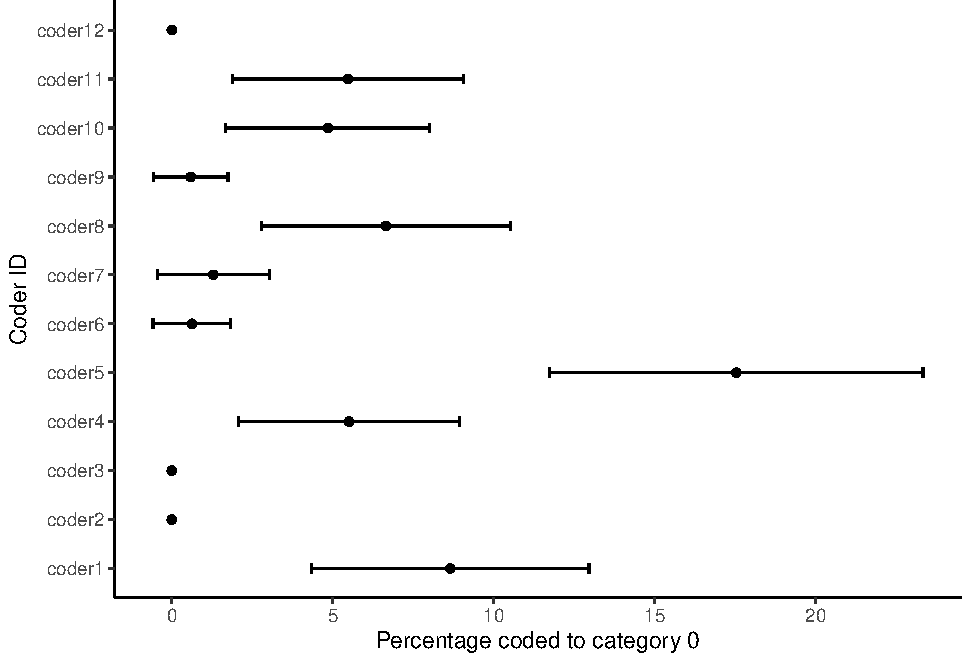
\includegraphics{_main_files/figure-latex/coder-category0-1.pdf}

\begin{Shaded}
\begin{Highlighting}[]
\FunctionTok{ggplot}\NormalTok{(dataBS,}\FunctionTok{aes}\NormalTok{(per01, coderid))}\SpecialCharTok{+}
 \FunctionTok{geom\_point}\NormalTok{() }\SpecialCharTok{+}
 \FunctionTok{geom\_errorbarh}\NormalTok{(}\FunctionTok{aes}\NormalTok{(}\AttributeTok{xmax =}\NormalTok{ c01\_hi, }\AttributeTok{xmin =}\NormalTok{ c01\_lo),}\AttributeTok{height =}\NormalTok{ .}\DecValTok{2}\NormalTok{)}\SpecialCharTok{+}
 \FunctionTok{xlab}\NormalTok{(}\StringTok{"Percentage coded to category 01"}\NormalTok{)}\SpecialCharTok{+}
 \FunctionTok{ylab}\NormalTok{(}\StringTok{"Coder ID"}\NormalTok{)}\SpecialCharTok{+}
 \FunctionTok{theme\_classic}\NormalTok{()}
\end{Highlighting}
\end{Shaded}

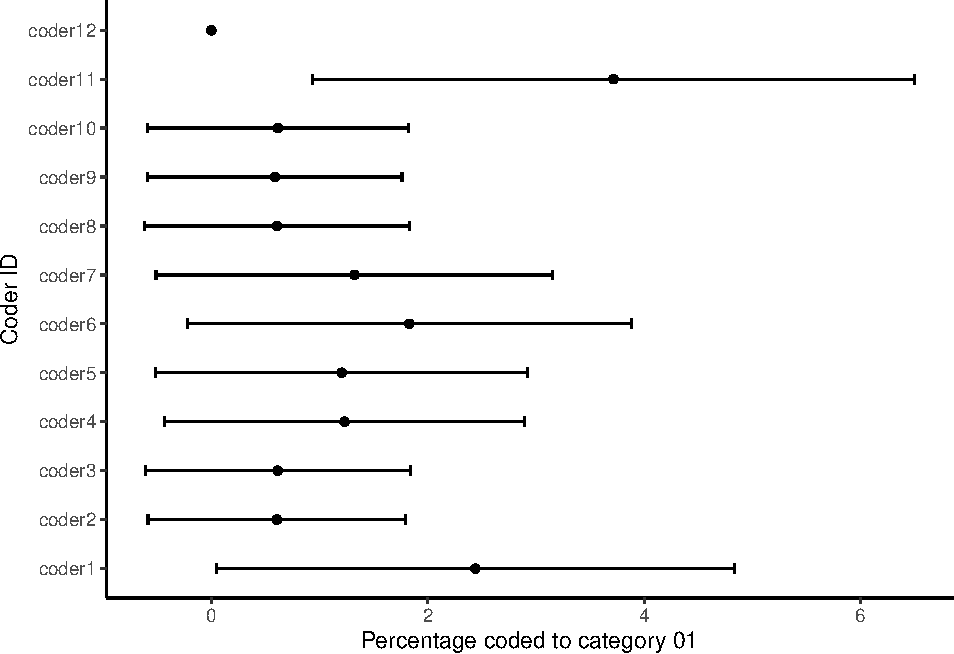
\includegraphics{_main_files/figure-latex/coder-category1-1.pdf}

\begin{Shaded}
\begin{Highlighting}[]
\FunctionTok{ggplot}\NormalTok{(dataBS,}\FunctionTok{aes}\NormalTok{(per02, coderid))}\SpecialCharTok{+}
 \FunctionTok{geom\_point}\NormalTok{() }\SpecialCharTok{+}
 \FunctionTok{geom\_errorbarh}\NormalTok{(}\FunctionTok{aes}\NormalTok{(}\AttributeTok{xmax =}\NormalTok{ c02\_hi, }\AttributeTok{xmin =}\NormalTok{ c02\_lo),}\AttributeTok{height =}\NormalTok{ .}\DecValTok{2}\NormalTok{)}\SpecialCharTok{+}
 \FunctionTok{xlab}\NormalTok{(}\StringTok{"Percentage coded to category 02"}\NormalTok{)}\SpecialCharTok{+}
 \FunctionTok{ylab}\NormalTok{(}\StringTok{"Coder ID"}\NormalTok{)}\SpecialCharTok{+}
 \FunctionTok{theme\_classic}\NormalTok{()}
\end{Highlighting}
\end{Shaded}

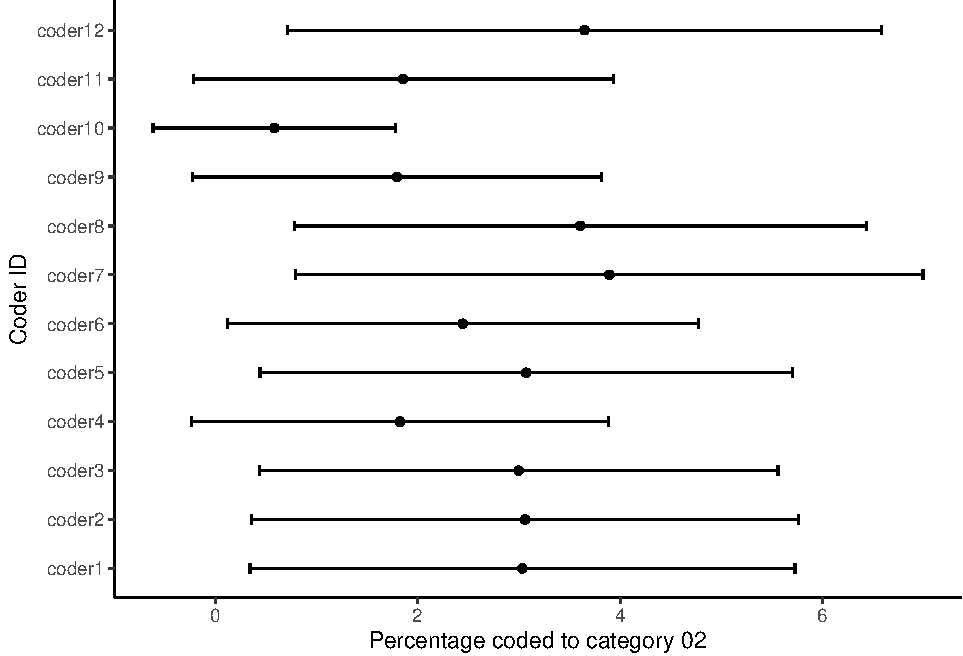
\includegraphics{_main_files/figure-latex/coder-category2-1.pdf}

Each figure shows the percentage that each of the coders coded in the respective category of the coding scheme. We thus use the confidence intervals around the estimates to look at the degree of uncertainty around each estimate. We can read the plots by looking if the dashed line is within the confidence intervals for each coder. The more the coders deviate from the benchmark or standard, the less likely it is that they understood the coding scheme in the same way. It also means that it is more likely that a coder would have coded the work programme much different from the benchmark coder. Thus, such a sensitivity analysis is like having a single reliability coefficient for each coding category.

\chapter{Preliminaries}\label{preliminaries}

Now that we have loaded our texts into R, it is time to understand \emph{what} our texts are about, who their authors are, and what we can expect to find in them. Here we will look at three different techniques for doing this: keywords-in-context, visualisations and text statistics. Before that, however, we will have a brief look at the idea of the \emph{corpus}, as it is central to the idea of how \texttt{quanteda} works.

\section{The Corpus}\label{the-corpus}

Within \texttt{quanteda}, the main way to store documents is in the form of a \texttt{corpus} object. This object contains all the information that comes with the texts and does not change during our analysis. Instead, we make copies of the main corpus, convert them to the type we need and run our analyses on them. The advantage of this is that we can always go back to our original data.

There are various ways to make a corpus. One we already saw in the @ref(importing-data) chapter were we used \texttt{readtext} to generate a data frame, with both a variable that gave us a \textbf{doc\_id} and another that gave us the text. As \texttt{readtext} and \texttt{quanteda} work close together, we can directly change this to a corpus. Alternatively, we can take a character vector, where each element of the vector is taken as an individual document. If the vector is named, those names will be used as document names - if not, new ones are generated.

Here, let us go back to the Cold War page we scraped earlier and use the resulting text from that as our input:

\begin{Shaded}
\begin{Highlighting}[]
\NormalTok{url }\OtherTok{\textless{}{-}} \StringTok{"https://en.wikipedia.org/wiki/Cold\_War"}
\NormalTok{url }\OtherTok{\textless{}{-}}\NormalTok{ rvest}\SpecialCharTok{::}\FunctionTok{read\_html}\NormalTok{(url)}
\NormalTok{data\_coldwar }\OtherTok{\textless{}{-}}\NormalTok{ url }\SpecialCharTok{\%\textgreater{}\%}
    \FunctionTok{html\_nodes}\NormalTok{(}\StringTok{"p"}\NormalTok{) }\SpecialCharTok{\%\textgreater{}\%}
    \FunctionTok{html\_text2}\NormalTok{() }\SpecialCharTok{\%\textgreater{}\%}
    \FunctionTok{as.data.frame}\NormalTok{()}
\NormalTok{data\_coldwar }\OtherTok{\textless{}{-}}\NormalTok{ data\_coldwar}\SpecialCharTok{$}\NormalTok{.}
\NormalTok{data\_coldwar }\OtherTok{\textless{}{-}}\NormalTok{ data\_coldwar[}\SpecialCharTok{{-}}\FunctionTok{c}\NormalTok{(}\DecValTok{1}\NormalTok{, }\DecValTok{2}\NormalTok{)]}
\end{Highlighting}
\end{Shaded}

Note that the resulting \texttt{data\_coldwar} vector is unnamed, so \texttt{quanteda} will generate those names for us. Now, we simply put this into the \texttt{corpus} command:

\begin{Shaded}
\begin{Highlighting}[]
\FunctionTok{library}\NormalTok{(quanteda)}
\end{Highlighting}
\end{Shaded}

\begin{verbatim}
## Warning: package 'quanteda' was built under R version 4.3.3
\end{verbatim}

\begin{verbatim}
## Package version: 4.0.2
## Unicode version: 15.1
## ICU version: 74.1
\end{verbatim}

\begin{verbatim}
## Parallel computing: 8 of 8 threads used.
\end{verbatim}

\begin{verbatim}
## See https://quanteda.io for tutorials and examples.
\end{verbatim}

\begin{Shaded}
\begin{Highlighting}[]
\NormalTok{data\_corpus }\OtherTok{\textless{}{-}} \FunctionTok{corpus}\NormalTok{(data\_coldwar)}
\end{Highlighting}
\end{Shaded}

Apart from importing texts ourselves, \texttt{quanteda} contains several corpora as well. Here, we use one of these, which contains the inaugural speeches of all the US Presidents. For this, we first have to load the main package and then load the data into R:

Now we have our corpus, we can start with the analysis. As noted, we try not to carry out any analysis on the corpus itself. Instead, we keep it as it is and work on its copies. Often, this means transforming the data into another shape. One of the more popular shapes is the \emph{data frequency matrix} (dfm). This is a matrix that contains the documents in the rows and the word counts for each word in the columns.

Before we can do so, we have to split up our texts into unique words. To do this, we first have to construct a \texttt{tokens} object. In the command that we use to do this, we can specify how we want to split our texts (here we use the standard option) and how we want to clean our data. For example, we can specify that we want to convert all the texts into lowercase and remove any numbers and special characters.

\begin{Shaded}
\begin{Highlighting}[]
\NormalTok{data\_tokens }\OtherTok{\textless{}{-}} \FunctionTok{tokens}\NormalTok{(}
\NormalTok{ data\_corpus,}
 \AttributeTok{what =} \StringTok{"word"}\NormalTok{,}
 \AttributeTok{remove\_punct =} \ConstantTok{TRUE}\NormalTok{,}
 \AttributeTok{remove\_symbols =} \ConstantTok{TRUE}\NormalTok{,}
 \AttributeTok{remove\_numbers =} \ConstantTok{TRUE}\NormalTok{,}
 \AttributeTok{remove\_url =} \ConstantTok{TRUE}\NormalTok{,}
 \AttributeTok{remove\_separators =} \ConstantTok{TRUE}\NormalTok{,}
 \AttributeTok{split\_hyphens =} \ConstantTok{FALSE}\NormalTok{,}
 \AttributeTok{include\_docvars =} \ConstantTok{TRUE}\NormalTok{,}
 \AttributeTok{padding =} \ConstantTok{FALSE}\NormalTok{,}
 \AttributeTok{verbose =} \ConstantTok{TRUE}
\NormalTok{)}
\end{Highlighting}
\end{Shaded}

We can also remove certain stopwords so that words like ``and'' or ``the'' do not influence our analysis too much. We can either specify these words ourselves or we can use a list that is already present in R. To see this list, type \texttt{stopwords("english")} in the console. Stopwords for other languages are also available (such as German, French and Spanish). There are even more stopwords in the \texttt{stopwords} package, which works well with \texttt{quanteda}. For now, we will use the English ones. As all the stopwords here are lower-case, we will have to lower case our words as well. Also notice that we also do this for any acronyms in our text (so, ``NATO'' will become ``nato''):

\begin{Shaded}
\begin{Highlighting}[]
\NormalTok{data\_tokens }\OtherTok{\textless{}{-}} \FunctionTok{tokens\_tolower}\NormalTok{(data\_tokens,}
                              \AttributeTok{keep\_acronyms =} \ConstantTok{FALSE}\NormalTok{)}
\NormalTok{data\_tokens }\OtherTok{\textless{}{-}} \FunctionTok{tokens\_select}\NormalTok{(data\_tokens,}
                             \FunctionTok{stopwords}\NormalTok{(}\StringTok{"english"}\NormalTok{),}
                             \AttributeTok{selection =} \StringTok{"remove"}\NormalTok{)}
\end{Highlighting}
\end{Shaded}

Then, we can construct our dfm:

\begin{Shaded}
\begin{Highlighting}[]
\NormalTok{data\_dfm }\OtherTok{\textless{}{-}} \FunctionTok{dfm}\NormalTok{(data\_tokens)}
\end{Highlighting}
\end{Shaded}

\section{Keywords in Context}\label{keywords-in-context}

One simple - but effective - way to learn more about our texts is by looking at keywords-in-context (kwic). Here, we look at with which other words a certain word appears in our texts. This is also known as looking at the \emph{concordance} of our text. To do so is easy with our tokens data frame. Let's take all those words that start with `secur' and look at which three words occur before and after this word. We can then run:

\begin{Shaded}
\begin{Highlighting}[]
\NormalTok{kwic\_output }\OtherTok{\textless{}{-}} \FunctionTok{kwic}\NormalTok{(data\_tokens, }\AttributeTok{pattern =} \StringTok{"secur*"}\NormalTok{, }\AttributeTok{valuetype =} \StringTok{"glob"}\NormalTok{, }\AttributeTok{window =} \DecValTok{3}\NormalTok{)}
\end{Highlighting}
\end{Shaded}

In the outputted object, we find a column labelled \texttt{pre} and another labelled \texttt{post}. These refer to the words that came either before or after the word 'secur*'. We can easily take these out and combine them:

\begin{Shaded}
\begin{Highlighting}[]
\NormalTok{text\_pre }\OtherTok{\textless{}{-}}\NormalTok{ kwic\_output}\SpecialCharTok{$}\NormalTok{pre}
\NormalTok{text\_post }\OtherTok{\textless{}{-}}\NormalTok{ kwic\_output}\SpecialCharTok{$}\NormalTok{post}
\NormalTok{text\_word }\OtherTok{\textless{}{-}}\NormalTok{ kwic\_output}\SpecialCharTok{$}\NormalTok{keyword}
\NormalTok{text }\OtherTok{\textless{}{-}} \FunctionTok{as.data.frame}\NormalTok{(}\FunctionTok{paste}\NormalTok{(text\_pre, text\_word, text\_post))}
\end{Highlighting}
\end{Shaded}

We then combine this information with the name of the document it came from so that we know which text the word is from:

\begin{Shaded}
\begin{Highlighting}[]
\NormalTok{extracted }\OtherTok{\textless{}{-}} \FunctionTok{cbind}\NormalTok{(kwic\_output}\SpecialCharTok{$}\NormalTok{docname, text)}
\FunctionTok{names}\NormalTok{(extracted) }\OtherTok{\textless{}{-}} \FunctionTok{c}\NormalTok{(}\StringTok{"docname"}\NormalTok{, }\StringTok{"text"}\NormalTok{)}
\FunctionTok{head}\NormalTok{(extracted)}
\end{Highlighting}
\end{Shaded}

\begin{verbatim}
##   docname                                                                 text
## 1  text10             making allowances peace security ushering period détente
## 2  text27 establishment maintenance post-war security scholars contend western
## 3  text27        western allies desired security system democratic governments
## 4  text27  churchill's mainly centered securing control mediterranean ensuring
## 5  text34    peace enforcement capacity security council effectively paralyzed
## 6  text44        leaders establishing secret security force prevent subversion
\end{verbatim}

\section{Visualisations and Descriptives}\label{visualisations-and-descriptives}

Another thing we can do is generate various visualisations to understand our data. One interesting thing can be to see which words occur most often. We can do this using the \texttt{topfeatures} function. For this, we first have to save the 50 most frequently occurring words in our texts (note that there is also the \texttt{textstat\_frequency} function in the \texttt{quanteda.textstats} helper package that can do this):

\begin{Shaded}
\begin{Highlighting}[]
\NormalTok{features }\OtherTok{\textless{}{-}} \FunctionTok{topfeatures}\NormalTok{(data\_dfm, }\DecValTok{50}\NormalTok{)}
\end{Highlighting}
\end{Shaded}

We then have to transform this object into a data frame, and sort it by decreasing frequency:

\begin{Shaded}
\begin{Highlighting}[]
\NormalTok{features\_plot }\OtherTok{\textless{}{-}} \FunctionTok{data.frame}\NormalTok{(}\FunctionTok{list}\NormalTok{(}\AttributeTok{term =} \FunctionTok{names}\NormalTok{(features),}\AttributeTok{frequency =} \FunctionTok{unname}\NormalTok{(features)))}
\NormalTok{features\_plot}\SpecialCharTok{$}\NormalTok{term }\OtherTok{\textless{}{-}} \FunctionTok{with}\NormalTok{(features\_plot, }\FunctionTok{reorder}\NormalTok{(term, }\SpecialCharTok{{-}}\NormalTok{frequency))}
\end{Highlighting}
\end{Shaded}

Then we can plot the results:

\begin{Shaded}
\begin{Highlighting}[]
\FunctionTok{library}\NormalTok{(ggplot2)}
\FunctionTok{ggplot}\NormalTok{(features\_plot) }\SpecialCharTok{+} 
 \FunctionTok{geom\_point}\NormalTok{(}\FunctionTok{aes}\NormalTok{(}\AttributeTok{x=}\NormalTok{term, }\AttributeTok{y=}\NormalTok{frequency)) }\SpecialCharTok{+}
 \FunctionTok{theme\_classic}\NormalTok{()}\SpecialCharTok{+}
 \FunctionTok{theme}\NormalTok{(}\AttributeTok{axis.text.x=}\FunctionTok{element\_text}\NormalTok{(}\AttributeTok{angle=}\DecValTok{90}\NormalTok{, }\AttributeTok{hjust=}\DecValTok{1}\NormalTok{))}
\end{Highlighting}
\end{Shaded}

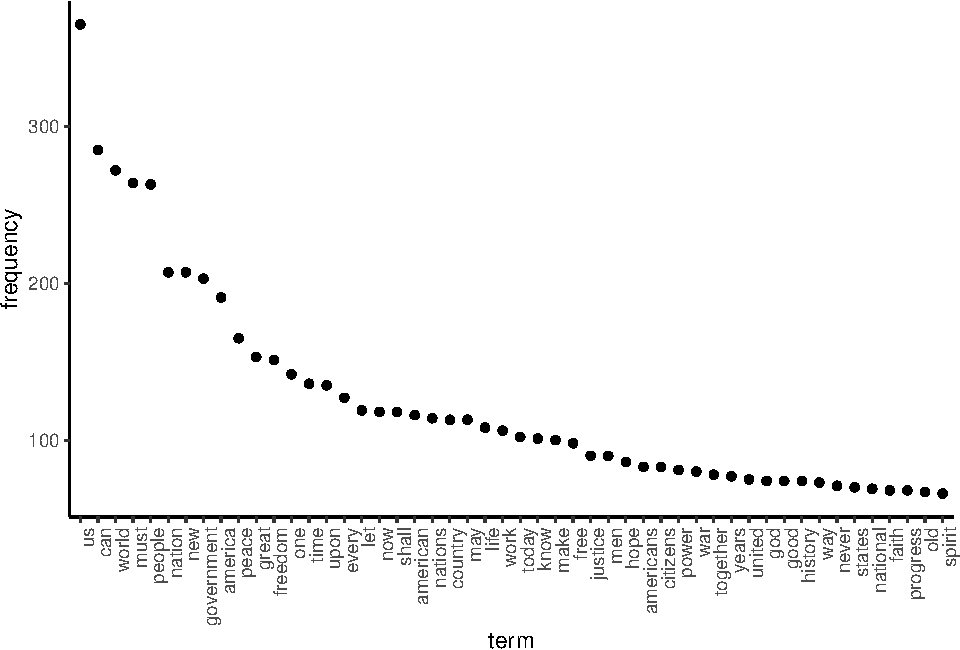
\includegraphics{_main_files/figure-latex/topfeatures-ggplot-1.pdf}

We can also generate word clouds. As these show all the words we have, we will trim our dfm first to remove all those words that occurred less than 30 times. We can do this with the \texttt{dfm\_trim} function. Then, we can use this trimmed dfm to generate the word cloud:

\begin{Shaded}
\begin{Highlighting}[]
\FunctionTok{library}\NormalTok{(quanteda.textplots)}

\NormalTok{wordcloud\_dfm\_trim }\OtherTok{\textless{}{-}} \FunctionTok{dfm\_trim}\NormalTok{(data\_dfm, }\AttributeTok{min\_termfreq =} \DecValTok{10}\NormalTok{)}
\FunctionTok{textplot\_wordcloud}\NormalTok{(wordcloud\_dfm\_trim)}
\end{Highlighting}
\end{Shaded}


\includegraphics{_main_files/figure-latex/wordcloud-inaugural-1.pdf}

\section{Text Statistics}\label{text-statistics}

Finally, \texttt{quanteda} also allows us to calculate quite some textual statistics. These are all collected in the \texttt{quanteda.textstats} helper package. Here, we will look at several of them, starting with a simple overview of our corpus in the terms of a summary. This tells us the number of characters, sentences, tokens, etc. for each of the texts:

\begin{Shaded}
\begin{Highlighting}[]
\FunctionTok{library}\NormalTok{(quanteda.textstats)}
\end{Highlighting}
\end{Shaded}

\begin{verbatim}
## Warning: package 'quanteda.textstats' was built under R version 4.3.3
\end{verbatim}

\begin{Shaded}
\begin{Highlighting}[]
\NormalTok{corpus\_summary }\OtherTok{\textless{}{-}} \FunctionTok{textstat\_summary}\NormalTok{(data\_corpus)}
\end{Highlighting}
\end{Shaded}

If we want, we can then use this data to make some simple graphs telling us various things about the texts in our corpus. As an example, let's look at the number of sentences in the various paragraphs:

\begin{Shaded}
\begin{Highlighting}[]
\FunctionTok{ggplot}\NormalTok{(}\AttributeTok{data=}\NormalTok{corpus\_summary, }\FunctionTok{aes}\NormalTok{(}\AttributeTok{x=}\NormalTok{document, }\AttributeTok{y=}\NormalTok{sents, }\AttributeTok{group=}\DecValTok{1}\NormalTok{)) }\SpecialCharTok{+}
 \FunctionTok{geom\_line}\NormalTok{()}\SpecialCharTok{+}
 \FunctionTok{geom\_point}\NormalTok{()}\SpecialCharTok{+}
 \FunctionTok{ylab}\NormalTok{(}\StringTok{"Number of Characters"}\NormalTok{)}\SpecialCharTok{+}
 \FunctionTok{xlab}\NormalTok{(}\StringTok{"Paragraph"}\NormalTok{)}\SpecialCharTok{+}
 \FunctionTok{theme\_classic}\NormalTok{()}\SpecialCharTok{+}
 \FunctionTok{theme}\NormalTok{(}\AttributeTok{axis.text.x =} \FunctionTok{element\_text}\NormalTok{(}\AttributeTok{angle =} \DecValTok{90}\NormalTok{))}
\end{Highlighting}
\end{Shaded}

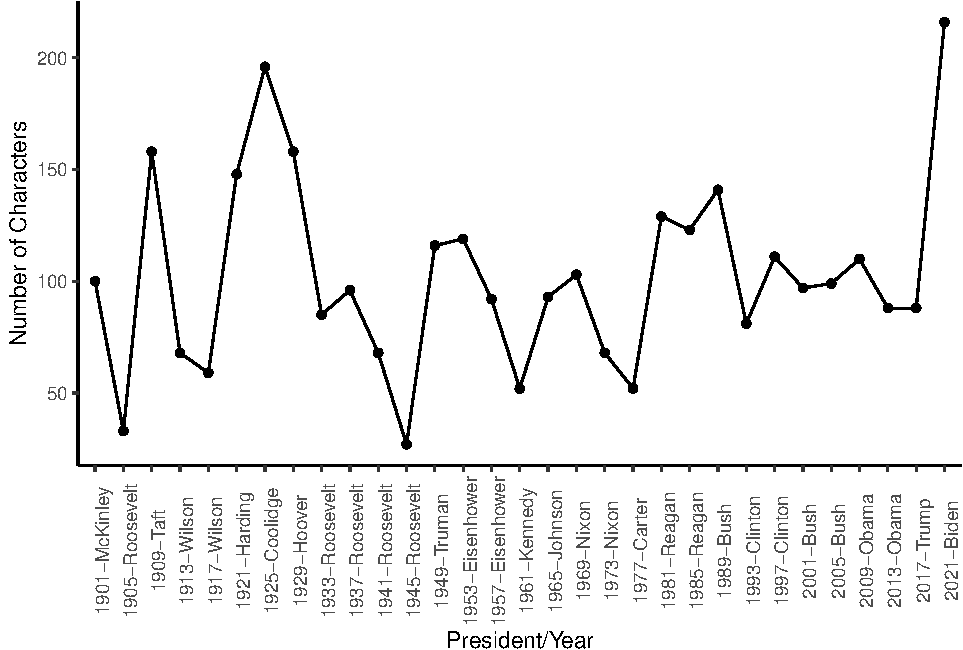
\includegraphics{_main_files/figure-latex/ggplot-summary-1.pdf}

Other things we can look at are the readability and lexical diversity of the texts. The former one of these refers to how readable a text is (i.e.~how easy or difficult it is to read), while the latter tells us how many different types of words there are in the texts and thus how \emph{diverse} the text is in word choice and use. Given that there are many ways to calculate both metrics, please have a look at the help file to see which one works best for you. Here, we will use the most popular:

\begin{Shaded}
\begin{Highlighting}[]
\NormalTok{corpus\_readability }\OtherTok{\textless{}{-}} \FunctionTok{textstat\_readability}\NormalTok{(data\_corpus, }\AttributeTok{measure =} \StringTok{"Flesch.Kincaid"}\NormalTok{)}
\NormalTok{corpus\_lexdiv }\OtherTok{\textless{}{-}} \FunctionTok{textstat\_lexdiv}\NormalTok{(data\_tokens, }\AttributeTok{measure =} \StringTok{"CTTR"}\NormalTok{)}
\end{Highlighting}
\end{Shaded}

As before, we can plot this data in a graph to see how lexical diversity developed over the course of the article:

\begin{Shaded}
\begin{Highlighting}[]
\FunctionTok{ggplot}\NormalTok{(}\AttributeTok{data=}\NormalTok{corpus\_lexdiv, }\FunctionTok{aes}\NormalTok{(}\AttributeTok{x=}\NormalTok{document, }\AttributeTok{y=}\NormalTok{CTTR, }\AttributeTok{group=}\DecValTok{1}\NormalTok{)) }\SpecialCharTok{+}
 \FunctionTok{geom\_line}\NormalTok{()}\SpecialCharTok{+}
 \FunctionTok{geom\_point}\NormalTok{()}\SpecialCharTok{+}
 \FunctionTok{ylab}\NormalTok{(}\StringTok{"Lexical Diversity (CTTR)"}\NormalTok{)}\SpecialCharTok{+}
 \FunctionTok{xlab}\NormalTok{(}\StringTok{"Paragraph"}\NormalTok{)}\SpecialCharTok{+}
 \FunctionTok{theme\_classic}\NormalTok{()}\SpecialCharTok{+}
 \FunctionTok{theme}\NormalTok{(}\AttributeTok{axis.text.x =} \FunctionTok{element\_text}\NormalTok{(}\AttributeTok{angle =} \DecValTok{90}\NormalTok{))}
\end{Highlighting}
\end{Shaded}

\begin{verbatim}
## Warning: Removed 1 row containing missing values or values outside the scale range
## (`geom_point()`).
\end{verbatim}

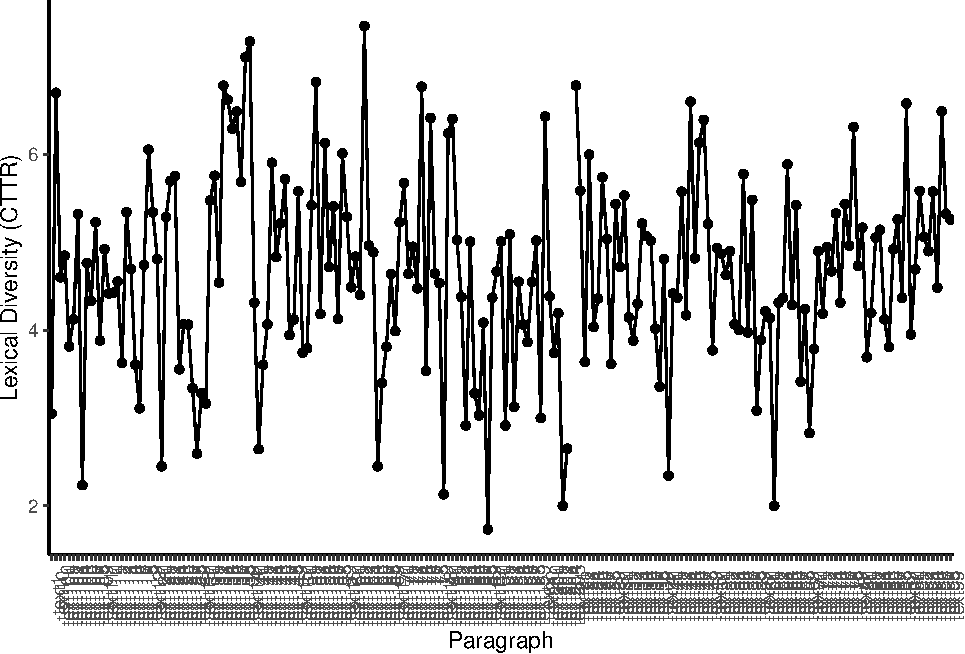
\includegraphics{_main_files/figure-latex/ggplot-lexdiv-1.pdf}

Another thing we can do is look at the similarities and distances between documents. With this, we can answer questions such as: how \emph{different} are these documents from each other? And if different (or similar), how different (or similar)? The idea is that the larger the similarity is, the smaller the distance is as well. A good way to understand the idea of similarity is to consider how many operations you need to perform to change one text into the other. The more ``replace'' options you have to carry out, the more different the text. As for the distances, it is best to consider the texts as having positions on a Cartesian plane (with positions based on their word counts). The distance between these two points (either Euclidean, Manhattan or other) is then the distance between the texts.

Let's start with a look at these similarities (note again that there are many different methods to calculate this):

\begin{Shaded}
\begin{Highlighting}[]
\NormalTok{corpus\_similarties }\OtherTok{\textless{}{-}} \FunctionTok{textstat\_simil}\NormalTok{(data\_dfm, }\AttributeTok{method =} \StringTok{"correlation"}\NormalTok{, }\AttributeTok{margin =} \StringTok{"documents"}\NormalTok{)}
\NormalTok{corpus\_similarties }\OtherTok{\textless{}{-}} \FunctionTok{as.data.frame}\NormalTok{(corpus\_similarties)}
\end{Highlighting}
\end{Shaded}

Note that while we look here at the documents, we could also look at individual words (set \texttt{margin="features}). For now, let us look at the distances between the documents, choosing the Euclidean distance between the documents as our metric:

\begin{Shaded}
\begin{Highlighting}[]
\NormalTok{corpus\_distances }\OtherTok{\textless{}{-}} \FunctionTok{textstat\_dist}\NormalTok{(data\_dfm, }\AttributeTok{margin =} \StringTok{"documents"}\NormalTok{, }\AttributeTok{method =} \StringTok{"euclidean"}\NormalTok{)}
\NormalTok{corpus\_distances\_df }\OtherTok{\textless{}{-}} \FunctionTok{as.data.frame}\NormalTok{(corpus\_distances)}
\end{Highlighting}
\end{Shaded}

If we want to, we can even convert this data into a dendrogram. We do this by taking the information on the distances out of the \texttt{corpus\_distances} object, make them into a triangular matrix, and plot them:

\begin{Shaded}
\begin{Highlighting}[]
\FunctionTok{plot}\NormalTok{(}\FunctionTok{hclust}\NormalTok{(}\FunctionTok{as.dist}\NormalTok{(corpus\_distances)), }\AttributeTok{hang =} \SpecialCharTok{{-}}\DecValTok{1}\NormalTok{)}
\end{Highlighting}
\end{Shaded}

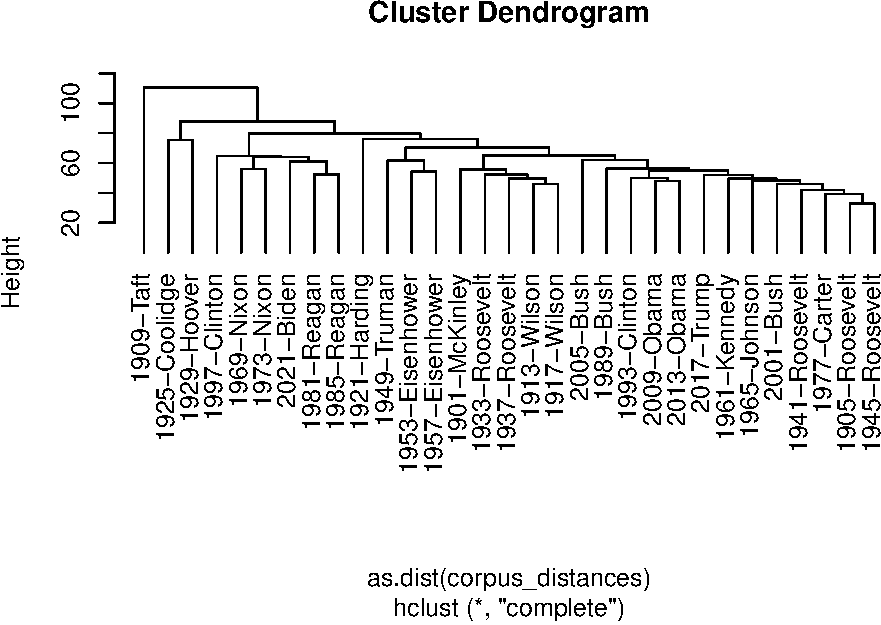
\includegraphics{_main_files/figure-latex/plot-distances-1.pdf}

Finally, let us look at the entropy of our texts. The entropy of a document measures the `amount' of information each letter of the text produces. To get an idea of what this means, consider the `e' is an often occurring letter in an English text, while `z' is not. Thus, a word with a `z' in it, it more unique and thus likely to carry unique and interesting information. The `higher' the entropy of a text, the less `information' is in it:

\begin{Shaded}
\begin{Highlighting}[]
\NormalTok{corpus\_entropy\_docs }\OtherTok{\textless{}{-}} \FunctionTok{textstat\_entropy}\NormalTok{(data\_dfm, }\StringTok{"documents"}\NormalTok{)}
\NormalTok{corpus\_entropy\_docs }\OtherTok{\textless{}{-}} \FunctionTok{as.data.frame}\NormalTok{(corpus\_entropy\_docs)}
\end{Highlighting}
\end{Shaded}

While not as common as the other distance metrics, entropy is sometimes used to measure the similarity between texts. Thus, it can be useful if we want to know the importance of certain words. This is because if a certain word is not important, we could consider it to be a stop word:

\begin{Shaded}
\begin{Highlighting}[]
\NormalTok{corpus\_entropy\_feats }\OtherTok{\textless{}{-}} \FunctionTok{textstat\_entropy}\NormalTok{(data\_dfm, }\StringTok{"features"}\NormalTok{)}
\NormalTok{corpus\_entropy\_feats }\OtherTok{\textless{}{-}} \FunctionTok{as.data.frame}\NormalTok{(corpus\_entropy\_feats)}
\NormalTok{corpus\_entropy\_feats }\OtherTok{\textless{}{-}}\NormalTok{ corpus\_entropy\_feats[}\FunctionTok{order}\NormalTok{(}\SpecialCharTok{{-}}\NormalTok{corpus\_entropy\_feats}\SpecialCharTok{$}\NormalTok{entropy),]}
\FunctionTok{head}\NormalTok{(corpus\_entropy\_feats, }\DecValTok{10}\NormalTok{)}
\end{Highlighting}
\end{Shaded}

\begin{verbatim}
##       feature  entropy
## 8      soviet 6.620700
## 2         war 6.443909
## 9       union 6.081728
## 7      states 5.923134
## 6      united 5.823699
## 57   military 5.612866
## 1        cold 5.573738
## 107 communist 5.374768
## 222        us 5.293932
## 12    western 5.289149
\end{verbatim}

Looking at the data, we find that `soviet', `war' and `union' have pretty high entropies. This indicates that the words added little to the information of the documents, and would-be candidates for removal from our corpus.

\chapter{Dictionary Analysis}\label{dictionary-analysis}

One of the simplest forms of quantitative text analysis is dictionary analysis. The idea here is to look at the rate at which keywords appear in a text to classify documents into categories. Also, we can measure the extent to which documents belong to particular categories. As we do so without making any assumptions, dictionary methods present a non-statistical to text analysis. A well-known example is measuring the tone in newspaper articles, speeches, children's writings, and so on by using sentiment analysis dictionaries. Another example is the measuring of policy content in different documents as illustrated by the Policy Agendas Project dictionary (\citeproc{ref-Albaugh2013a}{Albaugh et al., 2013}).

Here, we will carry out three such analyses, the first a standard analysis and the other two focusing on sentiment. For the former, we will use political party manifestos, while for the latter we will use movie reviews and Twitter data.

\section{Classical Dictionary Analysis}\label{classical-dictionary-analysis}

As for our dictionaries, we can either make the dictionary ourselves or use an off-the-shelf version. For the latter, we can either import the files we already have into R or use some of the versions that come with the \texttt{quanteda.dictionaries} package. For this, we first load the package:

\begin{Shaded}
\begin{Highlighting}[]
\FunctionTok{library}\NormalTok{(quanteda.dictionaries)}
\end{Highlighting}
\end{Shaded}

We then apply one of these dictionaries to the document feature matrix we in the previous chapter. As a dictionary, we will use the one made by Laver \& Garry (\citeproc{ref-Laver2000a}{2000}), meant for estimating policy positions from political texts. We first load this dictionary into R and then run it on the dfm using the \texttt{dfm\_lookup} command:

\begin{Shaded}
\begin{Highlighting}[]
\NormalTok{data\_dictionary\_LaverGarry}
\NormalTok{dictionary\_results }\OtherTok{\textless{}{-}} \FunctionTok{dfm\_lookup}\NormalTok{(data\_dfm, data\_dictionary\_LaverGarry)}
\NormalTok{dictionary\_results}
\end{Highlighting}
\end{Shaded}

Apart from off-the-shelf dictionaries, it is also possible to create our own which could suit our research question better. One approach is to use prior theory to come up with different categories and their associated words. Another approach is to use reference texts to come up with categories and words. We can also combine different dictionaries as illustrated by Young \& Soroka (\citeproc{ref-Young2012a}{2012}), or different dictionaries and keywords from categories in a manual coding scheme (\citeproc{ref-Lind2019a}{Lind et al., 2019}). Finally, we can use expert or crowd coding assessments to determine the words that best match different categories in a dictionary (\citeproc{ref-Haselmayer2017a}{Haselmayer \& Jenny, 2017}).

If we want to create our own dictionary in \texttt{quanteda} we use the same commands as above, but we first have to create the dictionary. To do so, we specify the words in a named list. This list contains keys (the words we want to look for) and the categories to which they belong. We then transform this list into a dictionary. Here, we choose some words which we believe will allow us to identify the different parties with ease:

\begin{Shaded}
\begin{Highlighting}[]
\NormalTok{dic\_list }\OtherTok{\textless{}{-}} \FunctionTok{list}\NormalTok{(}\AttributeTok{economy =} \FunctionTok{c}\NormalTok{(}\StringTok{"tax*"}\NormalTok{, }\StringTok{"invest*"}\NormalTok{, }\StringTok{"trade"}\NormalTok{), }
                 \AttributeTok{war =} \FunctionTok{c}\NormalTok{(}\StringTok{"army"}\NormalTok{, }\StringTok{"troops"}\NormalTok{, }\StringTok{"fight"}\NormalTok{), }
                 \AttributeTok{diplomacy =} \FunctionTok{c}\NormalTok{(}\StringTok{"nato"}\NormalTok{,}\StringTok{"comintern"}\NormalTok{,}\StringTok{"un"}\NormalTok{), }
                 \AttributeTok{government =} \FunctionTok{c}\NormalTok{(}\StringTok{"washington"}\NormalTok{,}\StringTok{"moscow"}\NormalTok{,}\StringTok{"beijing"}\NormalTok{)}
\NormalTok{                 )}

\NormalTok{dic\_created }\OtherTok{\textless{}{-}} \FunctionTok{dictionary}\NormalTok{(dic\_list, }\AttributeTok{tolower =} \ConstantTok{FALSE}\NormalTok{)}
\NormalTok{dic\_created}
\end{Highlighting}
\end{Shaded}

\begin{verbatim}
## Dictionary object with 4 key entries.
## - [economy]:
##   - tax*, invest*, trade
## - [war]:
##   - army, troops, fight
## - [diplomacy]:
##   - nato, comintern, un
## - [government]:
##   - washington, moscow, beijing
\end{verbatim}

If you compare the \texttt{dic\_list} file with the \texttt{data\_dictionary\_LaverGarry} file, you will find that it has the same structure. To see the result, we can use the same command:

\begin{Shaded}
\begin{Highlighting}[]
\NormalTok{dictionary\_created }\OtherTok{\textless{}{-}} \FunctionTok{dfm\_lookup}\NormalTok{(data\_dfm, dic\_created)}
\NormalTok{dictionary\_created}
\end{Highlighting}
\end{Shaded}

\begin{verbatim}
## Document-feature matrix of: 205 documents, 4 features (89.39% sparse) and 0 docvars.
##        features
## docs    economy war diplomacy government
##   text1       0   0         0          0
##   text2       0   0         0          0
##   text3       0   0         0          0
##   text4       0   0         0          0
##   text5       0   0         0          0
##   text6       0   0         0          0
## [ reached max_ndoc ... 199 more documents ]
\end{verbatim}

Also note that if you would like to convert this dfm into a regular dataframe, you can use the \texttt{convert} command included in \texttt{quanteda}:

\begin{Shaded}
\begin{Highlighting}[]
\NormalTok{dictionary\_df }\OtherTok{\textless{}{-}} \FunctionTok{convert}\NormalTok{(dictionary\_created, }\AttributeTok{to =} \StringTok{"data.frame"}\NormalTok{)}
\end{Highlighting}
\end{Shaded}

Moreover, while we could look at this dataframe by either calling it in the console or looking at it in the Environment, we can also make it into an HTML widget, using the \texttt{DT} and \texttt{data.table} packages:

\begin{Shaded}
\begin{Highlighting}[]
\NormalTok{DT}\SpecialCharTok{::}\FunctionTok{datatable}\NormalTok{(dictionary\_df)}
\end{Highlighting}
\end{Shaded}

\begin{verbatim}
## PhantomJS not found. You can install it with webshot::install_phantomjs(). If it is installed, please make sure the phantomjs executable can be found via the PATH variable.
\end{verbatim}

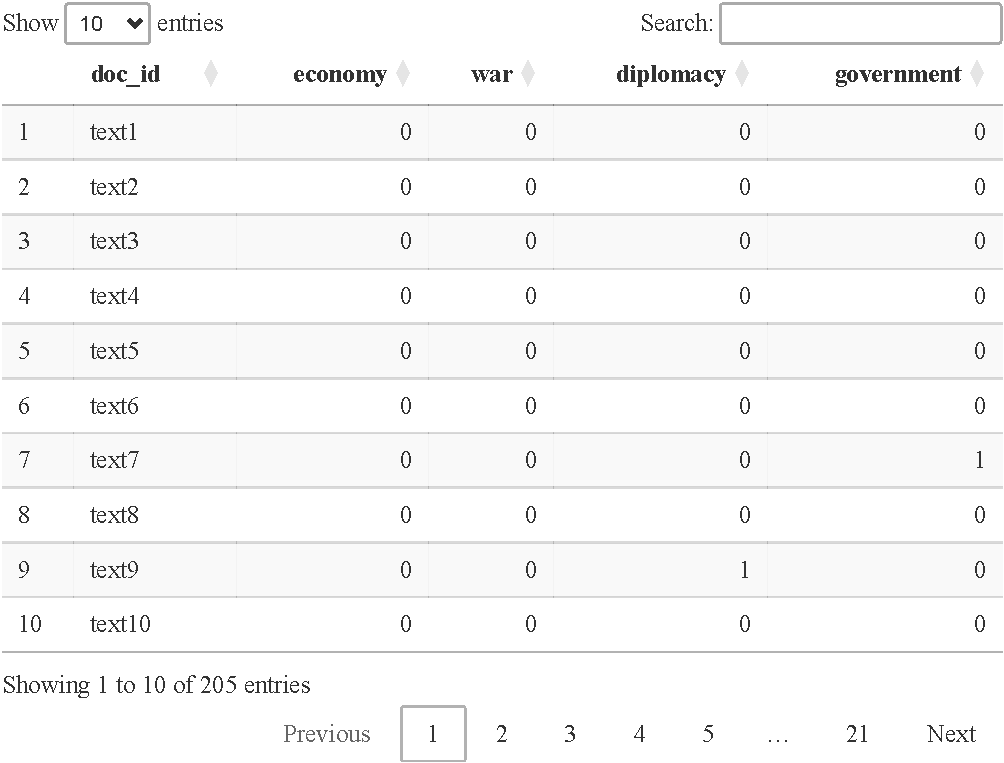
\includegraphics{_main_files/figure-latex/datatable-owndictionary-1.pdf}

\section{Sentiment Analysis}\label{sentiment-analysis}

The logic of dictionaries is that we can use them to see which kind of topics are present in our documents. Yet, we can also use them to provide us with measurements that are most often related to scaling. One way to do so is with \emph{sentiment analysis}. Here, we look at whether a certain piece of text is happy, angry, positive, negative, and so on. One case in which this can help us is with movie reviews. These reviews give us a description of a movie and then tell us their opinion. Another is when we look at Twitter data, to capture the `mood of the moment'. Here, we will look at both, starting with the movie reviews.

\subsection{Movie Reviews}\label{movie-reviews}

First, we load some reviews into R. The corpus we use here contains 50,000 movie reviews, each with a 1-10 rating (amongst others). As 50,000 reviews make the analysis quite slow, we will first select 30 reviews at random from this corpus. We do so via \texttt{corpus\_sample}, after which we transform it via a tokens object into a dfm:

\begin{Shaded}
\begin{Highlighting}[]
\FunctionTok{library}\NormalTok{(quanteda.classifiers)}
\NormalTok{reviews }\OtherTok{\textless{}{-}} \FunctionTok{corpus\_sample}\NormalTok{(data\_corpus\_LMRD, }\DecValTok{30}\NormalTok{)}
\NormalTok{reviews\_tokens }\OtherTok{\textless{}{-}} \FunctionTok{tokens}\NormalTok{(reviews)}
\NormalTok{reviews\_dfm }\OtherTok{\textless{}{-}} \FunctionTok{dfm}\NormalTok{(reviews\_tokens)}
\end{Highlighting}
\end{Shaded}

The next step is to load in a sentiment analysis dictionary. Here, we will use the Lexicoder Sentiment Dictionary, included in \texttt{quanteda} and run it on the dfm:

\begin{Shaded}
\begin{Highlighting}[]
\NormalTok{data\_dictionary\_LSD2015}
\NormalTok{results\_dfm }\OtherTok{\textless{}{-}} \FunctionTok{dfm\_lookup}\NormalTok{(reviews\_dfm, data\_dictionary\_LSD2015)}
\NormalTok{results\_dfm}
\end{Highlighting}
\end{Shaded}

The next step is to convert the results to a data frame and view them:

\begin{Shaded}
\begin{Highlighting}[]
\NormalTok{sentiment }\OtherTok{\textless{}{-}} \FunctionTok{convert}\NormalTok{(results\_dfm, }\AttributeTok{to=}\StringTok{"data.frame"}\NormalTok{)}
\FunctionTok{head}\NormalTok{(sentiment)}
\end{Highlighting}
\end{Shaded}

\begin{verbatim}
##                 doc_id negative positive neg_positive neg_negative
## 1  test/neg/2033_3.txt        2        5            0            0
## 2 train/neg/1884_3.txt        6        2            0            0
## 3 train/neg/2221_1.txt       15        7            0            0
## 4  test/neg/8691_1.txt       15       12            0            0
## 5  train/neg/824_3.txt       15        6            0            0
## 6  test/pos/4257_9.txt        2        1            0            0
\end{verbatim}

Since movie reviews usually come with some sort of rating (often in the form of stars), we can see if this relates to the sentiment of the review. To do so, we have to take the rating out of the dfm and place it in a new data frame with the positive and negative sentiments:

\begin{Shaded}
\begin{Highlighting}[]
\NormalTok{star\_data }\OtherTok{\textless{}{-}}\NormalTok{ reviews\_dfm}\SpecialCharTok{@}\NormalTok{docvars}\SpecialCharTok{$}\NormalTok{rating}
\NormalTok{stargraph }\OtherTok{\textless{}{-}} \FunctionTok{as.data.frame}\NormalTok{(}\FunctionTok{cbind}\NormalTok{(star\_data, sentiment}\SpecialCharTok{$}\NormalTok{negative, sentiment}\SpecialCharTok{$}\NormalTok{positive))}
\FunctionTok{names}\NormalTok{(stargraph) }\OtherTok{\textless{}{-}} \FunctionTok{c}\NormalTok{(}\StringTok{"stars"}\NormalTok{,}\StringTok{"negative"}\NormalTok{,}\StringTok{"positive"}\NormalTok{)}
\end{Highlighting}
\end{Shaded}

To compare the sentiment with the stars, we first have to combine the senitments into a scale. Of the many ways to do so, the simplest is to take the difference between the positive and negative words (positive -- negative). Another option is to take the ratio of positive words against both positive and negative (positive/positive+negative). Here, we do both:

\begin{Shaded}
\begin{Highlighting}[]
\NormalTok{sentiment\_difference }\OtherTok{\textless{}{-}}\NormalTok{ stargraph}\SpecialCharTok{$}\NormalTok{positive}\SpecialCharTok{{-}}\NormalTok{stargraph}\SpecialCharTok{$}\NormalTok{negative}
\NormalTok{sentiment\_ratio }\OtherTok{\textless{}{-}}\NormalTok{ (stargraph}\SpecialCharTok{$}\NormalTok{positive}\SpecialCharTok{/}\NormalTok{ (stargraph}\SpecialCharTok{$}\NormalTok{positive }\SpecialCharTok{+}\NormalTok{ stargraph}\SpecialCharTok{$}\NormalTok{negative))}
\NormalTok{stargraph }\OtherTok{\textless{}{-}} \FunctionTok{cbind}\NormalTok{(stargraph, sentiment\_difference,sentiment\_ratio)}
\end{Highlighting}
\end{Shaded}

Then, we can plot the ratings and the scaled sentiment measures together with a linear regression line:

\begin{Shaded}
\begin{Highlighting}[]
\FunctionTok{library}\NormalTok{(ggplot2)}

\FunctionTok{ggplot}\NormalTok{(stargraph,}\FunctionTok{aes}\NormalTok{(}\AttributeTok{x =}\NormalTok{ sentiment\_difference, }\AttributeTok{y =}\NormalTok{ stars)) }\SpecialCharTok{+}
 \FunctionTok{geom\_point}\NormalTok{(}\AttributeTok{shape =} \DecValTok{1}\NormalTok{) }\SpecialCharTok{+}
 \FunctionTok{geom\_smooth}\NormalTok{(}\AttributeTok{method =}\NormalTok{ lm, }\AttributeTok{se =} \ConstantTok{FALSE}\NormalTok{, }\AttributeTok{color=}\StringTok{"black"}\NormalTok{) }\SpecialCharTok{+}
 \FunctionTok{scale\_y\_continuous}\NormalTok{(}\AttributeTok{limits =} \FunctionTok{c}\NormalTok{(}\DecValTok{0}\NormalTok{, }\FloatTok{10.5}\NormalTok{), }\AttributeTok{expand =} \FunctionTok{c}\NormalTok{(}\DecValTok{0}\NormalTok{,}\DecValTok{0}\NormalTok{))}\SpecialCharTok{+}
 \FunctionTok{xlab}\NormalTok{(}\StringTok{"Positive minus Negative"}\NormalTok{) }\SpecialCharTok{+}
 \FunctionTok{ylab}\NormalTok{(}\StringTok{"Stars"}\NormalTok{) }\SpecialCharTok{+}
 \FunctionTok{theme\_classic}\NormalTok{()}
\end{Highlighting}
\end{Shaded}

\begin{verbatim}
## `geom_smooth()` using formula = 'y ~ x'
\end{verbatim}

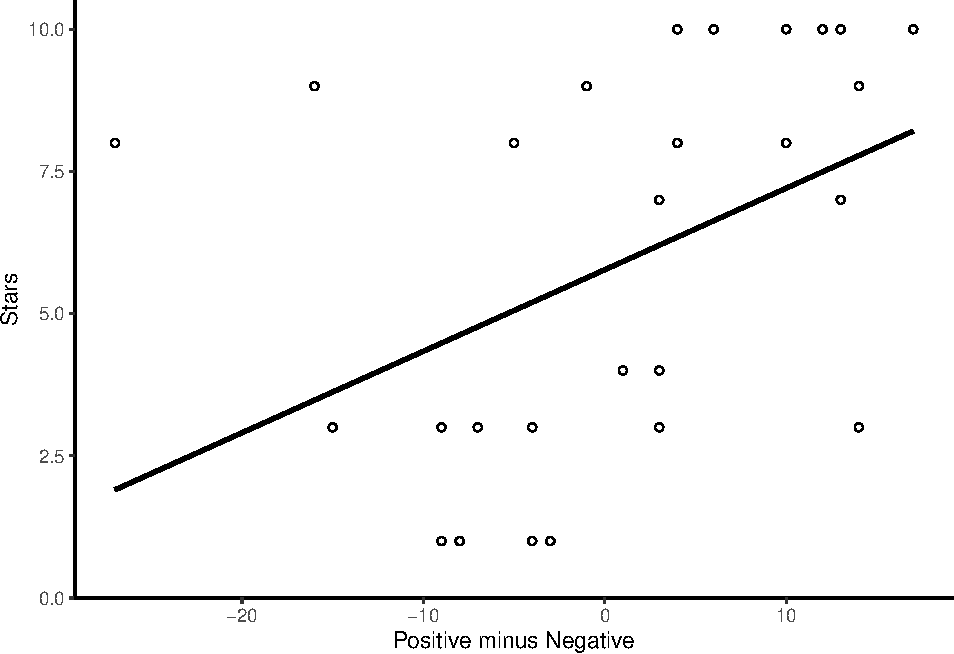
\includegraphics{_main_files/figure-latex/ggplot-moviereviews-posmin-1.pdf}

\begin{Shaded}
\begin{Highlighting}[]
\FunctionTok{ggplot}\NormalTok{(stargraph,}\FunctionTok{aes}\NormalTok{(}\AttributeTok{x =}\NormalTok{ sentiment\_ratio, }\AttributeTok{y =}\NormalTok{ stars)) }\SpecialCharTok{+}
 \FunctionTok{geom\_point}\NormalTok{(}\AttributeTok{shape =} \DecValTok{1}\NormalTok{) }\SpecialCharTok{+}
 \FunctionTok{geom\_smooth}\NormalTok{(}\AttributeTok{method =}\NormalTok{ lm, }\AttributeTok{se =} \ConstantTok{FALSE}\NormalTok{, }\AttributeTok{color=}\StringTok{"black"}\NormalTok{) }\SpecialCharTok{+}
 \FunctionTok{scale\_y\_continuous}\NormalTok{(}\AttributeTok{limits =} \FunctionTok{c}\NormalTok{(}\DecValTok{0}\NormalTok{, }\FloatTok{10.5}\NormalTok{), }\AttributeTok{expand =} \FunctionTok{c}\NormalTok{(}\DecValTok{0}\NormalTok{,}\DecValTok{0}\NormalTok{))}\SpecialCharTok{+}
 \FunctionTok{scale\_x\_continuous}\NormalTok{(}\AttributeTok{limits =} \FunctionTok{c}\NormalTok{(}\DecValTok{0}\NormalTok{, }\DecValTok{1}\NormalTok{), }\AttributeTok{expand =} \FunctionTok{c}\NormalTok{(}\DecValTok{0}\NormalTok{,}\DecValTok{0}\NormalTok{))}\SpecialCharTok{+}
 \FunctionTok{xlab}\NormalTok{(}\StringTok{"Ratio of Positive to Total"}\NormalTok{) }\SpecialCharTok{+}
 \FunctionTok{ylab}\NormalTok{(}\StringTok{"Stars"}\NormalTok{) }\SpecialCharTok{+}
 \FunctionTok{theme\_classic}\NormalTok{()}
\end{Highlighting}
\end{Shaded}

\begin{verbatim}
## `geom_smooth()` using formula = 'y ~ x'
\end{verbatim}

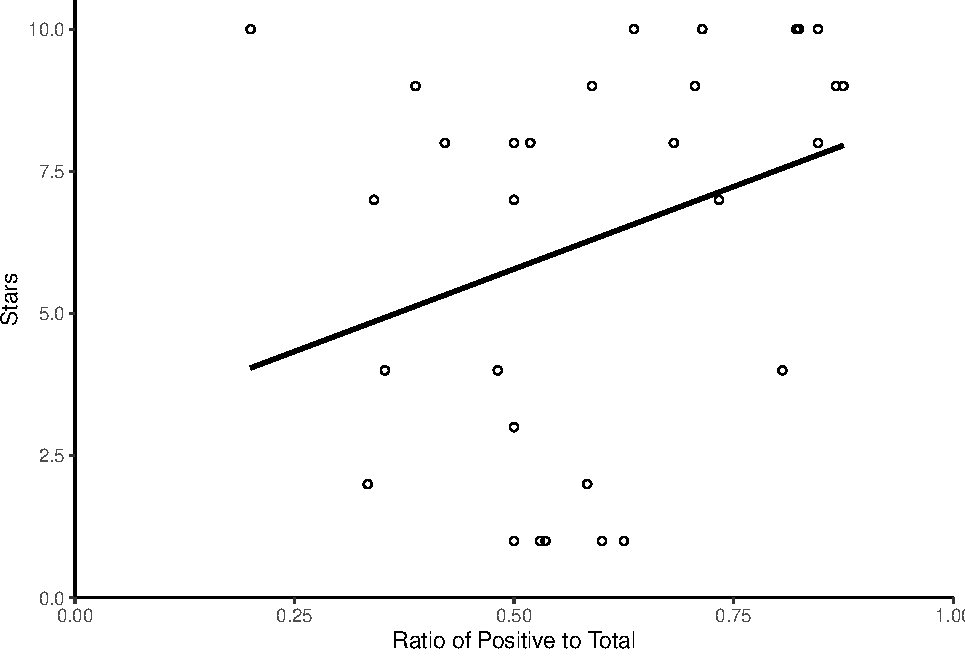
\includegraphics{_main_files/figure-latex/ggplot-moviereviews-stars-1.pdf}

Finally, let us look at how we can make any more inferences, by estimating confidence intervals around the point estimates. For this, we again add a column, this time one with the total of positive and negative words as scored by the dictionary. We do so by copying the data frame to a new data frame and adding a new column filled with NA values:

\begin{Shaded}
\begin{Highlighting}[]
\NormalTok{reviews\_bootstrap }\OtherTok{\textless{}{-}}\NormalTok{ sentiment}
\NormalTok{reviews\_bootstrap}\SpecialCharTok{$}\NormalTok{n }\OtherTok{\textless{}{-}} \ConstantTok{NA}
\end{Highlighting}
\end{Shaded}

We then again specify the number of reviews, the replications that we want and change the data frame into an array:

\begin{Shaded}
\begin{Highlighting}[]
\FunctionTok{library}\NormalTok{(combinat)}

\NormalTok{nman }\OtherTok{\textless{}{-}} \FunctionTok{nrow}\NormalTok{(reviews\_bootstrap)}
\NormalTok{nrepl }\OtherTok{\textless{}{-}} \DecValTok{1000}
\NormalTok{manifBSn }\OtherTok{\textless{}{-}}\NormalTok{ manifBSnRand }\OtherTok{\textless{}{-}} \FunctionTok{array}\NormalTok{(}\FunctionTok{as.matrix}\NormalTok{(reviews\_bootstrap[,}\DecValTok{2}\SpecialCharTok{:}\DecValTok{3}\NormalTok{]),}
 \FunctionTok{c}\NormalTok{(nman, }\DecValTok{2}\NormalTok{, nrepl }\SpecialCharTok{+} \DecValTok{1}\NormalTok{), }
 \AttributeTok{dimnames =} \FunctionTok{list}\NormalTok{(}\DecValTok{1}\SpecialCharTok{:}\NormalTok{nman,}\FunctionTok{names}\NormalTok{(reviews\_bootstrap[,}\DecValTok{2}\SpecialCharTok{:}\DecValTok{3}\NormalTok{]), }
 \DecValTok{0}\SpecialCharTok{:}\NormalTok{nrepl))}
\end{Highlighting}
\end{Shaded}

Then, we bootstrap the word counts for each movie review and compute percentages for each category using a multinomial draw:

\begin{Shaded}
\begin{Highlighting}[]
\NormalTok{n }\OtherTok{\textless{}{-}} \FunctionTok{apply}\NormalTok{(manifBSn[}\DecValTok{1}\SpecialCharTok{:}\FunctionTok{nrow}\NormalTok{(manifBSn), , }\DecValTok{1}\NormalTok{], }\DecValTok{1}\NormalTok{, sum)}
\NormalTok{p }\OtherTok{\textless{}{-}}\NormalTok{ manifBSn[, , }\DecValTok{1}\NormalTok{]}\SpecialCharTok{/}\NormalTok{n}

\ControlFlowTok{for}\NormalTok{(i }\ControlFlowTok{in} \DecValTok{1}\SpecialCharTok{:}\NormalTok{nrepl) \{}
\NormalTok{ manifBSn[, , i] }\OtherTok{\textless{}{-}} \FunctionTok{rmultinomial}\NormalTok{(n, p)}
\NormalTok{ \}}
\end{Highlighting}
\end{Shaded}

We can then ask R to compute the quantities of interest. These are standard errors for each category, as well as the percentage coded for each category (\citeproc{ref-Mikhaylov2012a}{Mikhaylov et al., 2012}):

\begin{Shaded}
\begin{Highlighting}[]
\NormalTok{NegativeSE }\OtherTok{\textless{}{-}} \FunctionTok{apply}\NormalTok{(manifBSn[, }\StringTok{"negative"}\NormalTok{, ]}\SpecialCharTok{/}\NormalTok{n }\SpecialCharTok{*} \DecValTok{100}\NormalTok{, }\DecValTok{1}\NormalTok{, sd)}
\NormalTok{PositiveSE }\OtherTok{\textless{}{-}} \FunctionTok{apply}\NormalTok{(manifBSn[, }\StringTok{"positive"}\NormalTok{, ]}\SpecialCharTok{/}\NormalTok{n }\SpecialCharTok{*} \DecValTok{100}\NormalTok{, }\DecValTok{1}\NormalTok{, sd)}
\NormalTok{perNegative }\OtherTok{\textless{}{-}} \FunctionTok{apply}\NormalTok{(manifBSn[, }\StringTok{"negative"}\NormalTok{, ]}\SpecialCharTok{/}\NormalTok{n }\SpecialCharTok{*} \DecValTok{100}\NormalTok{, }\DecValTok{1}\NormalTok{, mean)}
\NormalTok{perPositive }\OtherTok{\textless{}{-}} \FunctionTok{apply}\NormalTok{(manifBSn[, }\StringTok{"positive"}\NormalTok{, ]}\SpecialCharTok{/}\NormalTok{n }\SpecialCharTok{*} \DecValTok{100}\NormalTok{, }\DecValTok{1}\NormalTok{, mean)}
\end{Highlighting}
\end{Shaded}

We then save these quantities of interest in a new data frame:

\begin{Shaded}
\begin{Highlighting}[]
\NormalTok{dataBS }\OtherTok{\textless{}{-}} \FunctionTok{data.frame}\NormalTok{(}\FunctionTok{cbind}\NormalTok{(reviews\_bootstrap[, }\DecValTok{1}\SpecialCharTok{:}\DecValTok{3}\NormalTok{], NegativeSE,PositiveSE, perNegative, perPositive))}
\end{Highlighting}
\end{Shaded}

Then, we first calculate the confidence intervals and add these:

\begin{Shaded}
\begin{Highlighting}[]
\NormalTok{pos\_hi }\OtherTok{\textless{}{-}}\NormalTok{ dataBS}\SpecialCharTok{$}\NormalTok{perPositive }\SpecialCharTok{+}\NormalTok{ (}\FloatTok{1.96} \SpecialCharTok{*}\NormalTok{ dataBS}\SpecialCharTok{$}\NormalTok{PositiveSE)}
\NormalTok{pos\_lo }\OtherTok{\textless{}{-}}\NormalTok{ dataBS}\SpecialCharTok{$}\NormalTok{perPositive }\SpecialCharTok{{-}}\NormalTok{ (}\FloatTok{1.96} \SpecialCharTok{*}\NormalTok{ dataBS}\SpecialCharTok{$}\NormalTok{PositiveSE)}
\NormalTok{neg\_lo }\OtherTok{\textless{}{-}}\NormalTok{ dataBS}\SpecialCharTok{$}\NormalTok{perNegative }\SpecialCharTok{{-}}\NormalTok{ (}\FloatTok{1.96} \SpecialCharTok{*}\NormalTok{ dataBS}\SpecialCharTok{$}\NormalTok{NegativeSE)}
\NormalTok{neg\_hi }\OtherTok{\textless{}{-}}\NormalTok{ dataBS}\SpecialCharTok{$}\NormalTok{perNegative }\SpecialCharTok{+}\NormalTok{ (}\FloatTok{1.96} \SpecialCharTok{*}\NormalTok{ dataBS}\SpecialCharTok{$}\NormalTok{NegativeSE)}
\NormalTok{dataBS }\OtherTok{\textless{}{-}} \FunctionTok{cbind}\NormalTok{(dataBS, pos\_hi, pos\_lo, neg\_lo, neg\_hi)}
\end{Highlighting}
\end{Shaded}

Finally, we can then make the graph. Here, we plot each of the positive and negative points and then overlay them with their error bars:

\begin{Shaded}
\begin{Highlighting}[]
\FunctionTok{library}\NormalTok{(ggplot2)}

\FunctionTok{ggplot}\NormalTok{() }\SpecialCharTok{+}
 \FunctionTok{geom\_point}\NormalTok{(}\AttributeTok{data =}\NormalTok{ dataBS,}\FunctionTok{aes}\NormalTok{(}\AttributeTok{x =}\NormalTok{ perPositive, }\AttributeTok{y =}\NormalTok{ doc\_id), }\AttributeTok{shape =} \DecValTok{0}\NormalTok{) }\SpecialCharTok{+}
 \FunctionTok{geom\_point}\NormalTok{(}\AttributeTok{data =}\NormalTok{ dataBS,}\FunctionTok{aes}\NormalTok{(}\AttributeTok{x =}\NormalTok{ perNegative, }\AttributeTok{y =}\NormalTok{ doc\_id), }\AttributeTok{shape =} \DecValTok{2}\NormalTok{) }\SpecialCharTok{+}
 \FunctionTok{geom\_errorbarh}\NormalTok{(}\AttributeTok{data =}\NormalTok{ dataBS,}\FunctionTok{aes}\NormalTok{(}\AttributeTok{x =}\NormalTok{ perPositive, }\AttributeTok{xmax =}\NormalTok{ pos\_hi,}\AttributeTok{xmin =}\NormalTok{ pos\_lo, }\AttributeTok{y =}\NormalTok{ doc\_id)) }\SpecialCharTok{+}
 \FunctionTok{geom\_errorbarh}\NormalTok{(}\AttributeTok{data =}\NormalTok{ dataBS,}\FunctionTok{aes}\NormalTok{(}\AttributeTok{x =}\NormalTok{ perNegative, }\AttributeTok{xmax =}\NormalTok{ neg\_hi,}\AttributeTok{xmin =}\NormalTok{ neg\_lo, }\AttributeTok{y =}\NormalTok{ doc\_id)) }\SpecialCharTok{+}
 \FunctionTok{xlab}\NormalTok{(}\StringTok{"Percent positive/negative with 95\% CIs"}\NormalTok{) }\SpecialCharTok{+}
 \FunctionTok{ylab}\NormalTok{(}\StringTok{"review"}\NormalTok{)}\SpecialCharTok{+}
 \FunctionTok{theme\_classic}\NormalTok{()}
\end{Highlighting}
\end{Shaded}

\begin{verbatim}
## Warning in geom_errorbarh(data = dataBS, aes(x = perPositive, xmax = pos_hi, :
## Ignoring unknown aesthetics: x
\end{verbatim}

\begin{verbatim}
## Warning in geom_errorbarh(data = dataBS, aes(x = perNegative, xmax = neg_hi, :
## Ignoring unknown aesthetics: x
\end{verbatim}

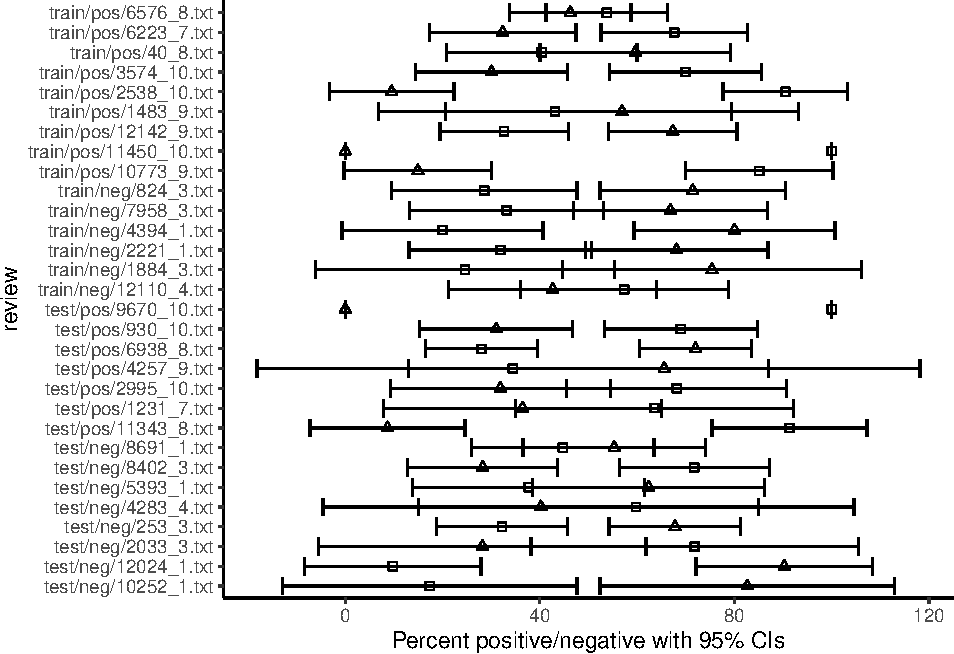
\includegraphics{_main_files/figure-latex/ggplot-moviereviews-posneg-1.pdf}

As we can see in this particular example, the fact that some documents are shorter than others introduces a lot of uncertainty in the estimates. As evident from the overlapping confidence intervals, for most reviews, the percentage of negative words is not very different from the percentage of positive words. In other words: the sentiment for these reviews is rather mixed.

\subsection{Twitter}\label{twitter}

Now, let us turn to an example using Twitter data. Here, we will look at the major problems that have occurred to several of the major US airlines. For this, researchers scraped data from Twitter between 16 and 24 February of 2015. Then, using the Crowdflower platform, they asked contributors to classify each tweet (their sentiment) as either negative, positive, or neutral, and, if negative, what their reason was for classifying it as such. Besides this, the data also contains information on how `confident' coders were about their classification and reason, some information on the Airline, and some info on the Tweet. Finally, we get some information on the ``gold'' tweets, which Crowdflower uses to figure out how well their coders are doing.

While we can download the data from the website (\url{https://www.kaggle.com/crowdflower/twitter-airline-sentiment}), for ease-of-use, we also placed it on GitHub:

\begin{Shaded}
\begin{Highlighting}[]
\NormalTok{urlfile }\OtherTok{=} \StringTok{"https://raw.githubusercontent.com/SCJBruinsma/qta{-}files/master/Tweets.csv"}
\NormalTok{tweets }\OtherTok{\textless{}{-}} \FunctionTok{read.csv}\NormalTok{(}\FunctionTok{url}\NormalTok{(urlfile))}
\end{Highlighting}
\end{Shaded}

Given that this is Twitter data, we have to do quite some cleaning to filter out everything we do not want. While we earlier saw that we can perform cleaning on a corpus, we can also clean our text while still in a data frame. We can do this with R's in-house \texttt{gsub} command, which can replace any part of a string. To understand how this works, say that we want to remove all the mentions of websites from our tweets. We then do as such:

\begin{Shaded}
\begin{Highlighting}[]
\NormalTok{tweets}\SpecialCharTok{$}\NormalTok{text }\OtherTok{\textless{}{-}} \FunctionTok{gsub}\NormalTok{(}\StringTok{"http.*"}\NormalTok{,}\StringTok{""}\NormalTok{, tweets}\SpecialCharTok{$}\NormalTok{text)}
\end{Highlighting}
\end{Shaded}

Thus, we substitute those strings that start with \texttt{http.*} (the asterisk denotes a wildcard, which means that anything can follow) and replace it with \texttt{} (that is, nothing). We do this for any string that is in \texttt{tweets\$text}. Using this technique, we also remove slashes, punctuation, various symbols, \texttt{RT} (retweets), and references (\texttt{href}):

\begin{Shaded}
\begin{Highlighting}[]
\NormalTok{tweets}\SpecialCharTok{$}\NormalTok{text }\OtherTok{\textless{}{-}} \FunctionTok{gsub}\NormalTok{(}\StringTok{"https.*"}\NormalTok{,}\StringTok{""}\NormalTok{, tweets}\SpecialCharTok{$}\NormalTok{text)}
\NormalTok{tweets}\SpecialCharTok{$}\NormalTok{text }\OtherTok{\textless{}{-}} \FunctionTok{gsub}\NormalTok{(}\StringTok{"}\SpecialCharTok{\textbackslash{}\textbackslash{}}\StringTok{$"}\NormalTok{, }\StringTok{""}\NormalTok{, tweets}\SpecialCharTok{$}\NormalTok{text) }
\NormalTok{tweets}\SpecialCharTok{$}\NormalTok{text }\OtherTok{\textless{}{-}} \FunctionTok{gsub}\NormalTok{(}\StringTok{"@}\SpecialCharTok{\textbackslash{}\textbackslash{}}\StringTok{w+"}\NormalTok{, }\StringTok{""}\NormalTok{, tweets}\SpecialCharTok{$}\NormalTok{text) }
\NormalTok{tweets}\SpecialCharTok{$}\NormalTok{text }\OtherTok{\textless{}{-}} \FunctionTok{gsub}\NormalTok{(}\StringTok{"[[:punct:]]"}\NormalTok{, }\StringTok{""}\NormalTok{, tweets}\SpecialCharTok{$}\NormalTok{text) }
\NormalTok{tweets}\SpecialCharTok{$}\NormalTok{text }\OtherTok{\textless{}{-}} \FunctionTok{gsub}\NormalTok{(}\StringTok{"[ |}\SpecialCharTok{\textbackslash{}t}\StringTok{]\{2,\}"}\NormalTok{, }\StringTok{""}\NormalTok{, tweets}\SpecialCharTok{$}\NormalTok{text) }
\NormalTok{tweets}\SpecialCharTok{$}\NormalTok{text }\OtherTok{\textless{}{-}} \FunctionTok{gsub}\NormalTok{(}\StringTok{"\^{} "}\NormalTok{, }\StringTok{""}\NormalTok{, tweets}\SpecialCharTok{$}\NormalTok{text) }
\NormalTok{tweets}\SpecialCharTok{$}\NormalTok{text }\OtherTok{\textless{}{-}} \FunctionTok{gsub}\NormalTok{(}\StringTok{" $"}\NormalTok{, }\StringTok{""}\NormalTok{, tweets}\SpecialCharTok{$}\NormalTok{text) }
\NormalTok{tweets}\SpecialCharTok{$}\NormalTok{text }\OtherTok{\textless{}{-}} \FunctionTok{gsub}\NormalTok{(}\StringTok{"RT"}\NormalTok{, }\StringTok{""}\NormalTok{, tweets}\SpecialCharTok{$}\NormalTok{text) }
\NormalTok{tweets}\SpecialCharTok{$}\NormalTok{text }\OtherTok{\textless{}{-}} \FunctionTok{gsub}\NormalTok{(}\StringTok{"href"}\NormalTok{, }\StringTok{""}\NormalTok{, tweets}\SpecialCharTok{$}\NormalTok{text)}
\end{Highlighting}
\end{Shaded}

We then transform our dataframe into a corpus (specifying that our text is in the \texttt{tweets\$text} field), transform this into a tokens object, lower all the words, remove the stop words, and finally make it into a dfm:

\begin{Shaded}
\begin{Highlighting}[]
\NormalTok{corpus\_tweets }\OtherTok{\textless{}{-}} \FunctionTok{corpus}\NormalTok{(tweets, }\AttributeTok{text\_field =} \StringTok{"text"}\NormalTok{)}
\NormalTok{data\_tweets\_tokens }\OtherTok{\textless{}{-}} \FunctionTok{tokens}\NormalTok{(corpus\_tweets)}
\NormalTok{data\_tweets\_tokens }\OtherTok{\textless{}{-}} \FunctionTok{tokens\_tolower}\NormalTok{(data\_tweets\_tokens, }\AttributeTok{keep\_acronyms =} \ConstantTok{TRUE}\NormalTok{)}
\NormalTok{data\_tweets\_tokens }\OtherTok{\textless{}{-}} \FunctionTok{tokens\_select}\NormalTok{(data\_tweets\_tokens, }\FunctionTok{stopwords}\NormalTok{(}\StringTok{"english"}\NormalTok{), }\AttributeTok{selection =} \StringTok{"remove"}\NormalTok{)}
\NormalTok{data\_tweets\_dfm }\OtherTok{\textless{}{-}} \FunctionTok{dfm}\NormalTok{(data\_tweets\_tokens)}
\end{Highlighting}
\end{Shaded}

Now we can apply our dictionary. We can do this in two ways: applying it to the dfm, or applying it to the tokens object. Both should give roughly similar results. Yet, given that \texttt{dfm\_lookup()} cannot detect multi-word expressions (as the dfm gets rid of all word order), we can use the \texttt{tokens\_lookup()} and then convert this into a dfm, to compensate for this. One reason to do this here is that the LSD2015 dictionary contains some multi-word expressions that \texttt{dfm\_lookup()} might miss. As a comparison, let us have a look at both:

\begin{Shaded}
\begin{Highlighting}[]
\NormalTok{results\_tokens }\OtherTok{\textless{}{-}} \FunctionTok{tokens\_lookup}\NormalTok{(data\_tweets\_tokens, data\_dictionary\_LSD2015)}
\NormalTok{results\_tokens }\OtherTok{\textless{}{-}} \FunctionTok{dfm}\NormalTok{(results\_tokens)}
\NormalTok{results\_tokens }\OtherTok{\textless{}{-}} \FunctionTok{convert}\NormalTok{(results\_tokens, }\AttributeTok{to=}\StringTok{"data.frame"}\NormalTok{)}

\NormalTok{results\_dfm }\OtherTok{\textless{}{-}} \FunctionTok{dfm\_lookup}\NormalTok{(data\_tweets\_dfm, data\_dictionary\_LSD2015)}
\NormalTok{results\_dfm }\OtherTok{\textless{}{-}} \FunctionTok{convert}\NormalTok{(results\_dfm, }\AttributeTok{to=}\StringTok{"data.frame"}\NormalTok{)}
\end{Highlighting}
\end{Shaded}

Now let us see how well our dictionary has done. To see this, we compare the sentiment of the tweet according to the dictionary with the sentiment assigned by the coder. We take this information out of our original data, and recode it (so it has got numerical values):

\begin{Shaded}
\begin{Highlighting}[]
\FunctionTok{library}\NormalTok{(car)}

\NormalTok{labels }\OtherTok{\textless{}{-}}\NormalTok{ tweets}\SpecialCharTok{$}\NormalTok{airline\_sentiment}
\NormalTok{labels }\OtherTok{\textless{}{-}}\NormalTok{ car}\SpecialCharTok{::}\FunctionTok{recode}\NormalTok{(labels, }\StringTok{"\textquotesingle{}positive\textquotesingle{}=1;\textquotesingle{}negative\textquotesingle{}={-}1;\textquotesingle{}neutral\textquotesingle{}=0"}\NormalTok{)}
\FunctionTok{table}\NormalTok{(labels)}
\end{Highlighting}
\end{Shaded}

A quick look at the data (with \texttt{table()}) reveals that the majority of the tweets are negative, a fair share neutral, and finally some positive ones. Now, let us bind this data to the output of our dictionary analysis, and calculate an overall score for each tweet. We do this by subtracting the positive score from the negative score (that is, the higher the score, the more positive the tweet):

\begin{Shaded}
\begin{Highlighting}[]
\NormalTok{comparison\_tokens }\OtherTok{\textless{}{-}} \FunctionTok{as.data.frame}\NormalTok{(}\FunctionTok{cbind}\NormalTok{(results\_tokens}\SpecialCharTok{$}\NormalTok{positive, results\_tokens}\SpecialCharTok{$}\NormalTok{negative, labels))}
\NormalTok{difference\_tokens }\OtherTok{\textless{}{-}}\NormalTok{ results\_tokens}\SpecialCharTok{$}\NormalTok{positive }\SpecialCharTok{{-}}\NormalTok{ results\_tokens}\SpecialCharTok{$}\NormalTok{negative}
\NormalTok{comparison\_tokens }\OtherTok{\textless{}{-}} \FunctionTok{cbind}\NormalTok{(comparison\_tokens, difference\_tokens)}

\NormalTok{comparison\_dfm }\OtherTok{\textless{}{-}} \FunctionTok{as.data.frame}\NormalTok{(}\FunctionTok{cbind}\NormalTok{(results\_dfm}\SpecialCharTok{$}\NormalTok{positive, results\_dfm}\SpecialCharTok{$}\NormalTok{negative, labels))}
\NormalTok{difference\_dfm }\OtherTok{\textless{}{-}}\NormalTok{ results\_dfm}\SpecialCharTok{$}\NormalTok{positive }\SpecialCharTok{{-}}\NormalTok{ results\_dfm}\SpecialCharTok{$}\NormalTok{negative}
\NormalTok{comparison\_dfm }\OtherTok{\textless{}{-}} \FunctionTok{cbind}\NormalTok{(comparison\_dfm, difference\_dfm)}
\end{Highlighting}
\end{Shaded}

Finally, we can place this all in a graph, in which we plot both the human judgement scores and the scores we calculated by subtracting the positive and negative codes. Also, we plot a simple linear equation to better understand the relation:

\begin{Shaded}
\begin{Highlighting}[]
\FunctionTok{library}\NormalTok{(ggplot2)}

\FunctionTok{ggplot}\NormalTok{(comparison\_tokens ,}\FunctionTok{aes}\NormalTok{(}\AttributeTok{x =}\NormalTok{ difference\_tokens, }\AttributeTok{y =}\NormalTok{ labels)) }\SpecialCharTok{+}
 \FunctionTok{geom\_jitter}\NormalTok{(}\AttributeTok{shape =} \DecValTok{1}\NormalTok{) }\SpecialCharTok{+}
 \FunctionTok{geom\_smooth}\NormalTok{(}\AttributeTok{method =}\NormalTok{ lm, }\AttributeTok{se =} \ConstantTok{FALSE}\NormalTok{) }\SpecialCharTok{+}
 \FunctionTok{xlab}\NormalTok{(}\StringTok{"Positive minus Negative"}\NormalTok{) }\SpecialCharTok{+}
 \FunctionTok{ylab}\NormalTok{(}\StringTok{"Human judgment"}\NormalTok{) }\SpecialCharTok{+}
 \FunctionTok{ggtitle}\NormalTok{(}\StringTok{"Using Tokens"}\NormalTok{)}\SpecialCharTok{+}
 \FunctionTok{theme\_classic}\NormalTok{()}
\end{Highlighting}
\end{Shaded}

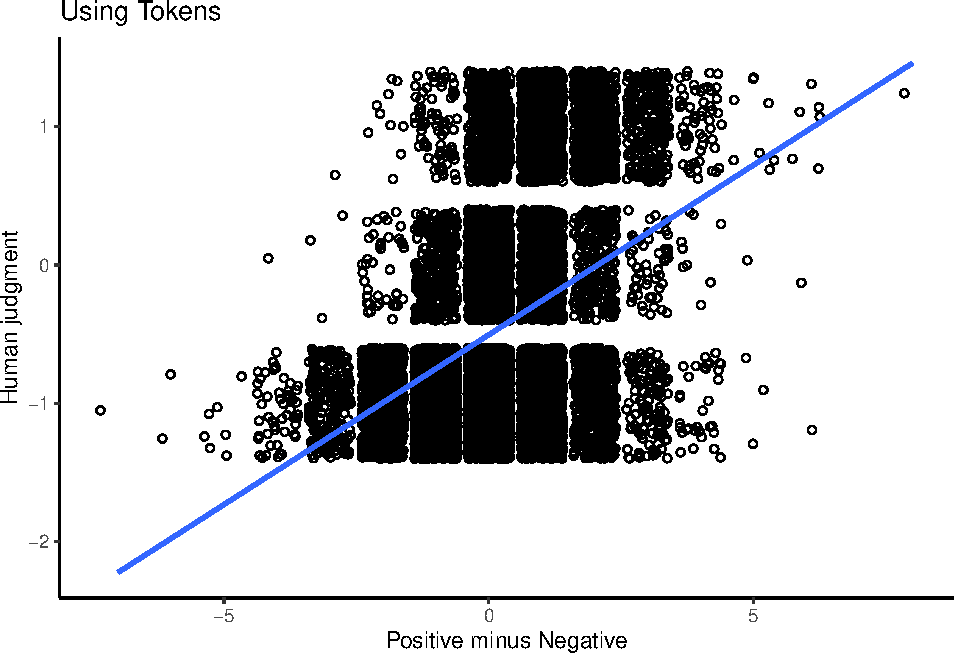
\includegraphics{_main_files/figure-latex/ggplot-tweets-tokensdfm-1.pdf}

\begin{Shaded}
\begin{Highlighting}[]
\FunctionTok{ggplot}\NormalTok{(comparison\_dfm, }\FunctionTok{aes}\NormalTok{(}\AttributeTok{x =}\NormalTok{ difference\_dfm, }\AttributeTok{y =}\NormalTok{ labels)) }\SpecialCharTok{+}
 \FunctionTok{geom\_jitter}\NormalTok{(}\AttributeTok{shape =} \DecValTok{1}\NormalTok{) }\SpecialCharTok{+}
 \FunctionTok{geom\_smooth}\NormalTok{(}\AttributeTok{method =}\NormalTok{ lm, }\AttributeTok{se =} \ConstantTok{FALSE}\NormalTok{) }\SpecialCharTok{+}
 \FunctionTok{xlab}\NormalTok{(}\StringTok{"Positive minus Negative"}\NormalTok{) }\SpecialCharTok{+}
 \FunctionTok{ylab}\NormalTok{(}\StringTok{"Human Judgment"}\NormalTok{) }\SpecialCharTok{+}
 \FunctionTok{ggtitle}\NormalTok{(}\StringTok{"Using DFM"}\NormalTok{)}\SpecialCharTok{+}
 \FunctionTok{theme\_classic}\NormalTok{()}
\end{Highlighting}
\end{Shaded}

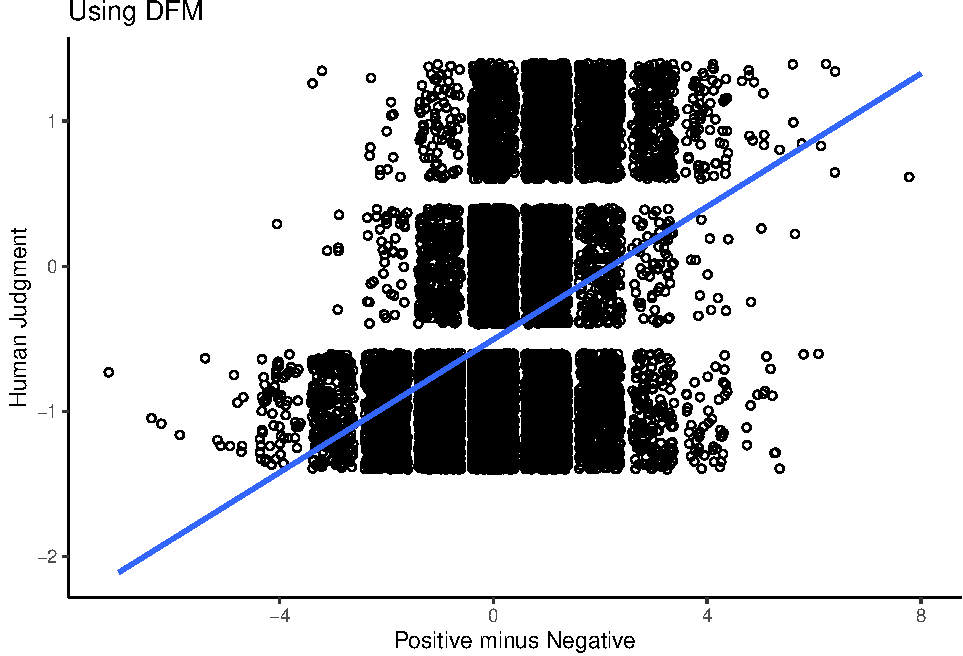
\includegraphics{_main_files/figure-latex/ggplot-tweets-tokensdfm-2.pdf}

As we can see, there is a positive relation (0.6947 for the tokens and 0.6914 for the dfm), which is quite good considering our approach does not involve any human coders at all.

\section{Sentiment Analysis using VADER}\label{sentiment-analysis-using-vader}

Another type of sentiment-analysis we can use is known as VADER Hutto \& Gilbert (\citeproc{ref-Hutto2014a}{2014}) (Valence Aware Dictionary and sEntiment Reasoner) which is a sentiment dictionary specifically made for sentiment in social media. Also, where most dictionaries tend to depend on a single coder classifying the terms, VADER uses multiple coders in order to arrive at a dictionary. So how well does it work? Let us test this again this the airline data we had before. First, we re-load this data back into R. Then, we separate the text and select 1000 tweets to work with:

\begin{Shaded}
\begin{Highlighting}[]
\NormalTok{urlfile }\OtherTok{=} \StringTok{"https://raw.githubusercontent.com/SCJBruinsma/qta{-}files/master/Tweets.csv"}
\NormalTok{tweets }\OtherTok{\textless{}{-}} \FunctionTok{read.csv}\NormalTok{(}\FunctionTok{url}\NormalTok{(urlfile))}
\NormalTok{tweets }\OtherTok{\textless{}{-}}\NormalTok{ tweets[}\FunctionTok{sample}\NormalTok{(}\FunctionTok{nrow}\NormalTok{(tweets), }\DecValTok{1000}\NormalTok{), ]}

\NormalTok{text }\OtherTok{\textless{}{-}}\NormalTok{ tweets}\SpecialCharTok{$}\NormalTok{text}
\end{Highlighting}
\end{Shaded}

We then apply VADER to our tweets. Note that the \texttt{vader} package has just two available commands: either to measure values for a single string, or to measure values for a dataframe. Here we will use the latter:

\begin{Shaded}
\begin{Highlighting}[]
\FunctionTok{library}\NormalTok{(vader)}
\NormalTok{results\_vader }\OtherTok{\textless{}{-}} \FunctionTok{vader\_df}\NormalTok{(text)}
\end{Highlighting}
\end{Shaded}

VADER then provides us with a dataframe consisting of seven different variables. The first contains the text, the second the ``word\_scores'' which is a string containing an ordered list with the scores for each of the words in the text, the third the ``compound'' which is the sum of all the valence scores in the document, and ``pos'', ``neg'' and ``neu'' refer to the positive, negative and neutral content specifically. In addition, there is an additional count for the occurrence of the word ``but'', as this often complicates the calculation of any type of sentiment.

To get a better idea of the output, we can look at the distribution of the scores:

\begin{Shaded}
\begin{Highlighting}[]
\FunctionTok{library}\NormalTok{(ggplot2)}

\FunctionTok{ggplot}\NormalTok{(}\AttributeTok{data =}\NormalTok{ results\_vader,}
       \FunctionTok{aes}\NormalTok{(}\AttributeTok{x=}\NormalTok{compound)}
\NormalTok{       ) }\SpecialCharTok{+} 
\FunctionTok{geom\_histogram}\NormalTok{(}\AttributeTok{bins =} \DecValTok{20}\NormalTok{,}
               \AttributeTok{color=}\StringTok{"black"}\NormalTok{,}
               \AttributeTok{fill=}\StringTok{"white"}\NormalTok{) }\SpecialCharTok{+}
\FunctionTok{theme\_classic}\NormalTok{()}
\end{Highlighting}
\end{Shaded}

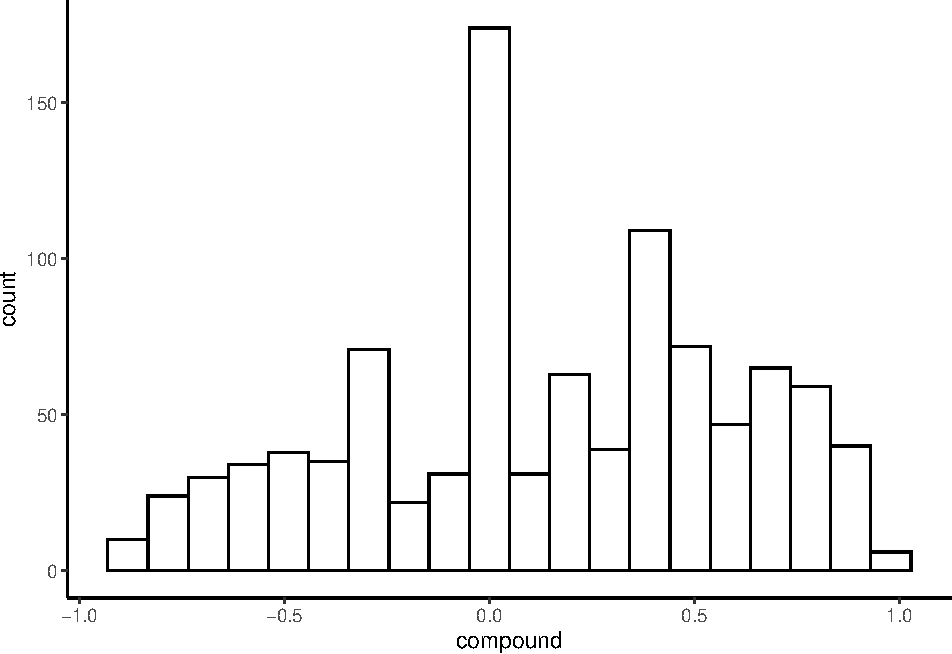
\includegraphics{_main_files/figure-latex/tweets-vader-outputs-1.pdf}

As we can see, there are quite a lot of neutral scores. If we look at the scores, tweets such as ``@JetBlue Counting on your flight 989 to get to DC!'' does not have any apparent sentiment, and seem to be quite often occurring, which most likely explains our results here.

\chapter{Exercices}\label{exercices}

\begin{enumerate}
\def\labelenumi{\arabic{enumi}.}
\tightlist
\item
  Using the sentiment analysis dictionary, see if you can estimate the sentiment of the Wikipedia article on the Cold War? Are there differences between the paragraphs, and if so, what causes them?
\item
  How did the Cold War influence culture? Make a dictionary with words measuring this and run it on the data to discuss this.
\end{enumerate}

\chapter{Scaling Methods}\label{scaling}

With a dictionary, we aimed to classify our texts into different categories based on the words they contain. While practical, there is no real way to compare these categories: one category is no better or worse than the other. If we do want to compare texts, we have to place them on some sort of scale. Here, we will look at three ways in which we can do so: \emph{Wordscores} (\citeproc{ref-Laver2003a}{Laver et al., 2003}), \emph{Wordfish} (\citeproc{ref-Slapin2008a}{Slapin \& Proksch, 2008}), and \emph{Correspondence Analysis}. The first two methods used to be part of the main \texttt{quanteda} package, but have now moved to the \texttt{quanteda.textmodels} package, while we find CA in the \texttt{FactoMineR} package.

\section{Wordscores}\label{wordscores}

The idea of Wordscores is to use reference texts (from which we know the position) to position our virgin texts (from which we do not know the position). Here, we aim to position the 2005 party manifestos of the five largest parties in the United Kingdom on a general left-right scale. For this, we will use the 2001 party manifestos of the same parties as reference texts. To know their positions, we will use the left-right scale from the 2002 \href{https://www.chesdata.eu/}{Chapel Hill Expert Survey} (\citeproc{ref-Bakker2012a}{Bakker et al., 2012}) to do so. So, we load our data, make a subset, transform it into a dfm, and clean it:

\begin{Shaded}
\begin{Highlighting}[]
\FunctionTok{library}\NormalTok{(quanteda)}
\FunctionTok{library}\NormalTok{(quanteda.corpora)}

\FunctionTok{data}\NormalTok{(data\_corpus\_ukmanifestos)}
\NormalTok{corpus\_manifestos }\OtherTok{\textless{}{-}} \FunctionTok{corpus\_subset}\NormalTok{(data\_corpus\_ukmanifestos, Year }\SpecialCharTok{==} \DecValTok{2001} \SpecialCharTok{|}\NormalTok{ Year }\SpecialCharTok{==} \DecValTok{2005}\NormalTok{)}
\NormalTok{corpus\_manifestos }\OtherTok{\textless{}{-}} \FunctionTok{corpus\_subset}\NormalTok{(corpus\_manifestos, Party}\SpecialCharTok{==}\StringTok{"Lab"} \SpecialCharTok{|}\NormalTok{ Party}\SpecialCharTok{==}\StringTok{"LD"} \SpecialCharTok{|}\NormalTok{ Party }\SpecialCharTok{==} \StringTok{"Con"} \SpecialCharTok{|}\NormalTok{ Party}\SpecialCharTok{==} \StringTok{"SNP"} \SpecialCharTok{|}\NormalTok{ Party}\SpecialCharTok{==} \StringTok{"PCy"}\NormalTok{)}

\NormalTok{data\_manifestos\_tokens }\OtherTok{\textless{}{-}} \FunctionTok{tokens}\NormalTok{(}
\NormalTok{ corpus\_manifestos,}
 \AttributeTok{what =} \StringTok{"word"}\NormalTok{,}
 \AttributeTok{remove\_punct =} \ConstantTok{TRUE}\NormalTok{,}
 \AttributeTok{remove\_symbols =} \ConstantTok{TRUE}\NormalTok{,}
 \AttributeTok{remove\_numbers =} \ConstantTok{TRUE}\NormalTok{,}
 \AttributeTok{remove\_url =} \ConstantTok{TRUE}\NormalTok{,}
 \AttributeTok{remove\_separators =} \ConstantTok{TRUE}\NormalTok{,}
 \AttributeTok{split\_hyphens =} \ConstantTok{FALSE}\NormalTok{,}
 \AttributeTok{include\_docvars =} \ConstantTok{TRUE}\NormalTok{,}
 \AttributeTok{padding =} \ConstantTok{FALSE}\NormalTok{,}
 \AttributeTok{verbose =} \ConstantTok{TRUE}
\NormalTok{)}

\NormalTok{data\_manifestos\_tokens }\OtherTok{\textless{}{-}} \FunctionTok{tokens\_tolower}\NormalTok{(data\_manifestos\_tokens, }\AttributeTok{keep\_acronyms =} \ConstantTok{FALSE}\NormalTok{)}
\NormalTok{data\_manifestos\_tokens }\OtherTok{\textless{}{-}} \FunctionTok{tokens\_select}\NormalTok{(data\_manifestos\_tokens, }\FunctionTok{stopwords}\NormalTok{(}\StringTok{"english"}\NormalTok{), }\AttributeTok{selection =} \StringTok{"remove"}\NormalTok{)}

\NormalTok{data\_manifestos\_dfm }\OtherTok{\textless{}{-}} \FunctionTok{dfm}\NormalTok{(data\_manifestos\_tokens)}
\end{Highlighting}
\end{Shaded}

Then, we check the order of the documents inside our dfm:

\begin{Shaded}
\begin{Highlighting}[]
\NormalTok{data\_manifestos\_dfm}\SpecialCharTok{@}\NormalTok{Dimnames}\SpecialCharTok{$}\NormalTok{docs}
\end{Highlighting}
\end{Shaded}

\begin{verbatim}
##  [1] "UK_natl_2001_en_Con" "UK_natl_2001_en_Lab" "UK_natl_2001_en_LD" 
##  [4] "UK_natl_2001_en_PCy" "UK_natl_2001_en_SNP" "UK_natl_2005_en_Con"
##  [7] "UK_natl_2005_en_Lab" "UK_natl_2005_en_LD"  "UK_natl_2005_en_PCy"
## [10] "UK_natl_2005_en_SNP"
\end{verbatim}

We can then set the scores for the reference texts. For the virgin texts, we set \texttt{NA} instead. Then, we run the wordscores model - providing the dfm and the reference scores - and save it into an object:

\begin{Shaded}
\begin{Highlighting}[]
\FunctionTok{library}\NormalTok{(quanteda.textmodels)}
\end{Highlighting}
\end{Shaded}

\begin{verbatim}
## Warning: package 'quanteda.textmodels' was built under R version 4.3.3
\end{verbatim}

\begin{Shaded}
\begin{Highlighting}[]
\NormalTok{scores }\OtherTok{\textless{}{-}} \FunctionTok{c}\NormalTok{(}\FloatTok{7.72}\NormalTok{,}\FloatTok{5.18}\NormalTok{,}\FloatTok{3.82}\NormalTok{,}\FloatTok{3.2}\NormalTok{,}\DecValTok{3}\NormalTok{,}\ConstantTok{NA}\NormalTok{,}\ConstantTok{NA}\NormalTok{,}\ConstantTok{NA}\NormalTok{,}\ConstantTok{NA}\NormalTok{,}\ConstantTok{NA}\NormalTok{)}
\NormalTok{ws }\OtherTok{\textless{}{-}} \FunctionTok{textmodel\_wordscores}\NormalTok{(data\_manifestos\_dfm, scores)}
\FunctionTok{summary}\NormalTok{(ws)}
\end{Highlighting}
\end{Shaded}

\begin{verbatim}
## 
## Call:
## textmodel_wordscores.dfm(x = data_manifestos_dfm, y = scores)
## 
## Reference Document Statistics:
##                     score total min max   mean median
## UK_natl_2001_en_Con  7.72  7179   0  92 0.8646      0
## UK_natl_2001_en_Lab  5.18 16386   0 166 1.9735      0
## UK_natl_2001_en_LD   3.82 12338   0 101 1.4860      0
## UK_natl_2001_en_PCy  3.20  3508   0  72 0.4225      0
## UK_natl_2001_en_SNP  3.00  5692   0 108 0.6855      0
## UK_natl_2005_en_Con    NA  4349   0  46 0.5238      0
## UK_natl_2005_en_Lab    NA 13366   0 147 1.6098      0
## UK_natl_2005_en_LD     NA  9263   0 109 1.1156      0
## UK_natl_2005_en_PCy    NA  4203   0 148 0.5062      0
## UK_natl_2005_en_SNP    NA  1508   0  49 0.1816      0
## 
## Wordscores:
## (showing first 30 elements)
##         time       common        sense conservative    manifesto introduction 
##        5.838        6.540        7.376        7.161        4.478        3.982 
##        lives      raising       family       living       safely      earning 
##        6.047        4.427        5.519        4.719        5.743        6.046 
##      staying      healthy      growing        older      knowing        world 
##        6.946        4.294        4.745        6.280        7.720        4.366 
##       leader     stronger      society         town      country    civilised 
##        4.524        4.910        4.342        7.515        4.401        4.278 
##        proud    democracy   conclusion      present    ambitious    programme 
##        6.069        5.267        6.946        3.594        4.466        4.233
\end{verbatim}

When we run the \texttt{summary} command, we can see the word scores for each word. This is the position of that word on our scale of interest. We then only need to figure out how often these words occur in each of the texts, add up their scores, and divide this by the total number of words of the texts. This gives us the \emph{raw score} of the text. Yet, this raw score has some problems. Most important of which is that as some words occur in almost all texts, all the scores will be very clustered in the middle of our scale. To prevent this, we can spread out the scores again, so they look more like the scores of our reference texts. This rescaling has two versions. The first was the original as proposed by Laver et al. (\citeproc{ref-Laver2003a}{2003}), and focuses on the variance of the scores. The idea here is that the distribution of the scores of the virgin texts has the correct mean, but an incorrect variance that needs rescaling. The second, proposed by Martin \& Vanberg (\citeproc{ref-Martin2008a}{2008}), focuses on the extremes of the scores. What it does is to take the scores of the virgin texts and stretch them out to match the extremes of the scores of the reference texts. Here, we run both so we can compare them. For the MV transformation, we will calculate the standard errors for the scores as well:

\begin{Shaded}
\begin{Highlighting}[]
\NormalTok{pred\_lbg }\OtherTok{\textless{}{-}} \FunctionTok{predict}\NormalTok{(ws, }\AttributeTok{rescaling =} \StringTok{"lbg"}\NormalTok{)}
\end{Highlighting}
\end{Shaded}

\begin{verbatim}
## Warning: 2187 features in newdata not used in prediction.
\end{verbatim}

\begin{Shaded}
\begin{Highlighting}[]
\NormalTok{pred\_mv }\OtherTok{\textless{}{-}} \FunctionTok{predict}\NormalTok{(ws, }\AttributeTok{rescaling =} \StringTok{"mv"}\NormalTok{, }\AttributeTok{se.fit =} \ConstantTok{TRUE}\NormalTok{, }\AttributeTok{interval =} \StringTok{"confidence"}\NormalTok{)}
\end{Highlighting}
\end{Shaded}

\begin{verbatim}
## Warning: 2187 features in newdata not used in prediction.
\end{verbatim}

\begin{verbatim}
## Warning in predict.textmodel_wordscores(ws, rescaling = "mv", se.fit = TRUE, :
## More than two reference scores found with MV rescaling; using only min, max
## values.
\end{verbatim}

\begin{Shaded}
\begin{Highlighting}[]
\NormalTok{pred\_lbg}
\end{Highlighting}
\end{Shaded}

\begin{verbatim}
## UK_natl_2001_en_Con UK_natl_2001_en_Lab  UK_natl_2001_en_LD UK_natl_2001_en_PCy 
##            8.796502            5.438328            3.971706            1.921375 
## UK_natl_2001_en_SNP UK_natl_2005_en_Con UK_natl_2005_en_Lab  UK_natl_2005_en_LD 
##            2.169511            5.657514            5.126266            5.045241 
## UK_natl_2005_en_PCy UK_natl_2005_en_SNP 
##            3.752780            4.289562
\end{verbatim}

\begin{Shaded}
\begin{Highlighting}[]
\NormalTok{pred\_mv}
\end{Highlighting}
\end{Shaded}

\begin{verbatim}
## $fit
##                          fit      lwr      upr
## UK_natl_2001_en_Con 7.720000 7.633905 7.806095
## UK_natl_2001_en_Lab 5.328179 5.292403 5.363955
## UK_natl_2001_en_LD  4.283594 4.242225 4.324963
## UK_natl_2001_en_PCy 2.823268 2.748279 2.898257
## UK_natl_2001_en_SNP 3.000000 2.932911 3.067089
## UK_natl_2005_en_Con 5.484291 5.386166 5.582417
## UK_natl_2005_en_Lab 5.105916 5.057239 5.154593
## UK_natl_2005_en_LD  5.048207 4.985890 5.110523
## UK_natl_2005_en_PCy 4.127666 4.038006 4.217325
## UK_natl_2005_en_SNP 4.509983 4.321648 4.698318
## 
## $se.fit
## UK_natl_2001_en_Con UK_natl_2001_en_Lab  UK_natl_2001_en_LD UK_natl_2001_en_PCy 
##          0.04392699          0.01825342          0.02110697          0.03826022 
## UK_natl_2001_en_SNP UK_natl_2005_en_Con UK_natl_2005_en_Lab  UK_natl_2005_en_LD 
##          0.03422976          0.05006496          0.02483581          0.03179478 
## UK_natl_2005_en_PCy UK_natl_2005_en_SNP 
##          0.04574545          0.09609115
\end{verbatim}

Note that this does not only predict the 2005 texts, but also the 2001 texts. As such, we can use these scores to see how well this procedure can recover the original scores. One reason why this might be a problem is because of a warning you most likely received. This says that `n features in newdata not used in prediction'. This is as the method does not use all the words from the reference texts to score the virgin texts. Instead, it only uses the words that occur in them both. Thus, when we compare the reference scores with the scores the method gives to the reference documents, can see how well the method does.

To compare the scores, we will use the Concordance Correlation Coefficient as developed by Lin (\citeproc{ref-Lin1989a}{1989}). This coefficient estimates how far two sets of data deviate from a line of 45 degrees (which indicates perfect agreement). To calculate this, we take the scores (here we take the LBG version) from the object we created and combine them with the original scores. From this, we only select the first five texts (those from 2001) and calculate the CCC:

\begin{Shaded}
\begin{Highlighting}[]
\FunctionTok{library}\NormalTok{(DescTools)}
\end{Highlighting}
\end{Shaded}

\begin{Shaded}
\begin{Highlighting}[]
\NormalTok{comparison }\OtherTok{\textless{}{-}} \FunctionTok{as.data.frame}\NormalTok{(}\FunctionTok{cbind}\NormalTok{(pred\_lbg, scores))}
\NormalTok{comparison }\OtherTok{\textless{}{-}}\NormalTok{ comparison[}\DecValTok{1}\SpecialCharTok{:}\DecValTok{5}\NormalTok{, ]}

\FunctionTok{CCC}\NormalTok{(comparison}\SpecialCharTok{$}\NormalTok{scores, comparison}\SpecialCharTok{$}\NormalTok{pred\_lbg, }\AttributeTok{ci =} \StringTok{"z{-}transform"}\NormalTok{, }\AttributeTok{conf.level =} \FloatTok{0.95}\NormalTok{,}
    \AttributeTok{na.rm =} \ConstantTok{TRUE}\NormalTok{)}
\end{Highlighting}
\end{Shaded}

\begin{verbatim}
## $rho.c
##         est    lwr.ci    upr.ci
## 1 0.9239214 0.8243074 0.9680456
## 
## $s.shift
## [1] 1.444046
## 
## $l.shift
## [1] -0.05943275
## 
## $C.b
## [1] 0.9345458
## 
## $blalt
##       mean      delta
## 1 8.258251 -1.0765018
## 2 5.309164 -0.2583283
## 3 3.895853 -0.1517065
## 4 2.560688  1.2786249
## 5 2.584755  0.8304892
\end{verbatim}

The result here is not bad, though the confidence intervals are rather large. We can have a further look at why this is the case by plotting the data. In this plot, we will show the position of the texts, as well as a 45-degree line. Also, we plot the reduced major axis, which shows the symmetrical relationship between the two variables. This line is a linear regression, which we compute first using the \texttt{lm} command:

\begin{Shaded}
\begin{Highlighting}[]
\FunctionTok{library}\NormalTok{(ggplot2)}

\NormalTok{lm\_line }\OtherTok{\textless{}{-}} \FunctionTok{lm}\NormalTok{(comparison}\SpecialCharTok{$}\NormalTok{scores }\SpecialCharTok{\textasciitilde{}}\NormalTok{ comparison}\SpecialCharTok{$}\NormalTok{pred\_lbg)}

\FunctionTok{ggplot}\NormalTok{(comparison, }\FunctionTok{aes}\NormalTok{(}\AttributeTok{x=}\NormalTok{scores, }\AttributeTok{y=}\NormalTok{pred\_lbg)) }\SpecialCharTok{+} 
 \FunctionTok{geom\_point}\NormalTok{()}\SpecialCharTok{+}
 \FunctionTok{xlab}\NormalTok{(}\StringTok{"Original Scores"}\NormalTok{)}\SpecialCharTok{+}
 \FunctionTok{ylab}\NormalTok{(}\StringTok{"LBG Scores"}\NormalTok{)}\SpecialCharTok{+}
 \FunctionTok{ylim}\NormalTok{(}\DecValTok{0}\NormalTok{, }\DecValTok{12}\NormalTok{)}\SpecialCharTok{+}
 \FunctionTok{xlim}\NormalTok{(}\DecValTok{0}\NormalTok{, }\DecValTok{12}\NormalTok{)}\SpecialCharTok{+}
 \FunctionTok{geom\_abline}\NormalTok{(}\FunctionTok{aes}\NormalTok{(}\AttributeTok{intercept =} \DecValTok{0}\NormalTok{,}
                 \AttributeTok{slope =}\DecValTok{1}\NormalTok{,}
                 \AttributeTok{linetype =} \StringTok{"dashed"}\NormalTok{))}\SpecialCharTok{+}
 \FunctionTok{geom\_abline}\NormalTok{(}\FunctionTok{aes}\NormalTok{(}\AttributeTok{intercept =}\NormalTok{ lm\_line}\SpecialCharTok{$}\NormalTok{coefficients[}\DecValTok{1}\NormalTok{],}
                 \AttributeTok{slope =}\NormalTok{ lm\_line}\SpecialCharTok{$}\NormalTok{coefficients[}\DecValTok{2}\NormalTok{],}
                 \AttributeTok{linetype =} \StringTok{"solid"}\NormalTok{ ))}\SpecialCharTok{+}
 \FunctionTok{scale\_shape\_manual}\NormalTok{(}\AttributeTok{name =} \StringTok{""}\NormalTok{, }
                    \AttributeTok{values=}\FunctionTok{c}\NormalTok{(}\DecValTok{1}\NormalTok{,}\DecValTok{3}\NormalTok{), }
                    \AttributeTok{breaks=}\FunctionTok{c}\NormalTok{(}\DecValTok{0}\NormalTok{,}\DecValTok{1}\NormalTok{),}
                    \AttributeTok{labels=}\FunctionTok{c}\NormalTok{(}\StringTok{"Line of perfect concordance"}\NormalTok{ , }\StringTok{"Reduced major axis"}\NormalTok{))}\SpecialCharTok{+}
 \FunctionTok{scale\_linetype\_manual}\NormalTok{(}\AttributeTok{name =} \StringTok{""}\NormalTok{,}
                       \AttributeTok{values=}\FunctionTok{c}\NormalTok{(}\DecValTok{1}\NormalTok{,}\DecValTok{3}\NormalTok{),}
                       \AttributeTok{labels=}\FunctionTok{c}\NormalTok{(}\StringTok{"Line of perfect concordance"}\NormalTok{ , }\StringTok{"Reduced major axis"}\NormalTok{))}\SpecialCharTok{+}
 \FunctionTok{theme\_classic}\NormalTok{()}
\end{Highlighting}
\end{Shaded}

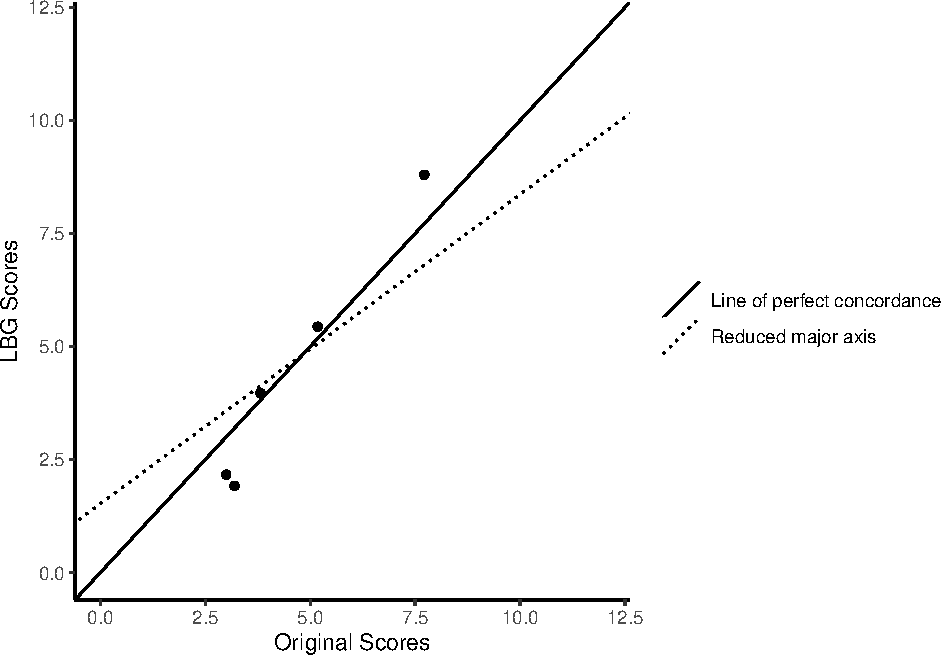
\includegraphics{_main_files/figure-latex/ggplot-wordscores-ccc-1.pdf}

This graph allows us to spot the problem. That is that while we gave the manifesto for Plaid Cymru (PCy) a reference score of 3.20, Wordscores gave it 1.91. Removing this manifesto from our data-set would thus improve our estimates.

Apart from positioning the texts, we can also have a look at the words themselves. We can do this with the \texttt{textplot\_scale1d} command, for which we also specify some words to highlight:

\begin{Shaded}
\begin{Highlighting}[]
\FunctionTok{library}\NormalTok{(quanteda.textplots)}

\FunctionTok{textplot\_scale1d}\NormalTok{(ws, }
                 \AttributeTok{margin =} \StringTok{"features"}\NormalTok{, }
                 \AttributeTok{highlighted =}\FunctionTok{c}\NormalTok{(}\StringTok{"british"}\NormalTok{,}\StringTok{"vote"}\NormalTok{, }\StringTok{"europe"}\NormalTok{, }\StringTok{"taxes"}\NormalTok{)}
\NormalTok{                 )}
\end{Highlighting}
\end{Shaded}

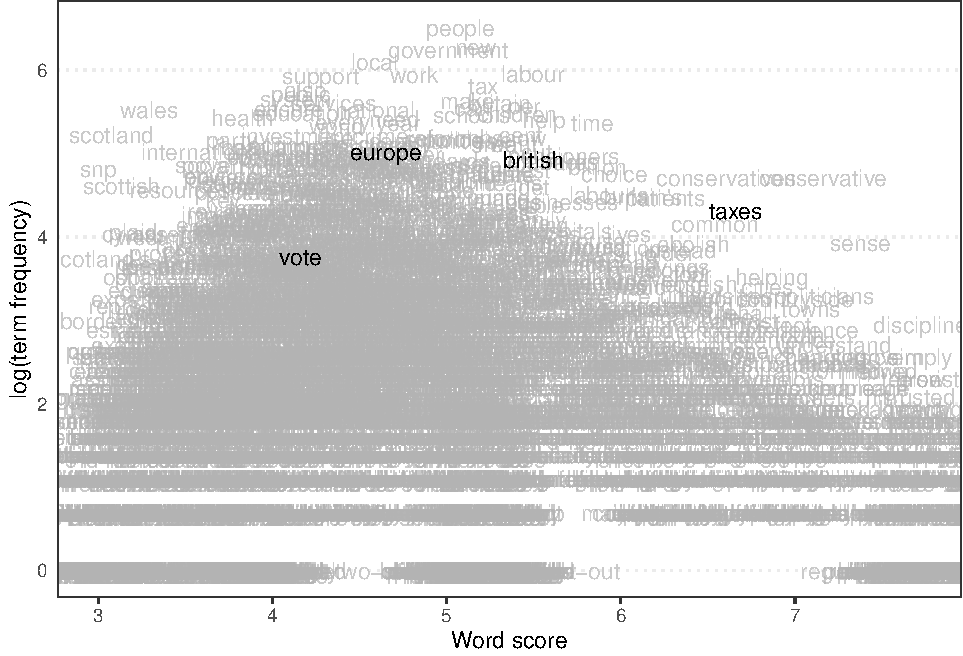
\includegraphics{_main_files/figure-latex/wordscores-textplotscale-features-1.pdf}

Finally, we can have a look at the confidence intervals around the scores we created. For this, we use the same command as above, though instead of specifying \texttt{features} (referring to the words), we specify \texttt{texts}. Note that we can only do this for the MV scores, as only here we also calculated the standard errors:

\begin{Shaded}
\begin{Highlighting}[]
\FunctionTok{textplot\_scale1d}\NormalTok{(pred\_mv, }\AttributeTok{margin =} \StringTok{"documents"}\NormalTok{)}
\end{Highlighting}
\end{Shaded}

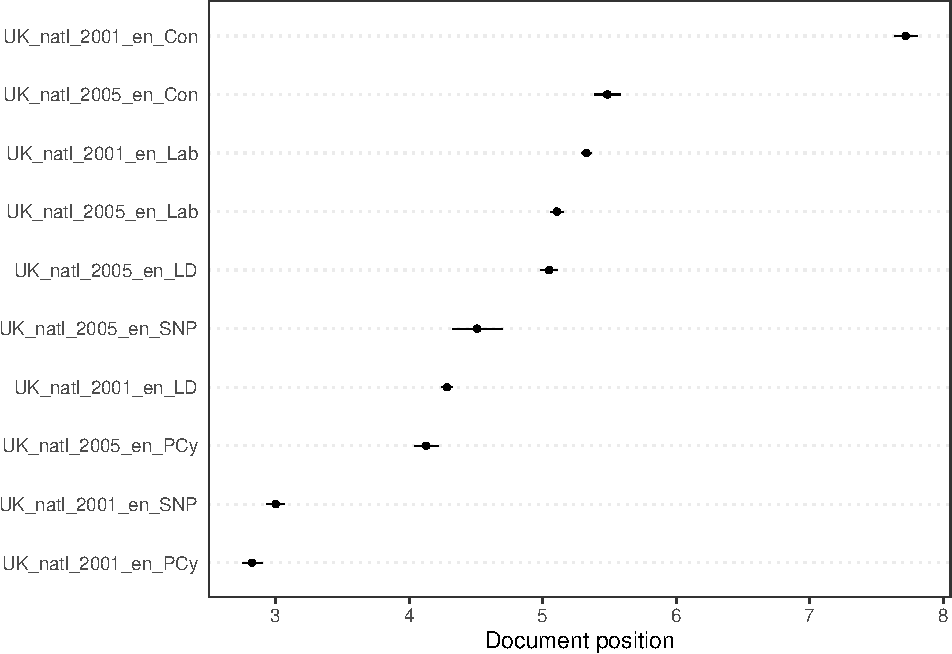
\includegraphics{_main_files/figure-latex/wordscores-textplotscale-documents-1.pdf}

Note that we can also make this graph ourselves. This requires some data-wrangling using the \texttt{dplyr} package. This package allows us to use pipes, denoted by the \texttt{\%\textgreater{}\%} command. This pipe transports an output of a command to another one before saving it. This saves us from constructing too many intermediate data sets. Thus, here we first bind together the row names of the fit (which denotes the documents), the fit itself, and the standard error of the fit (which also includes the lower and upper bound). We then transform this into a tibble (similar to a data frame), rename the first and fifth columns, and finally ensure that all the values (which are still characters) are numeric (and year a factor):

\begin{Shaded}
\begin{Highlighting}[]
\FunctionTok{library}\NormalTok{(dplyr)}

\NormalTok{data\_textplot }\OtherTok{\textless{}{-}} \FunctionTok{cbind}\NormalTok{(}\FunctionTok{rownames}\NormalTok{(}\FunctionTok{as.data.frame}\NormalTok{(pred\_mv}\SpecialCharTok{$}\NormalTok{se.fit)), pred\_mv}\SpecialCharTok{$}\NormalTok{fit, pred\_mv}\SpecialCharTok{$}\NormalTok{se.fit) }\SpecialCharTok{\%\textgreater{}\%}
 \FunctionTok{as\_tibble}\NormalTok{() }\SpecialCharTok{\%\textgreater{}\%}
 \FunctionTok{rename}\NormalTok{(}\AttributeTok{id =} \DecValTok{1}\NormalTok{, }\AttributeTok{se =} \DecValTok{5}\NormalTok{) }\SpecialCharTok{\%\textgreater{}\%}
 \FunctionTok{mutate}\NormalTok{(}\AttributeTok{fit =} \FunctionTok{as.numeric}\NormalTok{(fit),}
        \AttributeTok{lwr =} \FunctionTok{as.numeric}\NormalTok{(lwr),}
        \AttributeTok{upr =} \FunctionTok{as.numeric}\NormalTok{(upr),}
        \AttributeTok{se =} \FunctionTok{as.numeric}\NormalTok{(se),}
        \AttributeTok{year =} \FunctionTok{as.factor}\NormalTok{(stringr}\SpecialCharTok{::}\FunctionTok{str\_sub}\NormalTok{(id, }\AttributeTok{start =} \DecValTok{9}\NormalTok{, }\AttributeTok{end =} \DecValTok{12}\NormalTok{)))}
\end{Highlighting}
\end{Shaded}

If we now look at our \texttt{data\_textplot} object, we see that we have all the data we need: the fit (the average value), the lower and upper bounds, the year and the id that tells us with which party and year we are dealing. The only thing that remains is to give the parties better names. To see the current ones, type \texttt{data\_textplot\$id} in the console. We can then give them different names (ensure that the order remains the same). We then sort them in decreasing order based on their fit:

\begin{Shaded}
\begin{Highlighting}[]
\NormalTok{data\_textplot}\SpecialCharTok{$}\NormalTok{id }\OtherTok{\textless{}{-}} \FunctionTok{as.character}\NormalTok{(}\FunctionTok{c}\NormalTok{(}\StringTok{"CON 2001"}\NormalTok{, }\StringTok{"LAB 2001"}\NormalTok{, }\StringTok{"LD 2001"}\NormalTok{, }\StringTok{"PCY 2001"}\NormalTok{, }\StringTok{"SNP 2001"}\NormalTok{, }\StringTok{"CON 2005"}\NormalTok{,}\StringTok{"LAB 2005"}\NormalTok{, }\StringTok{"LD 2005"}\NormalTok{,}\StringTok{"PCY 2005"}\NormalTok{, }\StringTok{"SNP 2005"}\NormalTok{))}
\NormalTok{data\_textplot}\SpecialCharTok{$}\NormalTok{id }\OtherTok{\textless{}{-}} \FunctionTok{with}\NormalTok{(data\_textplot, }\FunctionTok{reorder}\NormalTok{(id, fit))}
\end{Highlighting}
\end{Shaded}

Then, we can plot this data using \texttt{ggplot}:

\begin{Shaded}
\begin{Highlighting}[]
\FunctionTok{ggplot}\NormalTok{() }\SpecialCharTok{+}
 \FunctionTok{geom\_point}\NormalTok{(}\AttributeTok{data =}\NormalTok{ data\_textplot,}
            \FunctionTok{aes}\NormalTok{(}\AttributeTok{x =}\NormalTok{ fit, }\AttributeTok{y =}\NormalTok{ id, }\AttributeTok{colour =}\NormalTok{ year)) }\SpecialCharTok{+}
 \FunctionTok{geom\_errorbarh}\NormalTok{(}\AttributeTok{data =}\NormalTok{ data\_textplot,}
                \FunctionTok{aes}\NormalTok{(}\AttributeTok{xmax =}\NormalTok{ upr, }\AttributeTok{xmin =}\NormalTok{ lwr, }\AttributeTok{y =}\NormalTok{ id, }\AttributeTok{colour =}\NormalTok{ year),}
                \AttributeTok{height =} \DecValTok{0}\NormalTok{) }\SpecialCharTok{+}
 \FunctionTok{theme\_classic}\NormalTok{() }\SpecialCharTok{+}
 \FunctionTok{scale\_colour\_manual}\NormalTok{(}\AttributeTok{values =} \FunctionTok{c}\NormalTok{(}\StringTok{"\#ffa600"}\NormalTok{, }\StringTok{"\#ff6361"}\NormalTok{),}
                     \AttributeTok{name =} \StringTok{"Years:"}\NormalTok{,}
                     \AttributeTok{breaks =} \FunctionTok{c}\NormalTok{(}\StringTok{"2001"}\NormalTok{, }\StringTok{"2005"}\NormalTok{),}
                     \AttributeTok{labels =} \FunctionTok{c}\NormalTok{(}\StringTok{"2001"}\NormalTok{, }\StringTok{"2005"}\NormalTok{)) }\SpecialCharTok{+}
 \FunctionTok{labs}\NormalTok{(}\AttributeTok{title =} \StringTok{"Left{-}Right Distribution of UK Party Manifestos"}\NormalTok{,}
      \AttributeTok{subtitle =} \StringTok{"with 95\% confidence intervals"}\NormalTok{,}
      \AttributeTok{x =} \StringTok{"Left {-} Right Score"}\NormalTok{,}
      \AttributeTok{y =} \ConstantTok{NULL}\NormalTok{) }\SpecialCharTok{+}
 \FunctionTok{theme\_classic}\NormalTok{()}\SpecialCharTok{+}
 \FunctionTok{theme}\NormalTok{(}\AttributeTok{plot.title =} \FunctionTok{element\_text}\NormalTok{(}\AttributeTok{size =} \DecValTok{20}\NormalTok{, }\AttributeTok{hjust =} \FloatTok{0.5}\NormalTok{),}
       \AttributeTok{plot.subtitle =} \FunctionTok{element\_text}\NormalTok{(}\AttributeTok{hjust =} \FloatTok{0.5}\NormalTok{),}
       \AttributeTok{legend.position =} \StringTok{"top"}\NormalTok{)}
\end{Highlighting}
\end{Shaded}

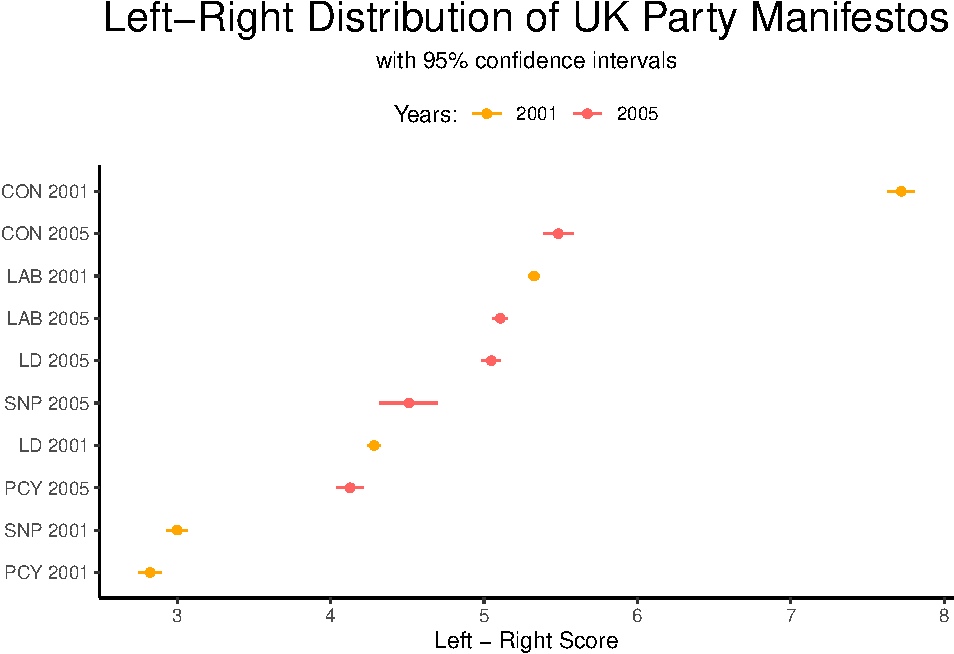
\includegraphics{_main_files/figure-latex/ggplot-wordscores-textplotscale-1.pdf}

\section{Wordfish}\label{wordfish}

Different from Wordscores, for Wordfish we do not need any reference text. Instead of this, the method using a model (based on a Poisson distribution) to calculate the scores for the texts. The only thing we have to tell Wordfish is which texts define the extremes of our scale. While this might seems very practical, it also leaves us with a problem: which scale do we want? For example, let us have another look at the corpus of inaugural speeches of American presidents we saw earlier. What scale should we expect? Let us, for now, say that we care about a general left-right position. As benchmarks, we then set the 1965 Johnson speech as the most ``left'' and the 1985 Reagan speech as the most ``right''. Also, we set a seed as the model draws random numbers and we want our work to be replicable:

\begin{Shaded}
\begin{Highlighting}[]
\FunctionTok{set.seed}\NormalTok{(}\DecValTok{42}\NormalTok{)}

\FunctionTok{library}\NormalTok{(quanteda)}

\FunctionTok{data}\NormalTok{(data\_corpus\_inaugural)}
\NormalTok{corpus\_inaugural }\OtherTok{\textless{}{-}} \FunctionTok{corpus\_subset}\NormalTok{(data\_corpus\_inaugural, Year }\SpecialCharTok{\textgreater{}} \DecValTok{1900}\NormalTok{)}

\NormalTok{data\_inaugural\_tokens }\OtherTok{\textless{}{-}} \FunctionTok{tokens}\NormalTok{(}
\NormalTok{ corpus\_inaugural,}
 \AttributeTok{what =} \StringTok{"word"}\NormalTok{,}
 \AttributeTok{remove\_punct =} \ConstantTok{TRUE}\NormalTok{,}
 \AttributeTok{remove\_symbols =} \ConstantTok{TRUE}\NormalTok{,}
 \AttributeTok{remove\_numbers =} \ConstantTok{TRUE}\NormalTok{,}
 \AttributeTok{remove\_url =} \ConstantTok{TRUE}\NormalTok{,}
 \AttributeTok{remove\_separators =} \ConstantTok{TRUE}\NormalTok{,}
 \AttributeTok{split\_hyphens =} \ConstantTok{FALSE}\NormalTok{,}
 \AttributeTok{include\_docvars =} \ConstantTok{TRUE}\NormalTok{,}
 \AttributeTok{padding =} \ConstantTok{FALSE}\NormalTok{,}
 \AttributeTok{verbose =} \ConstantTok{TRUE}
\NormalTok{)}

\NormalTok{data\_inaugural\_tokens }\OtherTok{\textless{}{-}} \FunctionTok{tokens\_tolower}\NormalTok{(data\_inaugural\_tokens, }\AttributeTok{keep\_acronyms =} \ConstantTok{FALSE}\NormalTok{)}
\NormalTok{data\_inaugural\_tokens }\OtherTok{\textless{}{-}} \FunctionTok{tokens\_select}\NormalTok{(data\_inaugural\_tokens, }\FunctionTok{stopwords}\NormalTok{(}\StringTok{"english"}\NormalTok{), }\AttributeTok{selection =} \StringTok{"remove"}\NormalTok{)}

\NormalTok{data\_inaugural\_dfm }\OtherTok{\textless{}{-}} \FunctionTok{dfm}\NormalTok{(data\_inaugural\_tokens)}

\NormalTok{data\_inaugural\_dfm}\SpecialCharTok{@}\NormalTok{Dimnames}\SpecialCharTok{$}\NormalTok{docs}
\NormalTok{wordfish }\OtherTok{\textless{}{-}} \FunctionTok{textmodel\_wordfish}\NormalTok{(data\_inaugural\_dfm, }\AttributeTok{dir =} \FunctionTok{c}\NormalTok{(}\DecValTok{17}\NormalTok{,}\DecValTok{22}\NormalTok{))}
\FunctionTok{summary}\NormalTok{(wordfish)}
\end{Highlighting}
\end{Shaded}

Here, \texttt{theta} gives us the position of the text. As with Wordscores, we can also calculate the confidence intervals (note that \texttt{theta} is now called \texttt{fit}):

\begin{Shaded}
\begin{Highlighting}[]
\NormalTok{pred\_wordfish }\OtherTok{\textless{}{-}} \FunctionTok{predict}\NormalTok{(wordfish, }\AttributeTok{interval =} \StringTok{"confidence"}\NormalTok{)}
\FunctionTok{head}\NormalTok{(pred\_wordfish)}
\end{Highlighting}
\end{Shaded}

\begin{verbatim}
## $fit
##                        fit         lwr         upr
## 1901-McKinley    1.5264409  1.45790457  1.59497725
## 1905-Roosevelt   0.5506952  0.40261155  0.69877876
## 1909-Taft        2.1180136  2.08705631  2.14897090
## 1913-Wilson      0.9494614  0.84832377  1.05059905
## 1917-Wilson      0.8648796  0.75150283  0.97825636
## 1921-Harding     1.3071861  1.24655829  1.36781392
## 1925-Coolidge    1.4398978  1.38585947  1.49393615
## 1929-Hoover      1.5400830  1.48640261  1.59376344
## 1933-Roosevelt   1.1206324  1.03168956  1.20957530
## 1937-Roosevelt   0.6493799  0.54742236  0.75133754
## 1941-Roosevelt   0.1153382 -0.01421607  0.24489242
## 1945-Roosevelt  -0.1670750 -0.36383112  0.02968117
## 1949-Truman      0.8432860  0.75602390  0.93054816
## 1953-Eisenhower  0.2792466  0.18725486  0.37123825
## 1957-Eisenhower  0.1574969  0.04465718  0.27033658
## 1961-Kennedy    -0.5395875 -0.64994887 -0.42922607
## 1965-Johnson    -0.7821091 -0.88376502 -0.68045324
## 1969-Nixon      -0.9602454 -1.03699050 -0.88350021
## 1973-Nixon      -0.4420077 -0.54461368 -0.33940174
## 1977-Carter     -0.3423320 -0.46809663 -0.21656746
## 1981-Reagan     -0.6953845 -0.77712614 -0.61364280
## 1985-Reagan     -0.6413867 -0.71992268 -0.56285068
## 1989-Bush       -0.8785297 -0.95604292 -0.80101647
## 1993-Clinton    -1.1462836 -1.22477539 -1.06779189
## 1997-Clinton    -0.8669737 -0.94358633 -0.79036108
## 2001-Bush       -0.7438888 -0.84090471 -0.64687286
## 2005-Bush       -0.4113008 -0.50479109 -0.31781044
## 2009-Obama      -1.0807899 -1.14809049 -1.01348932
## 2013-Obama      -1.0547830 -1.12762813 -0.98193782
## 2017-Trump      -1.3804172 -1.45178196 -1.30905236
## 2021-Biden      -1.3289432 -1.38772817 -1.27015814
\end{verbatim}

As with Wordscores, we can also plot graphs for Wordfish, using the same commands. The first graph we will again be looking at is the distribution of the words, which here forms an `Eifel Tower'-like graph:

\begin{Shaded}
\begin{Highlighting}[]
\FunctionTok{textplot\_scale1d}\NormalTok{(wordfish,}
                 \AttributeTok{margin =} \StringTok{"features"}\NormalTok{,}
                 \AttributeTok{highlighted =} \FunctionTok{c}\NormalTok{(}\StringTok{"america"}\NormalTok{,}\StringTok{"jobs"}\NormalTok{,}\StringTok{"taxes"}\NormalTok{,}\StringTok{"election"}\NormalTok{)}
\NormalTok{                 )}
\end{Highlighting}
\end{Shaded}

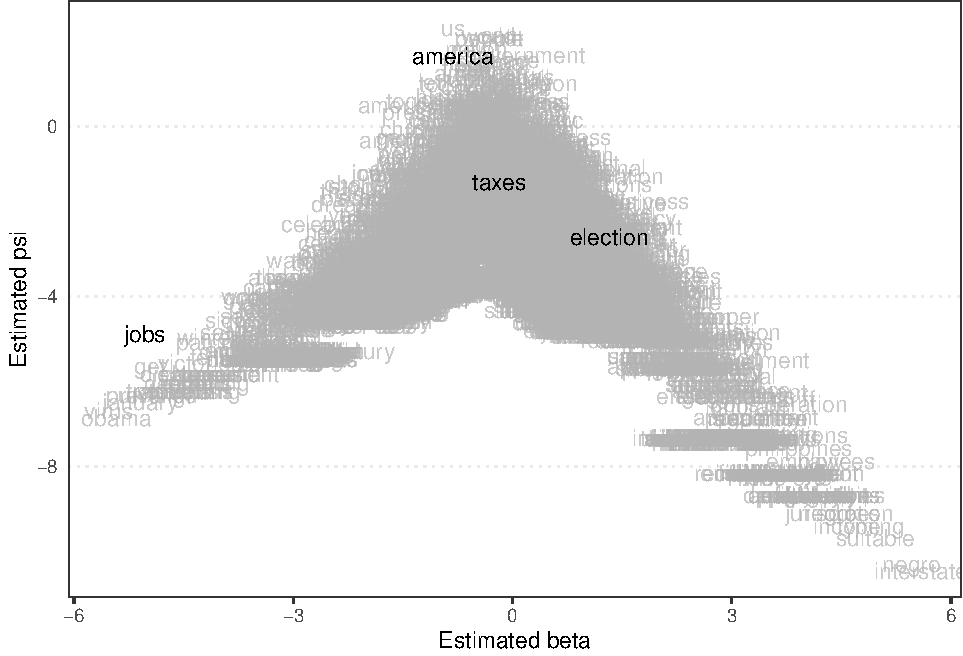
\includegraphics{_main_files/figure-latex/wordfish-textplot-features-1.pdf}

And then we can do the same for the documents as well. Note that we can also make a similar graph to the one we made ourselves above (just replace \texttt{pred\_mv} with \texttt{pred\_wordfish}):

\begin{Shaded}
\begin{Highlighting}[]
\FunctionTok{textplot\_scale1d}\NormalTok{(wordfish,}
                 \AttributeTok{margin =} \StringTok{"documents"}
\NormalTok{                 )}
\end{Highlighting}
\end{Shaded}

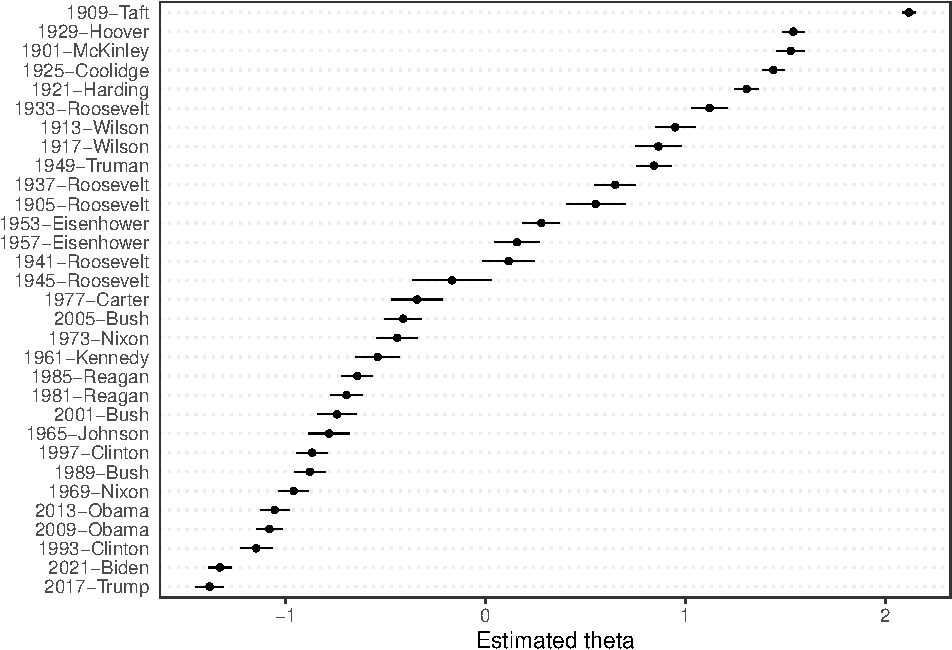
\includegraphics{_main_files/figure-latex/wordfish-textplot-documents-1.pdf}

Looking at the results here gives us an interesting picture. Remember that we chose our benchmark texts to look at the left-right position of our texts? Here, we see that both these texts (the 1965 Johnson and 1985 Reagan) are quite close to each other. Sticking with our interpretation that Reagan is more right-wing than Johnson, this would mean that the 1909 Taft address was the most right-wing and the 2017 Trump text the most left-wing. Whether this is true is of course up to our interpretation.

\section{Correspondence Analysis}\label{correspondence-analysis}

Correspondence Analysis uses a similar logic as Principal Component Analysis. Yet, while PCA requires metric data, CA only requires nominal data (such as text). The idea behind both is to reduce the complexity of the data by looking for new dimensions. These dimensions should then explain as much of the original variance that is present in the data as possible. Within R many packages can run CA (such as the \texttt{ca} and \texttt{FactoMineR} packages and even \texttt{quanteda.textmodels}). One interesting package is the \texttt{R.temis} package. This package aims to bring the techniques of qualitative text analysis into R. Thus, the package focuses on the import of corpus from programs such as \href{https://www.image-zafar.com/Logicieluk.html}{Alceste} and sites such as \href{https://www.lexisnexis.com}{LexisNexis} - programs that are often used in qualitative text analysis. The package itself is built on the popular \texttt{tm} package and has a similar logic.

To carry out the Correspondence Analysis, \texttt{R.temis} uses the \texttt{FactoMineR} and \texttt{factoextra} packages (\citeproc{ref-Le2008a}{Lê et al., 2008}). Here, we will look at an example using data from an article on the stylistic variations in the Twitter data of Donald Trump between 2009 and 2018 (\citeproc{ref-Clarke2019a}{Clarke \& Grieve, 2019}). Here, the authors aimed to figure out whether the way Trump's tweets were written fluctuated over time. To do so, they downloaded 21,739 tweets and grouped them into 63 categories over 4 dimensions based on their content. Given that all the data used in the article is available for inspection, we can attempt to replicate part of the analysis here.

First, we load the packages we need for the Correspondence Analysis:

\begin{Shaded}
\begin{Highlighting}[]
\FunctionTok{library}\NormalTok{(FactoMineR)}
\FunctionTok{library}\NormalTok{(factoextra)}
\FunctionTok{library}\NormalTok{(readr)}
\end{Highlighting}
\end{Shaded}

Then, we import the data. You can do so either by downloading the replication data yourselves, or use the file we already put up on GitHub:

\begin{Shaded}
\begin{Highlighting}[]
\NormalTok{urlfile }\OtherTok{=} \StringTok{"https://raw.githubusercontent.com/SCJBruinsma/qta{-}files/master/TRUMP\_DATA.csv"}
\NormalTok{tweets }\OtherTok{\textless{}{-}} \FunctionTok{read\_csv}\NormalTok{(}\FunctionTok{url}\NormalTok{(urlfile), }\AttributeTok{show\_col\_types =} \ConstantTok{FALSE}\NormalTok{)}
\end{Highlighting}
\end{Shaded}

This data set contains quite some information we do not need. To begin with, we remove all those variables that do not contain information about the 63 categories and the length of the tweet in words. Also, for clarity's sake, we sample 200 of the tweets:

\begin{Shaded}
\begin{Highlighting}[]
\NormalTok{tweets }\OtherTok{\textless{}{-}}\NormalTok{ tweets[}\FunctionTok{sample}\NormalTok{(}\FunctionTok{nrow}\NormalTok{(tweets), }\DecValTok{200}\NormalTok{), ]}
\NormalTok{tweets\_mat }\OtherTok{\textless{}{-}}\NormalTok{ tweets[,}\DecValTok{2}\SpecialCharTok{:}\DecValTok{65}\NormalTok{]}
\end{Highlighting}
\end{Shaded}

We can then run the MCA with the \texttt{FactoMineR} package. For this, we have to give the data set and the number of dimensions we think are in the data. We can set the latter either by establishing the dimensions as in a regular PCA (for example through a scree plot) or based on theory. Here we combine both and use the 5 dimensions established in the article. Besides this, we set a supplementary quantitative variable as \texttt{quanti.sup=1}. As this is a quantitative variable, it is not taken into consideration by the MCA, but does allow us to assess later on how it correlates with each of the five dimensions:

\begin{Shaded}
\begin{Highlighting}[]
\NormalTok{mca\_tweets }\OtherTok{\textless{}{-}} \FunctionTok{MCA}\NormalTok{(tweets\_mat, }\AttributeTok{ncp=}\DecValTok{5}\NormalTok{, }\AttributeTok{quanti.sup=}\DecValTok{1}\NormalTok{, }\AttributeTok{graph =} \ConstantTok{FALSE}\NormalTok{)}
\end{Highlighting}
\end{Shaded}

First, let's start by looking at the association of the word length with the five dimensions:

\begin{Shaded}
\begin{Highlighting}[]
\NormalTok{mca\_tweets}\SpecialCharTok{$}\NormalTok{quanti.sup}
\end{Highlighting}
\end{Shaded}

\begin{verbatim}
## $coord
##               Dim 1      Dim 2      Dim 3      Dim 4       Dim 5
## WORDCOUNT 0.8668104 -0.2107786 0.02090331 0.03345767 -0.05383935
\end{verbatim}

As we can see, the word length has a strong correlation with Dimension 1. This means that this dimension captures the length of the words and is not a separate dimension. Thus, when we want to look at the correspondence between the categories and the dimensions, we can ignore this dimension. Thus, for the MCA, we will look at dimensions 2 and 3:

\begin{Shaded}
\begin{Highlighting}[]
\FunctionTok{fviz\_mca\_var}\NormalTok{(mca\_tweets,}
             \AttributeTok{repel =} \ConstantTok{TRUE}\NormalTok{,}
             \AttributeTok{geom =} \FunctionTok{c}\NormalTok{(}\StringTok{"point"}\NormalTok{),}
             \AttributeTok{axes =} \FunctionTok{c}\NormalTok{(}\DecValTok{2}\NormalTok{, }\DecValTok{3}\NormalTok{),}
             \AttributeTok{ggtheme =} \FunctionTok{theme\_minimal}\NormalTok{()}
\NormalTok{             )}
\end{Highlighting}
\end{Shaded}

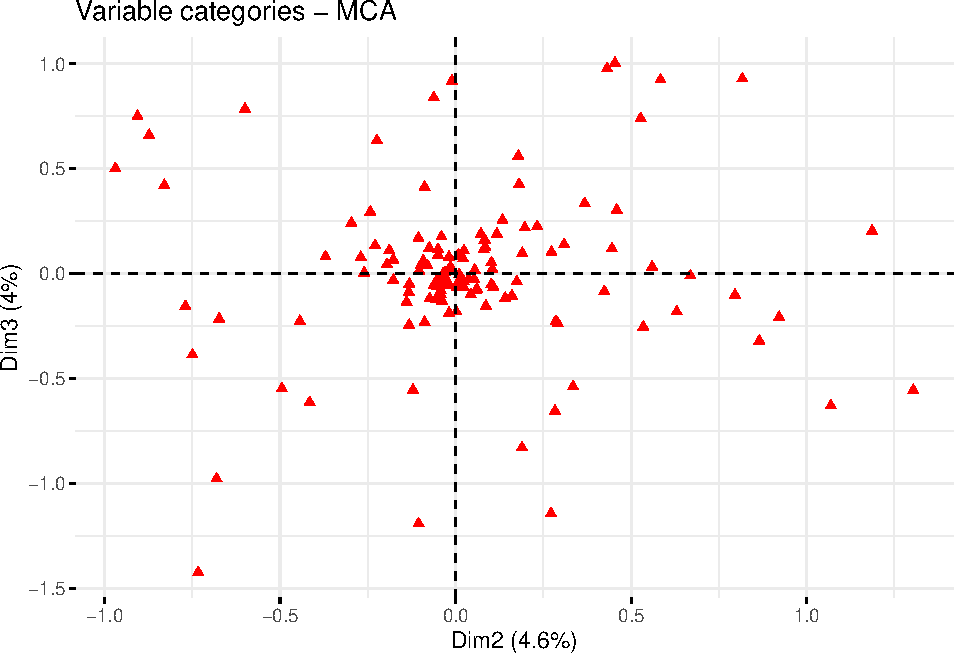
\includegraphics{_main_files/figure-latex/trumptweets-fvizvar-1.pdf}

Here, we only plot the points as adding the labels as well will make the picture quite cluttered. In the article, the authors identify Dimension 2 as `Conversational Style' and Dimension 3 as `Campaigning Style'. The plot thus shows us that some categories belong to one of these dimensions and not to the other. To see for which cases this is most often the case (the ones that have the most extreme positions), we can have a look at their coordinates:

\begin{Shaded}
\begin{Highlighting}[]
\NormalTok{var }\OtherTok{\textless{}{-}} \FunctionTok{get\_mca\_var}\NormalTok{(mca\_tweets)}
\NormalTok{coordinates }\OtherTok{\textless{}{-}} \FunctionTok{as.data.frame}\NormalTok{(var}\SpecialCharTok{$}\NormalTok{coord)}
\NormalTok{coordinates }\OtherTok{\textless{}{-}}\NormalTok{ coordinates[}\FunctionTok{order}\NormalTok{(coordinates}\SpecialCharTok{$}\StringTok{\textasciigrave{}}\AttributeTok{Dim 2}\StringTok{\textasciigrave{}}\NormalTok{),]}
\FunctionTok{head}\NormalTok{(coordinates)}
\end{Highlighting}
\end{Shaded}

\begin{verbatim}
##                     Dim 1      Dim 2      Dim 3        Dim 4       Dim 5
## POSESPRPN_P    0.03383985 -0.9689511  0.5011988  0.036488377  0.36083073
## PROGRESSIVE_P  0.79201463 -0.9059134  0.7499092 -0.674316668  0.46134193
## SUPERLATIVE_P  0.37755724 -0.8728057  0.6594311 -0.147514294 -0.41714831
## GERUND_P       0.20213101 -0.8295159  0.4209137  0.089642937  0.82377111
## MULTIWVB_P     0.42162442 -0.7694130 -0.1558600 -0.003865414  0.37457619
## COLON_P       -0.24915096 -0.7493897 -0.3866968  1.023830211 -0.07073923
\end{verbatim}

Here, remember to look only at the results from the second column onward. Here, we see that one extreme category for the second dimension (Conversational Style) was the use of a colon (:) or possessive proper nouns (such as Hillary's). This seems to fit well with the idea of conversational style. We can also see that the latter one also corresponds quite well with Dimension 3 (Campaigning Style), while the first one does not.

As you can see, the possibilities with MCA call for a rather investigative approach. For this reason, the designers of \texttt{FactoMineR} developed a Shiny app that allows you to play around with the data and look at all the various options. Load it by running:

\begin{Shaded}
\begin{Highlighting}[]
\FunctionTok{library}\NormalTok{(Factoshiny)}
\NormalTok{res.shiny }\OtherTok{\textless{}{-}} \FunctionTok{MCAshiny}\NormalTok{(tweets\_mat)}
\end{Highlighting}
\end{Shaded}

Ensure you quit by clicking the ``Quit the App'' button to return to R. For more information on the `Facto'-family packages, please have a look at the original article by Lê et al. (\citeproc{ref-Le2008a}{2008}) or the website that belongs to it: \url{http://factominer.free.fr/}.

\chapter{Supervised Methods}\label{supervised-methods}

While with scaling we try to place our texts on a scale, with supervised methods we go back to what we did with dictionary analysis: classification. Within \texttt{quanteda} there are many different models for supervised methods, of which we will cover two. These are \emph{Support Vector Machines} (SVM) and \emph{Naive Bayes} (NB). The first classifies texts by looking at their position on a hyperplane, the second by their (Bayesian) probabilities.

\section{Support Vector Machines}\label{support-vector-machines}

To show how SVM works, we will look at an example of SVM in \texttt{quanteda} and one in \texttt{RTextTools}, and an example of NB in \texttt{quanteda}.

\subsection{SVM with RTextTools}\label{svm-with-rtexttools}

For the SVM, we will start with an example using our Twitter data and the \texttt{RTextTools} package. First, we load the Twitter data:

\begin{Shaded}
\begin{Highlighting}[]
\FunctionTok{library}\NormalTok{(}\StringTok{"RTextTools"}\NormalTok{)}
\FunctionTok{library}\NormalTok{(}\StringTok{"car"}\NormalTok{)}

\NormalTok{urlfile }\OtherTok{\textless{}{-}} \StringTok{"https://raw.githubusercontent.com/SCJBruinsma/qta{-}files/master/Tweets.csv"}
\NormalTok{tweets }\OtherTok{\textless{}{-}} \FunctionTok{read.csv}\NormalTok{(}\FunctionTok{url}\NormalTok{(urlfile))}
\NormalTok{tweets}\SpecialCharTok{$}\NormalTok{text }\OtherTok{\textless{}{-}} \FunctionTok{gsub}\NormalTok{(}\StringTok{"http.*"}\NormalTok{,}\StringTok{""}\NormalTok{, tweets}\SpecialCharTok{$}\NormalTok{text)}
\NormalTok{tweets}\SpecialCharTok{$}\NormalTok{text }\OtherTok{\textless{}{-}} \FunctionTok{gsub}\NormalTok{(}\StringTok{"https.*"}\NormalTok{,}\StringTok{""}\NormalTok{, tweets}\SpecialCharTok{$}\NormalTok{text)}
\NormalTok{tweets}\SpecialCharTok{$}\NormalTok{text }\OtherTok{\textless{}{-}} \FunctionTok{gsub}\NormalTok{(}\StringTok{"}\SpecialCharTok{\textbackslash{}\textbackslash{}}\StringTok{$"}\NormalTok{, }\StringTok{""}\NormalTok{, tweets}\SpecialCharTok{$}\NormalTok{text) }
\NormalTok{tweets}\SpecialCharTok{$}\NormalTok{text }\OtherTok{\textless{}{-}} \FunctionTok{gsub}\NormalTok{(}\StringTok{"@}\SpecialCharTok{\textbackslash{}\textbackslash{}}\StringTok{w+"}\NormalTok{, }\StringTok{""}\NormalTok{, tweets}\SpecialCharTok{$}\NormalTok{text) }
\NormalTok{tweets}\SpecialCharTok{$}\NormalTok{text }\OtherTok{\textless{}{-}} \FunctionTok{gsub}\NormalTok{(}\StringTok{"[[:punct:]]"}\NormalTok{, }\StringTok{""}\NormalTok{, tweets}\SpecialCharTok{$}\NormalTok{text) }
\NormalTok{tweets}\SpecialCharTok{$}\NormalTok{text }\OtherTok{\textless{}{-}} \FunctionTok{gsub}\NormalTok{(}\StringTok{"[ |}\SpecialCharTok{\textbackslash{}t}\StringTok{]\{2,\}"}\NormalTok{, }\StringTok{""}\NormalTok{, tweets}\SpecialCharTok{$}\NormalTok{text) }
\NormalTok{tweets}\SpecialCharTok{$}\NormalTok{text }\OtherTok{\textless{}{-}} \FunctionTok{gsub}\NormalTok{(}\StringTok{"\^{} "}\NormalTok{, }\StringTok{""}\NormalTok{, tweets}\SpecialCharTok{$}\NormalTok{text) }
\NormalTok{tweets}\SpecialCharTok{$}\NormalTok{text }\OtherTok{\textless{}{-}} \FunctionTok{gsub}\NormalTok{(}\StringTok{" $"}\NormalTok{, }\StringTok{""}\NormalTok{, tweets}\SpecialCharTok{$}\NormalTok{text) }
\NormalTok{tweets}\SpecialCharTok{$}\NormalTok{text }\OtherTok{\textless{}{-}} \FunctionTok{gsub}\NormalTok{(}\StringTok{"RT"}\NormalTok{, }\StringTok{""}\NormalTok{, tweets}\SpecialCharTok{$}\NormalTok{text) }
\NormalTok{tweets}\SpecialCharTok{$}\NormalTok{text }\OtherTok{\textless{}{-}} \FunctionTok{gsub}\NormalTok{(}\StringTok{"href"}\NormalTok{, }\StringTok{""}\NormalTok{, tweets}\SpecialCharTok{$}\NormalTok{text)}

\NormalTok{labels }\OtherTok{\textless{}{-}}\NormalTok{ tweets}\SpecialCharTok{$}\NormalTok{airline\_sentiment}
\NormalTok{labels }\OtherTok{\textless{}{-}}\NormalTok{ car}\SpecialCharTok{::}\FunctionTok{recode}\NormalTok{(labels, }\StringTok{"\textquotesingle{}positive\textquotesingle{}=1;\textquotesingle{}negative\textquotesingle{}={-}1;\textquotesingle{}neutral\textquotesingle{}=0"}\NormalTok{)}
\end{Highlighting}
\end{Shaded}

The goal of the supervised learning task is to use part of this dataset to train a certain algorithm and then use the trained algorithm to assign categories to the remaining sentences. Since we know the coded categories for the remaining sentences, we will be able to evaluate how well this training was in guessing/estimating what the codes for these sentences were. We start by creating a document term matrix;

\begin{Shaded}
\begin{Highlighting}[]
\NormalTok{doc\_matrix }\OtherTok{\textless{}{-}} \FunctionTok{create\_matrix}\NormalTok{(tweets}\SpecialCharTok{$}\NormalTok{text,}
                            \AttributeTok{language =} \StringTok{"english"}\NormalTok{, }
                            \AttributeTok{removeNumbers =} \ConstantTok{TRUE}\NormalTok{, }
                            \AttributeTok{stemWords =} \ConstantTok{TRUE}\NormalTok{, }
                            \AttributeTok{removeSparseTerms =} \FloatTok{0.998}\NormalTok{)}
\NormalTok{doc\_matrix}
\end{Highlighting}
\end{Shaded}

\begin{verbatim}
## <<DocumentTermMatrix (documents: 14640, terms: 693)>>
## Non-/sparse entries: 84521/10060999
## Sparsity           : 99%
## Maximal term length: 18
## Weighting          : term frequency (tf)
\end{verbatim}

Note that \texttt{RTextTools} gives you plenty of options in preprocessing. Apart from the options used above, we can also strip whitespace, remove punctuation, and remove stopwords. Stemming and stopword removal is language-specific, so when we select the language in the option above \texttt{(language=\textquotesingle{}\textquotesingle{}english\textquotesingle{}\textquotesingle{})}, \texttt{RTextTools} will carry this out according to our language of choice. As of now, the package supports Danish, Dutch, English, Finnish, French, German, Italian, Norwegian, Portuguese, Russian, Spanish, and Swedish.

We then create a container parsing the document matrix into a training set, and a test set. We will use the training set will to train the algorithm and the test set to test how well this algorithm was trained. The following command instructs R to use the first 4000 sentences for the training set the remaining 449 sentences for the test set. Moreover, we specify to append to the document matrix the variable that contains the assigned coders:

\begin{Shaded}
\begin{Highlighting}[]
\NormalTok{container }\OtherTok{\textless{}{-}} \FunctionTok{create\_container}\NormalTok{(doc\_matrix,}
\NormalTok{                              labels,}
                              \AttributeTok{trainSize =} \DecValTok{1}\SpecialCharTok{:}\DecValTok{10000}\NormalTok{, }
                              \AttributeTok{testSize =} \DecValTok{10001}\SpecialCharTok{:}\DecValTok{14640}\NormalTok{, }
                              \AttributeTok{virgin =} \ConstantTok{FALSE}\NormalTok{)}
\end{Highlighting}
\end{Shaded}

We can then train a model using one of the available algorithms. For instance, we can use the Support Vector Machines algorithm (SVM) as follows:

\begin{Shaded}
\begin{Highlighting}[]
\NormalTok{SVM }\OtherTok{\textless{}{-}} \FunctionTok{train\_model}\NormalTok{(container, }\StringTok{"SVM"}\NormalTok{)}
\end{Highlighting}
\end{Shaded}

Other algorithms are available if you change the SVM option. Options exist for Lasso and Elastic-Net Regularized Generalized Linear Models (\texttt{GLMNET}), maximum entropy (\texttt{MAXENT}), scaled linear discriminant analysis (\texttt{SLDA}), bagging (\texttt{BAGGING}), boosting (\texttt{BOOSTING}), random forests (\texttt{RF}), neural networks (\texttt{NNET}), or classification trees (\texttt{TREE}).

We then use the model we trained to classify the texts in the test set. The following command instructs R to classify the documents in the test set of the container using the SVM model that we trained earlier.

\begin{Shaded}
\begin{Highlighting}[]
\NormalTok{SVM\_CLASSIFY }\OtherTok{\textless{}{-}} \FunctionTok{classify\_model}\NormalTok{(container, SVM)}
\end{Highlighting}
\end{Shaded}

We can also view the classification that the SVM model performed as follows. The first column corresponds to the label that coders assigned to each of the tweets in the training set. The second column then gives the probability that the SVM algorithm assigned to that particular category. As you can see, while the probability for some sentences is quite high, for others it is quite low. This even while the classification always chooses the category with the highest probability.

\begin{Shaded}
\begin{Highlighting}[]
\FunctionTok{head}\NormalTok{(SVM\_CLASSIFY)}
\end{Highlighting}
\end{Shaded}

The next step is to check the classification performance of our model. To do this, we first request a function that returns a container with different summaries. For instance, we can request summaries based on the labels attached to the sentences, the documents (or in this case, the sentences) by label, or based on the algorithm.

\begin{Shaded}
\begin{Highlighting}[]
\NormalTok{analytics }\OtherTok{\textless{}{-}} \FunctionTok{create\_analytics}\NormalTok{(container, SVM\_CLASSIFY)}
\FunctionTok{summary}\NormalTok{(analytics)}
\end{Highlighting}
\end{Shaded}

\begin{verbatim}
## ENSEMBLE SUMMARY
## 
##        n-ENSEMBLE COVERAGE n-ENSEMBLE RECALL
## n >= 1                   1               0.8
## 
## 
## ALGORITHM PERFORMANCE
## 
## SVM_PRECISION    SVM_RECALL    SVM_FSCORE 
##     0.6833333     0.6766667     0.6800000
\end{verbatim}

Here, precision gives the proportion of bills that SVM classified as belonging to a category that does belong to that category (true positives) to all the bills that are classified in that category (irrespective of where they belong). Recall, then, is the proportion of bills that SVM classifies as belonging to a category and belong to this category (true positives) to all the bills that belong to this category (true positives plus false negatives). The F score is a weighted average between precision and recall ranging from 0 to 1.

Finally, we can compare the scores between the labels given by the coders and those based on our SVM:

\begin{Shaded}
\begin{Highlighting}[]
\NormalTok{compare }\OtherTok{\textless{}{-}} \FunctionTok{as.data.frame}\NormalTok{(}\FunctionTok{cbind}\NormalTok{(labels[}\DecValTok{10001}\SpecialCharTok{:}\DecValTok{14640}\NormalTok{], SVM\_CLASSIFY}\SpecialCharTok{$}\NormalTok{SVM\_LABEL))}
\FunctionTok{table}\NormalTok{(compare)}
\end{Highlighting}
\end{Shaded}

\begin{verbatim}
##     V2
## V1     -1    0    1
##   -1 3018  292  109
##   0   288  347   56
##   1   130   58  342
\end{verbatim}

\subsection{SVM with Quanteda}\label{svm-with-quanteda}

Instead of using a separate package, we can also use \texttt{quanteda} to carry out an SVM. For this, we load some movie reviews, select 1000 of them at random, and place them into our corpus:

\begin{Shaded}
\begin{Highlighting}[]
\FunctionTok{set.seed}\NormalTok{(}\DecValTok{42}\NormalTok{)}

\FunctionTok{library}\NormalTok{(quanteda)}
\FunctionTok{library}\NormalTok{(quanteda.classifiers)}
\NormalTok{corpus\_reviews }\OtherTok{\textless{}{-}} \FunctionTok{corpus\_sample}\NormalTok{(data\_corpus\_LMRD, }\DecValTok{1000}\NormalTok{)}
\end{Highlighting}
\end{Shaded}

Our aim here will be to see how well the SVM algorithm can predict the rating of the reviews. To do this, we first have to create a new variable \texttt{prediction}. This variable contains the same scores as the original rating. Then, we remove 30\% of the scores and replace them with NA. We do so by creating a \texttt{missing} variable that contains 30\% 0s and 70\% 1s. We then place the 0s with NAs. These NA scores are then the ones we want the algorithm to predict. Finally, we add the new variable to the corpus:

\begin{Shaded}
\begin{Highlighting}[]
\NormalTok{prediction }\OtherTok{\textless{}{-}}\NormalTok{ corpus\_reviews}\SpecialCharTok{$}\NormalTok{rating}

\NormalTok{missing }\OtherTok{\textless{}{-}} \FunctionTok{rbinom}\NormalTok{(}\DecValTok{1000}\NormalTok{, }\DecValTok{1}\NormalTok{, }\FloatTok{0.7}\NormalTok{)}
\NormalTok{prediction[missing }\SpecialCharTok{==} \DecValTok{0}\NormalTok{] }\OtherTok{\textless{}{-}} \ConstantTok{NA}

\FunctionTok{docvars}\NormalTok{(corpus\_reviews, }\StringTok{"prediction"}\NormalTok{) }\OtherTok{\textless{}{-}}\NormalTok{ prediction}
\end{Highlighting}
\end{Shaded}

We then transform the corpus into a data frame, and also remove stopwords, numbers and punctuation:

\begin{Shaded}
\begin{Highlighting}[]
\NormalTok{data\_reviews\_tokens }\OtherTok{\textless{}{-}} \FunctionTok{tokens}\NormalTok{(}
\NormalTok{ corpus\_reviews,}
 \AttributeTok{what =} \StringTok{"word"}\NormalTok{,}
 \AttributeTok{remove\_punct =} \ConstantTok{TRUE}\NormalTok{,}
 \AttributeTok{remove\_symbols =} \ConstantTok{TRUE}\NormalTok{,}
 \AttributeTok{remove\_numbers =} \ConstantTok{TRUE}\NormalTok{,}
 \AttributeTok{remove\_url =} \ConstantTok{TRUE}\NormalTok{,}
 \AttributeTok{remove\_separators =} \ConstantTok{TRUE}\NormalTok{,}
 \AttributeTok{split\_hyphens =} \ConstantTok{FALSE}\NormalTok{,}
 \AttributeTok{include\_docvars =} \ConstantTok{TRUE}\NormalTok{,}
 \AttributeTok{padding =} \ConstantTok{FALSE}\NormalTok{,}
 \AttributeTok{verbose =} \ConstantTok{TRUE}
\NormalTok{)}
\NormalTok{data\_reviews\_tokens }\OtherTok{\textless{}{-}} \FunctionTok{tokens\_tolower}\NormalTok{(data\_reviews\_tokens, }\AttributeTok{keep\_acronyms =} \ConstantTok{FALSE}\NormalTok{)}
\NormalTok{data\_reviews\_tokens }\OtherTok{\textless{}{-}} \FunctionTok{tokens\_select}\NormalTok{(data\_reviews\_tokens, }\FunctionTok{stopwords}\NormalTok{(}\StringTok{"english"}\NormalTok{), }\AttributeTok{selection =} \StringTok{"remove"}\NormalTok{)}
\NormalTok{dfm\_reviews }\OtherTok{\textless{}{-}} \FunctionTok{dfm}\NormalTok{(data\_reviews\_tokens)}
\end{Highlighting}
\end{Shaded}

Now we can run the SVM algorithm. To do so, we tell the model on which dfm we want to run our model, and which variable contains the scores to train the algorithm. Here, this is our \texttt{prediction} variable with the missing data:

\begin{Shaded}
\begin{Highlighting}[]
\FunctionTok{library}\NormalTok{(quanteda.textmodels)}
\NormalTok{svm\_reviews }\OtherTok{\textless{}{-}} \FunctionTok{textmodel\_svm}\NormalTok{(dfm\_reviews, }\AttributeTok{y =} \FunctionTok{docvars}\NormalTok{(dfm\_reviews, }\StringTok{"prediction"}\NormalTok{))}
\NormalTok{svm\_reviews}
\end{Highlighting}
\end{Shaded}

\begin{verbatim}
## 
## Call:
## textmodel_svm.dfm(x = dfm_reviews, y = docvars(dfm_reviews, "prediction"))
## 
## 672 training documents; 121,240 fitted features.
## Method: L2-regularized L2-loss support vector classification dual (L2R_L2LOSS_SVC_DUAL)
\end{verbatim}

Here we see that the algorithm used 672 texts to train the model (the one with a score) and fitted 133,728 features. The latter refers to the total number of words in the training texts and not only the unique ones. Now we can use this model to predict the ratings we removed earlier:

\begin{Shaded}
\begin{Highlighting}[]
\NormalTok{svm\_predict }\OtherTok{\textless{}{-}} \FunctionTok{predict}\NormalTok{(svm\_reviews)}
\end{Highlighting}
\end{Shaded}

While we can of course look at the resulting numbers, we can also place them in a two-way table with the actual rating, to see how well the algorithm did:

\begin{Shaded}
\begin{Highlighting}[]
\NormalTok{rating }\OtherTok{\textless{}{-}}\NormalTok{ corpus\_reviews}\SpecialCharTok{$}\NormalTok{rating}
\NormalTok{table\_data }\OtherTok{\textless{}{-}} \FunctionTok{as.data.frame}\NormalTok{(}\FunctionTok{cbind}\NormalTok{(svm\_predict, rating))}
\FunctionTok{table}\NormalTok{(table\_data}\SpecialCharTok{$}\NormalTok{svm\_predict,table\_data}\SpecialCharTok{$}\NormalTok{rating)}
\end{Highlighting}
\end{Shaded}

\begin{verbatim}
##     
##        1   2   3   4   7   8   9  10
##   1  172  15   9  16   5   3   3   3
##   2    7  69   6   5   2   2   1   3
##   3    7   0  82   3   1   3   0   1
##   4    5   2   5  86   7   6   0   4
##   7    3   1   1   1  55   3   3   2
##   8    0   2   2   2   8  90   7   7
##   9    4   0   0   3   6   9  76  12
##   10   5   2   4   2   7   6   6 138
\end{verbatim}

Here, the table shows the prediction of the algorithm from top to bottom and the original rating from left to right. What we want is that all cases are on the diagonal: in that case, the prediction is the same as the original rating. Here, this happens in the majority of cases. Also, only in a few cases is the algorithm far off.

\section{Naive Bayes}\label{naive-bayes}

For the Naive Bayes example, we will use data from the \href{https://manifestoproject.wzb.eu/}{Manifesto Project} (\citeproc{ref-Volkens2019a}{Volkens et al., 2019}), also known as the Comparative Manifesto Project (CMP), Manifesto Research Group (MRG), and MARPOR (Manifesto Research on Political Representation)). To use this data, ensure you have signed up and downloaded the API key, loaded the package and set the key:

\begin{Shaded}
\begin{Highlighting}[]
\FunctionTok{library}\NormalTok{(manifestoR)}
\FunctionTok{mp\_setapikey}\NormalTok{(}\StringTok{"manifesto\_apikey.txt"}\NormalTok{)}
\end{Highlighting}
\end{Shaded}

While we can download the whole dataset, as it is rather large, it makes more sense to only download a part of it. Here, we take the manifestos for the United Kingdom in 2015. To tell R we want only these documents, we make a small data frame listing the party and the year we want, and then place this into the \texttt{mp\_corpus} command. Note that instead of the names of the parties, the Manifesto Project assigns unique codes to each party. To see which code belongs to which party, see: \url{https://manifesto-project.wzb.eu/down/data/2019a/codebooks/parties_MPDataset_MPDS2019a.pdf}. Also, note that the date includes both the year and month of the election:

\begin{Shaded}
\begin{Highlighting}[]
\NormalTok{manifestos }\OtherTok{\textless{}{-}} \FunctionTok{data.frame}\NormalTok{(}\AttributeTok{party=}\FunctionTok{c}\NormalTok{(}\DecValTok{51320}\NormalTok{, }\DecValTok{51620}\NormalTok{, }\DecValTok{51110}\NormalTok{, }\DecValTok{51421}\NormalTok{, }\DecValTok{51901}\NormalTok{, }\DecValTok{51902}\NormalTok{, }\DecValTok{51951}\NormalTok{), }\AttributeTok{date=}\FunctionTok{c}\NormalTok{(}\DecValTok{201505}\NormalTok{, }\DecValTok{201505}\NormalTok{, }\DecValTok{201505}\NormalTok{, }\DecValTok{201505}\NormalTok{, }\DecValTok{201505}\NormalTok{, }\DecValTok{201505}\NormalTok{, }\DecValTok{201505}\NormalTok{))}
\NormalTok{manifesto\_corpus }\OtherTok{\textless{}{-}} \FunctionTok{mp\_corpus}\NormalTok{(manifestos)}
\end{Highlighting}
\end{Shaded}

\begin{verbatim}
## Connecting to Manifesto Project DB API... corpus version: 2024-1 
## Connecting to Manifesto Project DB API... corpus version: 2024-1
\end{verbatim}

For now, we are only interested in the (quasi)-sentences the of the manifestos, the codes the coders gave them, and names of the parties. To make everything more clear, we will take these elements from the corpus, combine them into a new data-frame, and remove all the NA values. We do this because otherwise the data would also include the headers and titles of the document, which do not have any codes assigned to them:

\begin{Shaded}
\begin{Highlighting}[]
\NormalTok{text\_51320 }\OtherTok{\textless{}{-}} \FunctionTok{content}\NormalTok{(manifesto\_corpus[[}\StringTok{"51320\_201505"}\NormalTok{]])}
\NormalTok{text\_51620 }\OtherTok{\textless{}{-}} \FunctionTok{content}\NormalTok{(manifesto\_corpus[[}\StringTok{"51620\_201505"}\NormalTok{]])}
\NormalTok{text\_51110 }\OtherTok{\textless{}{-}} \FunctionTok{content}\NormalTok{(manifesto\_corpus[[}\StringTok{"51110\_201505"}\NormalTok{]])}
\NormalTok{text\_51421 }\OtherTok{\textless{}{-}} \FunctionTok{content}\NormalTok{(manifesto\_corpus[[}\StringTok{"51421\_201505"}\NormalTok{]])}
\NormalTok{text\_51901 }\OtherTok{\textless{}{-}} \FunctionTok{content}\NormalTok{(manifesto\_corpus[[}\StringTok{"51901\_201505"}\NormalTok{]])}
\NormalTok{text\_51902 }\OtherTok{\textless{}{-}} \FunctionTok{content}\NormalTok{(manifesto\_corpus[[}\StringTok{"51902\_201505"}\NormalTok{]])}
\NormalTok{text\_51951 }\OtherTok{\textless{}{-}} \FunctionTok{content}\NormalTok{(manifesto\_corpus[[}\StringTok{"51951\_201505"}\NormalTok{]])}

\NormalTok{texts }\OtherTok{\textless{}{-}} \FunctionTok{c}\NormalTok{(text\_51320,text\_51620,text\_51110,text\_51421,text\_51901,text\_51902,text\_51951)}

\NormalTok{party\_51320 }\OtherTok{\textless{}{-}} \FunctionTok{rep}\NormalTok{(}\DecValTok{51320}\NormalTok{,}\AttributeTok{length.out=}\FunctionTok{length}\NormalTok{(text\_51320))}
\NormalTok{party\_51620 }\OtherTok{\textless{}{-}} \FunctionTok{rep}\NormalTok{(}\DecValTok{51620}\NormalTok{,}\AttributeTok{length.out=}\FunctionTok{length}\NormalTok{(text\_51620))}
\NormalTok{party\_51110 }\OtherTok{\textless{}{-}} \FunctionTok{rep}\NormalTok{(}\DecValTok{51110}\NormalTok{,}\AttributeTok{length.out=}\FunctionTok{length}\NormalTok{(text\_51110))}
\NormalTok{party\_51421 }\OtherTok{\textless{}{-}} \FunctionTok{rep}\NormalTok{(}\DecValTok{51421}\NormalTok{,}\AttributeTok{length.out=}\FunctionTok{length}\NormalTok{(text\_51421))}
\NormalTok{party\_51901 }\OtherTok{\textless{}{-}} \FunctionTok{rep}\NormalTok{(}\DecValTok{51901}\NormalTok{,}\AttributeTok{length.out=}\FunctionTok{length}\NormalTok{(text\_51901))}
\NormalTok{party\_51902 }\OtherTok{\textless{}{-}} \FunctionTok{rep}\NormalTok{(}\DecValTok{51902}\NormalTok{,}\AttributeTok{length.out=}\FunctionTok{length}\NormalTok{(text\_51902))}
\NormalTok{party\_51951 }\OtherTok{\textless{}{-}} \FunctionTok{rep}\NormalTok{(}\DecValTok{51951}\NormalTok{,}\AttributeTok{length.out=}\FunctionTok{length}\NormalTok{(text\_51951))}

\NormalTok{party }\OtherTok{\textless{}{-}} \FunctionTok{c}\NormalTok{(party\_51320,party\_51620,party\_51110,party\_51421,party\_51901,party\_51902,party\_51951)}

\NormalTok{cmp\_code }\OtherTok{\textless{}{-}} \FunctionTok{codes}\NormalTok{(manifesto\_corpus)}

\NormalTok{manifesto\_data }\OtherTok{\textless{}{-}} \FunctionTok{data.frame}\NormalTok{(texts,cmp\_code,party)}
\end{Highlighting}
\end{Shaded}

Before we go on, we have to transform the columns in our data-frame. This is because R considers two of them (\emph{texts} and \emph{cmp\_code}) to be a factor, and also still uses the codes for the \emph{party} variable. To solve the latter, we first transform \emph{party} into a factor type, then assign the party names to each of the codes (Conservatives, Labour, Liberal Democrats, SNP, Plaid Cymru, The Greens, and UKIP), and then change the column to character type. We then change the \textbf{texts} column to character and the \textbf{cmp\_code} column to numeric. We also create a back-up of our current dfm for later, and finally remove any missing data:

\begin{Shaded}
\begin{Highlighting}[]
\NormalTok{manifesto\_data}\SpecialCharTok{$}\NormalTok{party }\OtherTok{\textless{}{-}} \FunctionTok{factor}\NormalTok{(manifesto\_data}\SpecialCharTok{$}\NormalTok{party,}\AttributeTok{levels =} \FunctionTok{c}\NormalTok{(}\DecValTok{51110}\NormalTok{, }\DecValTok{51320}\NormalTok{, }\DecValTok{51421}\NormalTok{, }\DecValTok{51620}\NormalTok{, }\DecValTok{51901}\NormalTok{, }\DecValTok{51902}\NormalTok{, }\DecValTok{51951}\NormalTok{), }\AttributeTok{labels =} \FunctionTok{c}\NormalTok{(}\StringTok{"GREEN"}\NormalTok{, }\StringTok{"LABOUR"}\NormalTok{, }\StringTok{"LIBDEM"}\NormalTok{, }\StringTok{"CON"}\NormalTok{, }\StringTok{"PC"}\NormalTok{, }\StringTok{"SNP"}\NormalTok{, }\StringTok{"UKIP"}\NormalTok{)) }
\NormalTok{manifesto\_data}\SpecialCharTok{$}\NormalTok{party }\OtherTok{\textless{}{-}} \FunctionTok{as.character}\NormalTok{(manifesto\_data}\SpecialCharTok{$}\NormalTok{party)}
\NormalTok{manifesto\_data}\SpecialCharTok{$}\NormalTok{texts }\OtherTok{\textless{}{-}} \FunctionTok{as.character}\NormalTok{(manifesto\_data}\SpecialCharTok{$}\NormalTok{texts)}
\NormalTok{manifesto\_data}\SpecialCharTok{$}\NormalTok{cmp\_code }\OtherTok{\textless{}{-}} \FunctionTok{as.numeric}\NormalTok{(}\FunctionTok{as.character}\NormalTok{(manifesto\_data}\SpecialCharTok{$}\NormalTok{cmp\_code))}

\NormalTok{manifesto\_data\_raw }\OtherTok{\textless{}{-}}\NormalTok{ manifesto\_data}
\NormalTok{manifesto\_data }\OtherTok{\textless{}{-}} \FunctionTok{na.omit}\NormalTok{(manifesto\_data)}
\end{Highlighting}
\end{Shaded}

To get an idea of how much a party ``owns'' a code, we can calculate the row percentages. These inform us how much of the appearance of a certain code is due to a single party. To calculate these, we use the \texttt{prop.table} command. Here, the \texttt{,1} at the end tells R to look at the rows (no value would give the cell proportions, and 2 would give the column proportions). We then multiply the proportions by 100 to get the percentages. Then, we place the output in a data-frame, and provide some names to the columns using the \texttt{names} command:

\begin{Shaded}
\begin{Highlighting}[]
\NormalTok{prop\_row }\OtherTok{\textless{}{-}} \FunctionTok{as.data.frame}\NormalTok{((}\FunctionTok{prop.table}\NormalTok{(}\FunctionTok{table}\NormalTok{(manifesto\_data}\SpecialCharTok{$}\NormalTok{cmp\_code,manifesto\_data}\SpecialCharTok{$}\NormalTok{party),}\DecValTok{1}\NormalTok{) }\SpecialCharTok{*} \DecValTok{100}\NormalTok{))}
\FunctionTok{names}\NormalTok{(prop\_row) }\OtherTok{\textless{}{-}} \FunctionTok{c}\NormalTok{(}\StringTok{"Code"}\NormalTok{, }\StringTok{"Party"}\NormalTok{, }\StringTok{"Percentage"}\NormalTok{)}
\end{Highlighting}
\end{Shaded}

While we can look at the results by looking at the \texttt{prop\_row} object, it is clearer to do this in a graph. To build this graph, in the command we first specify the data, the x variable (the codes), the y variable (the percentages), and the filling of the bar (which should be the party colours). These party colours we provide in the next line (in hexadecimal notation). Then we tell \texttt{ggplot} to draw the bar chart and \texttt{stack} the bars on top of each other (the alternative is to \texttt{dodge}, in which R places the bars next to each other). Then, we specify our theme, turn the text for the codes 90 degrees, and move the codes a little bit so they are under their respective bars:

\begin{Shaded}
\begin{Highlighting}[]
\FunctionTok{library}\NormalTok{(ggplot2)}

\FunctionTok{ggplot}\NormalTok{(}\AttributeTok{data=}\NormalTok{prop\_row, }\FunctionTok{aes}\NormalTok{(}\AttributeTok{x=}\NormalTok{Code, }\AttributeTok{y=}\NormalTok{Percentage, }\AttributeTok{fill=}\NormalTok{Party)) }\SpecialCharTok{+}
 \FunctionTok{scale\_fill\_manual}\NormalTok{(}\StringTok{""}\NormalTok{, }\AttributeTok{values =} \FunctionTok{c}\NormalTok{(}\StringTok{"\#0087DC"}\NormalTok{,}\StringTok{"\#67B437"}\NormalTok{,}\StringTok{"\#DC241F"}\NormalTok{,}\StringTok{"\#FAA61A"}\NormalTok{,}\StringTok{"\#008142"}\NormalTok{,}\StringTok{"\#FDF38E"}\NormalTok{,}\StringTok{"\#780077"}\NormalTok{))}\SpecialCharTok{+}
 \FunctionTok{geom\_bar}\NormalTok{(}\AttributeTok{stat =} \StringTok{"identity"}\NormalTok{, }\AttributeTok{position =} \StringTok{"stack"}\NormalTok{) }\SpecialCharTok{+}
 \FunctionTok{scale\_y\_continuous}\NormalTok{(}\AttributeTok{expand =} \FunctionTok{c}\NormalTok{(}\DecValTok{0}\NormalTok{,}\DecValTok{0}\NormalTok{)) }\SpecialCharTok{+}
 \FunctionTok{theme\_classic}\NormalTok{()}\SpecialCharTok{+}
 \FunctionTok{theme}\NormalTok{(}\AttributeTok{axis.text.x =} \FunctionTok{element\_text}\NormalTok{(}\AttributeTok{angle =} \DecValTok{90}\NormalTok{))}\SpecialCharTok{+}
 \FunctionTok{theme}\NormalTok{(}\AttributeTok{axis.text.x =} \FunctionTok{element\_text}\NormalTok{(}\AttributeTok{vjust =} \FloatTok{0.40}\NormalTok{))}
\end{Highlighting}
\end{Shaded}

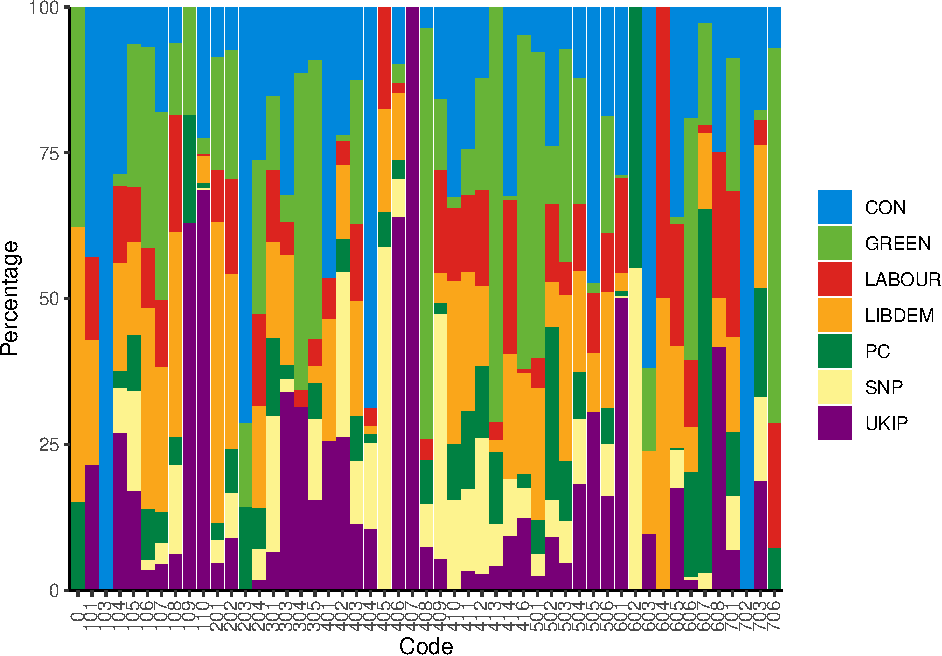
\includegraphics{_main_files/figure-latex/ggplot-nb-codes-1.pdf}

Now, we can see that some parties dominate some categories, while for others the spread is more even. For example, UKIP dominates the categories 406 and 407 - dealing with positive and negative mentions of protectionism, while the Conservatives do the same with category 103 (\emph{Anti-Imperialism}). Note though, that these are percentages. This means that the reason the Conservatives dominate category 103 is as they have two (quasi)-sentences with that category. The others do not have the category at all (702 on \emph{Negative Mentioning of Labour Groups} has the same issue). Other categories, such as 403 (\emph{Market Regulation}) and 502 (\emph{Positive Mentions of Culture}) are way better spread out over all the parties.

Another thing we can look at is what part of a party's manifesto belongs to any of the codes. This can help us answer the question: ``what are the parties talking about?'' To see this, we have to calculate the column percentages:

\begin{Shaded}
\begin{Highlighting}[]
\NormalTok{prop\_col }\OtherTok{\textless{}{-}} \FunctionTok{as.data.frame}\NormalTok{((}\FunctionTok{prop.table}\NormalTok{(}\FunctionTok{table}\NormalTok{(manifesto\_data}\SpecialCharTok{$}\NormalTok{cmp\_code,manifesto\_data}\SpecialCharTok{$}\NormalTok{party), }\DecValTok{2}\NormalTok{) }\SpecialCharTok{*} \DecValTok{100}\NormalTok{))}
\FunctionTok{names}\NormalTok{(prop\_col) }\OtherTok{\textless{}{-}} \FunctionTok{c}\NormalTok{(}\StringTok{"Code"}\NormalTok{, }\StringTok{"Party"}\NormalTok{, }\StringTok{"Percentage"}\NormalTok{)}
\end{Highlighting}
\end{Shaded}

If we now type \texttt{prop\_col}, we can see what percentage of a party manifesto was about a certain code. Yet, given that there are 57 possible codes, it is more practical to cluster these in some way. Here, we do this using the Domains to which they belonged in the codebook. In total there are 7 domains (\url{https://manifesto-project.wzb.eu/down/papers/handbook_2014_version_5.pdf}), and a category that contains the 0 code. To cluster the codes, we make a new variable called \texttt{Domain}. To do so, we first transform the codes into a numeric format, create an empty variable called \texttt{Domain}, and then replace the NA values in this empty category with the name of the domain based on the values in the Code variable. This we do using various operators R uses: \texttt{\textgreater{}=} means greater than and equal to, while \texttt{\textless{}=} means smaller than and equal to. Then, we make this new variable into a factor, and sort this factor in the way the codes occur:

\begin{Shaded}
\begin{Highlighting}[]
\NormalTok{prop\_col}\SpecialCharTok{$}\NormalTok{Code }\OtherTok{\textless{}{-}} \FunctionTok{as.numeric}\NormalTok{(}\FunctionTok{as.character}\NormalTok{(prop\_col}\SpecialCharTok{$}\NormalTok{Code))}
\NormalTok{prop\_col}\SpecialCharTok{$}\NormalTok{Domain }\OtherTok{\textless{}{-}} \ConstantTok{NA}

\NormalTok{prop\_col}\SpecialCharTok{$}\NormalTok{Domain[prop\_col}\SpecialCharTok{$}\NormalTok{Code }\SpecialCharTok{\textgreater{}=} \DecValTok{101} \SpecialCharTok{\&}\NormalTok{ prop\_col}\SpecialCharTok{$}\NormalTok{Code }\SpecialCharTok{\textless{}=} \DecValTok{110}\NormalTok{] }\OtherTok{\textless{}{-}} \StringTok{"External Relations"}
\NormalTok{prop\_col}\SpecialCharTok{$}\NormalTok{Domain[prop\_col}\SpecialCharTok{$}\NormalTok{Code }\SpecialCharTok{\textgreater{}=} \DecValTok{201} \SpecialCharTok{\&}\NormalTok{ prop\_col}\SpecialCharTok{$}\NormalTok{Code }\SpecialCharTok{\textless{}=} \DecValTok{204}\NormalTok{] }\OtherTok{\textless{}{-}} \StringTok{"Freedom and Democracy"}
\NormalTok{prop\_col}\SpecialCharTok{$}\NormalTok{Domain[prop\_col}\SpecialCharTok{$}\NormalTok{Code }\SpecialCharTok{\textgreater{}=} \DecValTok{301} \SpecialCharTok{\&}\NormalTok{ prop\_col}\SpecialCharTok{$}\NormalTok{Code }\SpecialCharTok{\textless{}=} \DecValTok{305}\NormalTok{] }\OtherTok{\textless{}{-}} \StringTok{"Political System"}
\NormalTok{prop\_col}\SpecialCharTok{$}\NormalTok{Domain[prop\_col}\SpecialCharTok{$}\NormalTok{Code }\SpecialCharTok{\textgreater{}=} \DecValTok{401} \SpecialCharTok{\&}\NormalTok{ prop\_col}\SpecialCharTok{$}\NormalTok{Code }\SpecialCharTok{\textless{}=} \DecValTok{416}\NormalTok{] }\OtherTok{\textless{}{-}} \StringTok{"Economy"}
\NormalTok{prop\_col}\SpecialCharTok{$}\NormalTok{Domain[prop\_col}\SpecialCharTok{$}\NormalTok{Code }\SpecialCharTok{\textgreater{}=} \DecValTok{501} \SpecialCharTok{\&}\NormalTok{ prop\_col}\SpecialCharTok{$}\NormalTok{Code }\SpecialCharTok{\textless{}=} \DecValTok{507}\NormalTok{] }\OtherTok{\textless{}{-}} \StringTok{"Welfare and Quality of Life"}
\NormalTok{prop\_col}\SpecialCharTok{$}\NormalTok{Domain[prop\_col}\SpecialCharTok{$}\NormalTok{Code }\SpecialCharTok{\textgreater{}=} \DecValTok{601} \SpecialCharTok{\&}\NormalTok{ prop\_col}\SpecialCharTok{$}\NormalTok{Code }\SpecialCharTok{\textless{}=} \DecValTok{608}\NormalTok{] }\OtherTok{\textless{}{-}} \StringTok{"Fabric of Society"}
\NormalTok{prop\_col}\SpecialCharTok{$}\NormalTok{Domain[prop\_col}\SpecialCharTok{$}\NormalTok{Code }\SpecialCharTok{\textgreater{}=} \DecValTok{701} \SpecialCharTok{\&}\NormalTok{ prop\_col}\SpecialCharTok{$}\NormalTok{Code }\SpecialCharTok{\textless{}=} \DecValTok{706}\NormalTok{] }\OtherTok{\textless{}{-}} \StringTok{"Social Groups"}
\NormalTok{prop\_col}\SpecialCharTok{$}\NormalTok{Domain[prop\_col}\SpecialCharTok{$}\NormalTok{Code }\SpecialCharTok{==} \DecValTok{0}\NormalTok{] }\OtherTok{\textless{}{-}} \StringTok{"NA"}

\NormalTok{prop\_col}\SpecialCharTok{$}\NormalTok{Domain }\OtherTok{\textless{}{-}} \FunctionTok{as.factor}\NormalTok{(prop\_col}\SpecialCharTok{$}\NormalTok{Domain)}
\NormalTok{prop\_col}\SpecialCharTok{$}\NormalTok{Domain }\OtherTok{\textless{}{-}} \FunctionTok{factor}\NormalTok{(prop\_col}\SpecialCharTok{$}\NormalTok{Domain,}\FunctionTok{levels}\NormalTok{(prop\_col}\SpecialCharTok{$}\NormalTok{Domain)[}\FunctionTok{c}\NormalTok{(}\DecValTok{2}\NormalTok{,}\DecValTok{4}\NormalTok{,}\DecValTok{6}\NormalTok{,}\DecValTok{1}\NormalTok{,}\DecValTok{8}\NormalTok{,}\DecValTok{3}\NormalTok{,}\DecValTok{7}\NormalTok{,}\DecValTok{5}\NormalTok{)])}
\end{Highlighting}
\end{Shaded}

We then construct a plot as we did above:

\begin{Shaded}
\begin{Highlighting}[]
\FunctionTok{ggplot}\NormalTok{(}\AttributeTok{data=}\NormalTok{prop\_col, }\FunctionTok{aes}\NormalTok{(}\AttributeTok{x=}\NormalTok{Party, }\AttributeTok{y=}\NormalTok{Percentage, }\AttributeTok{fill=}\NormalTok{Domain)) }\SpecialCharTok{+}
 \FunctionTok{geom\_bar}\NormalTok{(}\AttributeTok{stat =} \StringTok{"identity"}\NormalTok{, }\AttributeTok{position =} \StringTok{"stack"}\NormalTok{) }\SpecialCharTok{+}
 \FunctionTok{scale\_y\_continuous}\NormalTok{(}\AttributeTok{expand =} \FunctionTok{c}\NormalTok{(}\DecValTok{0}\NormalTok{,}\DecValTok{0}\NormalTok{)) }\SpecialCharTok{+}
 \FunctionTok{theme\_classic}\NormalTok{()}\SpecialCharTok{+}
 \FunctionTok{theme}\NormalTok{(}\AttributeTok{axis.text.x =} \FunctionTok{element\_text}\NormalTok{(}\AttributeTok{angle =} \DecValTok{90}\NormalTok{))}\SpecialCharTok{+}
 \FunctionTok{theme}\NormalTok{(}\AttributeTok{axis.text.x =} \FunctionTok{element\_text}\NormalTok{(}\AttributeTok{vjust =} \FloatTok{0.40}\NormalTok{))}
\end{Highlighting}
\end{Shaded}

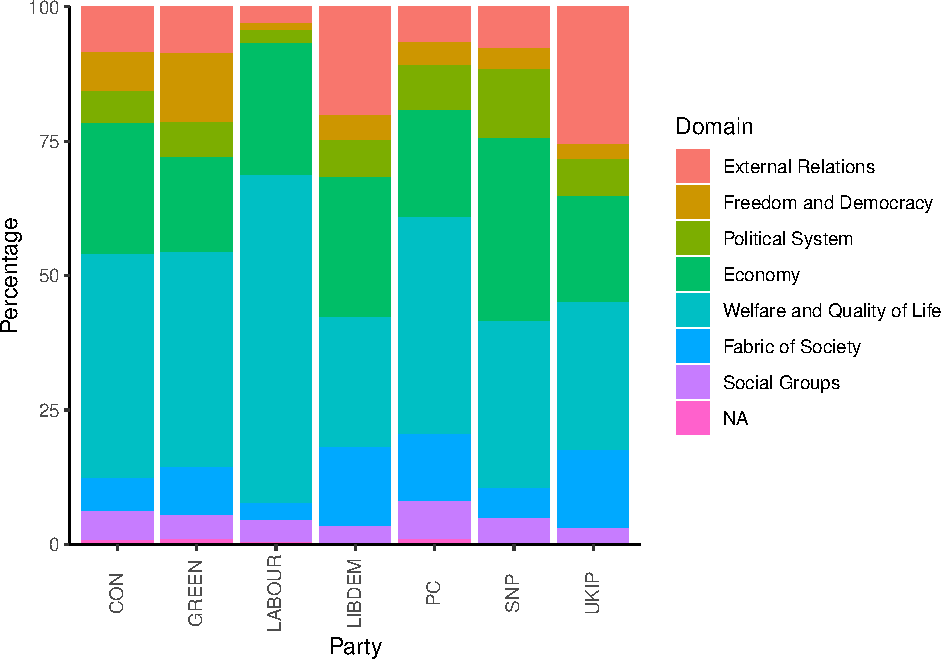
\includegraphics{_main_files/figure-latex/ggplot-nb-domains-1.pdf}

Here, we see that the Domain of \emph{Welfare and Quality of Life} was the most dominant in all the manifestos, with the \emph{Economy} coming second. Also, especially UKIP paid a lot of attention to \emph{External Relations}, while the Green party paid little attention to the \emph{Fabric of Society}. In all, this gives us a good idea of what type of data we are dealing with.

Now let's get back to the classification. For this, we need to transform the corpus from the \texttt{manifestoR} package into a corpus for the \texttt{quanteda} package. To do so, we first have to transform the former into a data frame, and then turn it into a corpus. We then look at the first 10 entries:

\begin{Shaded}
\begin{Highlighting}[]
\NormalTok{corpus\_data }\OtherTok{\textless{}{-}} \FunctionTok{mp\_corpus}\NormalTok{(manifestos) }\SpecialCharTok{\%\textgreater{}\%} 
 \FunctionTok{as.data.frame}\NormalTok{(}\AttributeTok{with.meta=}\ConstantTok{TRUE}\NormalTok{)}

\NormalTok{manifesto\_corpus }\OtherTok{\textless{}{-}} \FunctionTok{corpus}\NormalTok{(corpus\_data)}

\FunctionTok{summary}\NormalTok{(manifesto\_corpus, }\DecValTok{10}\NormalTok{)}
\end{Highlighting}
\end{Shaded}

Here, we see that the corpus treats each sentence as a separate document (which is confusing). We can still identify to which party they belong due to the \texttt{party} variable, which shows the party code. The \texttt{cmp\_code} variable shows the code assigned to the sentence (here it is all NA as the first sentences have the 0 category). To run the NB, instead of providing our training documents using a vector with NA values, we have to split our data set into a training and a test set. For this, we first generate a string of 8000 random numbers between 0 and 10780 (the total number of sentences). We do so to prevent our training or test set to exist only of sentences from a single party document:

\begin{Shaded}
\begin{Highlighting}[]
\FunctionTok{set.seed}\NormalTok{(}\DecValTok{42}\NormalTok{)}
\NormalTok{id\_train }\OtherTok{\textless{}{-}} \FunctionTok{sample}\NormalTok{(}\DecValTok{1}\SpecialCharTok{:}\DecValTok{10780}\NormalTok{, }\DecValTok{8000}\NormalTok{, }\AttributeTok{replace =} \ConstantTok{FALSE}\NormalTok{)}
\FunctionTok{head}\NormalTok{(id\_train, }\DecValTok{10}\NormalTok{)}
\end{Highlighting}
\end{Shaded}

\begin{verbatim}
##  [1]  2369  5273  9290  1252  8826 10289   356  7700  3954 10095
\end{verbatim}

Then we generate a unique number for each of the 10780 sentences in our corpus. This so we can later match them to the sentences we would like to place in our training set or our test set:

\begin{Shaded}
\begin{Highlighting}[]
\FunctionTok{docvars}\NormalTok{(manifesto\_corpus, }\StringTok{"id\_numeric"}\NormalTok{) }\OtherTok{\textless{}{-}} \DecValTok{1}\SpecialCharTok{:}\FunctionTok{ndoc}\NormalTok{(manifesto\_corpus)}
\end{Highlighting}
\end{Shaded}

We should now see this new variable \texttt{id\_numeric} appear in our corpus. We can now construct our training and test set using these id's. For the training set, the logic is to create a subset of the main corpus and to take only those sentences whose \texttt{id\_numeric} is also in \texttt{id\_train}. For the test set, we do the same, only now taking only those sentences whose \texttt{id\_numeric} is not in \texttt{id\_train} (note that the \texttt{!} mark signifies this). Then, we use the \texttt{\%\textgreater{}\%} pipe to transform the resulting object via a tokens object into a dfm:

\begin{Shaded}
\begin{Highlighting}[]
\NormalTok{manifesto\_train }\OtherTok{\textless{}{-}} \FunctionTok{corpus\_subset}\NormalTok{(manifesto\_corpus, id\_numeric }\SpecialCharTok{\%in\%}\NormalTok{ id\_train) }\SpecialCharTok{\%\textgreater{}\%}
 \FunctionTok{tokens}\NormalTok{() }\SpecialCharTok{\%\textgreater{}\%}
 \FunctionTok{dfm}\NormalTok{()}

\NormalTok{manifesto\_test }\OtherTok{\textless{}{-}} \FunctionTok{corpus\_subset}\NormalTok{(manifesto\_corpus, }\SpecialCharTok{!}\NormalTok{id\_numeric }\SpecialCharTok{\%in\%}\NormalTok{ id\_train) }\SpecialCharTok{\%\textgreater{}\%}
 \FunctionTok{tokens}\NormalTok{() }\SpecialCharTok{\%\textgreater{}\%}
 \FunctionTok{dfm}\NormalTok{()}
\end{Highlighting}
\end{Shaded}

We then run the model using the \texttt{textmodel\_nb} command, and ask it to use as classifiers the codes in the \texttt{cmp\_code} variable:

\begin{Shaded}
\begin{Highlighting}[]
\NormalTok{manifesto\_nb }\OtherTok{\textless{}{-}} \FunctionTok{textmodel\_nb}\NormalTok{(manifesto\_train, }\FunctionTok{docvars}\NormalTok{(manifesto\_train, }\StringTok{"cmp\_code"}\NormalTok{))}
\FunctionTok{summary}\NormalTok{(manifesto\_nb)}
\end{Highlighting}
\end{Shaded}

Notice that this command gives us a prediction of how likely it is that an individual word belongs to a certain code (the estimated feature scores). While this can be interesting, what we want to know here is how good the algorithm was. This is when we move from the training of the model using the training set to the prediction of the test set.

A problem is that Naive Bayes can only use features that were both in the training and the test set. To ensure this happens, we use the \texttt{dfm\_match} option, which matches all the features in our dfm to a specified vector of features:

\begin{Shaded}
\begin{Highlighting}[]
\NormalTok{manifesto\_matched }\OtherTok{\textless{}{-}} \FunctionTok{dfm\_match}\NormalTok{(manifesto\_test, }\AttributeTok{features =} \FunctionTok{featnames}\NormalTok{(manifesto\_train))}
\end{Highlighting}
\end{Shaded}

If we look at this new corpus we see that little has changed (there are still 2780 features). This means that all features that were in the test set were also there in the training set. This is good news as this means the algorithm has all the information needed for a good prediction. Yet, the lower the number of sentences, the less likely this is to occur, so matching is always a good idea.

Now we can predict the missing codes in the test set (now the manifesto\_matched dfm) using the model we trained earlier. The resulting classes are what the model predicts (we already set this when we trained the model). If we would then open the \texttt{predicted\_class} object we can see to which code R assigned each sentence. Yet, as before, this is a little too much information. Moreover, we do not want to know what the model assigned the sentence to, but how this corresponds to the original code. To see this, we take the actual classes from the \texttt{manifesto\_matched} dfm and place them with the predicted classes into a cross table:

\begin{Shaded}
\begin{Highlighting}[]
\NormalTok{predicted\_class }\OtherTok{\textless{}{-}} \FunctionTok{predict}\NormalTok{(manifesto\_nb, }\AttributeTok{newdata =}\NormalTok{ manifesto\_matched)}
\NormalTok{actual\_class }\OtherTok{\textless{}{-}} \FunctionTok{docvars}\NormalTok{(manifesto\_matched, }\StringTok{"cmp\_code"}\NormalTok{)}
\NormalTok{table\_class }\OtherTok{\textless{}{-}} \FunctionTok{table}\NormalTok{(actual\_class, predicted\_class)}
\NormalTok{table\_class}
\end{Highlighting}
\end{Shaded}

While this is already better (we have to pay attention to the diagonal), the large number of codes still makes this hard to read. So, as before, we can better visualise these results - here with the help of a heatmap. To do this, we first transform our table into a data frame that gives us all the possible combinations of codes and their occurrence. We put this into the command and also use a scaling gradient that gets darker when the value in a cell is higher:

\begin{Shaded}
\begin{Highlighting}[]
\NormalTok{table\_class }\OtherTok{\textless{}{-}} \FunctionTok{as.data.frame}\NormalTok{(table\_class)}

\FunctionTok{ggplot}\NormalTok{(}\AttributeTok{data =}\NormalTok{ table\_class, }\FunctionTok{aes}\NormalTok{(}\AttributeTok{x =}\NormalTok{ predicted\_class, }\AttributeTok{y =}\NormalTok{ actual\_class)) }\SpecialCharTok{+}
 \FunctionTok{geom\_tile}\NormalTok{(}\FunctionTok{aes}\NormalTok{(}\AttributeTok{fill =}\NormalTok{ Freq)) }\SpecialCharTok{+}
 \FunctionTok{scale\_fill\_gradient}\NormalTok{(}\AttributeTok{high =} \StringTok{"black"}\NormalTok{, }\AttributeTok{low =} \StringTok{"white"}\NormalTok{, }\AttributeTok{name=}\StringTok{"Value"}\NormalTok{)}\SpecialCharTok{+}
 \FunctionTok{xlab}\NormalTok{(}\StringTok{"Predicted Class"}\NormalTok{)}\SpecialCharTok{+}
 \FunctionTok{ylab}\NormalTok{(}\StringTok{"Actual Class"}\NormalTok{)}\SpecialCharTok{+}
 \FunctionTok{scale\_y\_discrete}\NormalTok{(}\AttributeTok{expand =} \FunctionTok{c}\NormalTok{(}\DecValTok{0}\NormalTok{,}\DecValTok{0}\NormalTok{)) }\SpecialCharTok{+}
 \FunctionTok{theme\_classic}\NormalTok{()}\SpecialCharTok{+}
 \FunctionTok{theme}\NormalTok{(}\AttributeTok{axis.text.x =} \FunctionTok{element\_text}\NormalTok{(}\AttributeTok{angle =} \DecValTok{90}\NormalTok{))}\SpecialCharTok{+}
 \FunctionTok{theme}\NormalTok{(}\AttributeTok{axis.text.x =} \FunctionTok{element\_text}\NormalTok{(}\AttributeTok{vjust =} \FloatTok{0.40}\NormalTok{))}
\end{Highlighting}
\end{Shaded}

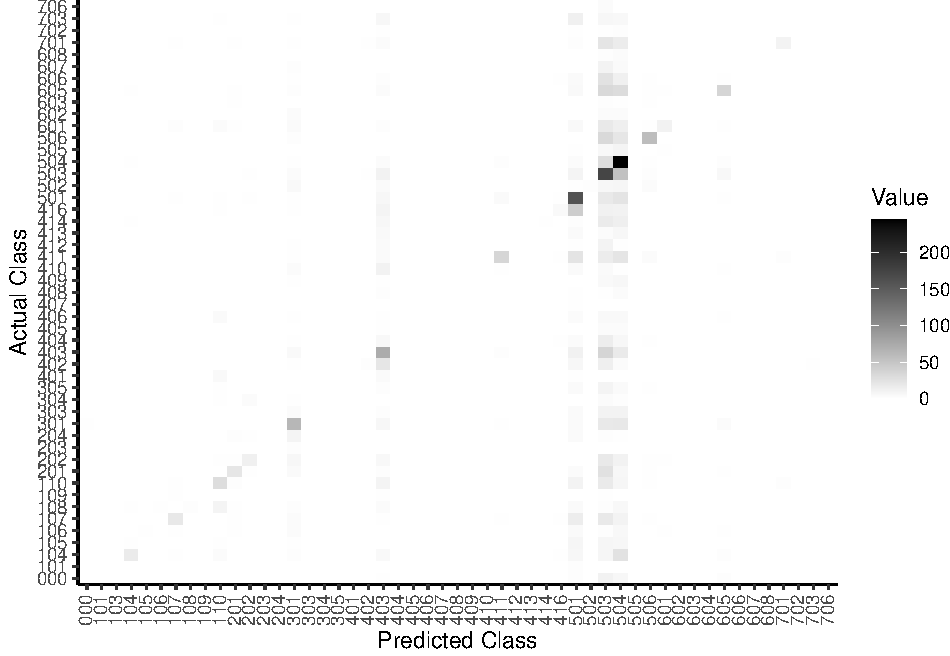
\includegraphics{_main_files/figure-latex/ggplot-nb-heatmap-1.pdf}

Here, we can see that a high number of cases are on the diagonal, which indicates that the algorithm did a good job. Yet, it also classified a large number of sentences into the 503 and 504 categories, while they belonged to any of the other categories.

Besides this, we can also summarize how good the algorithm is through Krippendorff's \(\alpha\). To do so, we take the predicted codes, transform them from factors to numeric values, and store them in an object. Then, we bind them together with the actual codes and place them into a data frame. Finally, we transpose the data frame (so that rows are now columns) and make it into a matrix:

\begin{Shaded}
\begin{Highlighting}[]
\NormalTok{predict }\OtherTok{\textless{}{-}} \FunctionTok{as.numeric}\NormalTok{(}\FunctionTok{as.character}\NormalTok{(predicted\_class))}
\NormalTok{reliability }\OtherTok{\textless{}{-}} \FunctionTok{as.data.frame}\NormalTok{(}\FunctionTok{cbind}\NormalTok{(actual\_class, predict))}
\NormalTok{reliability\_t }\OtherTok{\textless{}{-}} \FunctionTok{t}\NormalTok{(reliability)}
\NormalTok{reliability }\OtherTok{\textless{}{-}} \FunctionTok{as.matrix}\NormalTok{(reliability\_t)}
\end{Highlighting}
\end{Shaded}

Then, we load the \texttt{kripp.boot} package, and calculate the nominal version of Krippendorff's \(\alpha\), as we are working with nominal codes:

\begin{Shaded}
\begin{Highlighting}[]
\FunctionTok{library}\NormalTok{(kripp.boot)}
\FunctionTok{kripp.boot}\NormalTok{(reliability, }\AttributeTok{iter =} \DecValTok{500}\NormalTok{, }\AttributeTok{method =} \StringTok{"nominal"}\NormalTok{)}
\end{Highlighting}
\end{Shaded}

As an alternative, we can use the \texttt{DescTools} package:

\begin{Shaded}
\begin{Highlighting}[]
\FunctionTok{library}\NormalTok{(DescTools)}
\FunctionTok{KrippAlpha}\NormalTok{(reliability, }\AttributeTok{method =} \StringTok{"nominal"}\NormalTok{)}
\end{Highlighting}
\end{Shaded}

Here we see that the number of subjects was 2780 (the number of sentences in the test set), the number of coders 2 (the actual and the predicted codes), and the value of \(\alpha\) 0.318 with an interval between 0.297 and 0.337. While this might not look particularly encouraging, when we realise that Mikhaylov et al. (\citeproc{ref-Mikhaylov2012a}{2012}) estimate the agreement among trained coders by the Manifesto Project to be between 0.350 and 0.400, then 0.305 is quite a good score for a simple model!

\chapter{Unsupervised Methods}\label{unsupervised-methods}

While supervised models often work fine for text classification, one disadvantage is that we need to set specifics for the model. As an alternative, we can not specify anything and have R find out which classifications work. There are various algorithms to do so, of which we here will focus on Latent Dirichlet Allocation (LDA); a `seeded' version of LDA that uses information from other sources to improve the results of the LDA; and a Structural Topic Model.

\section{Latent Dirichlet Allocation}\label{latent-dirichlet-allocation}

Latent Dirichlet Allocation, or LDA, relies on the idea is that each text is a mix of topics, and each word belongs to one of these. To run LDA, we will use the \texttt{topicmodels} package, and use the inaugural speeches as an example. First, we will use the \texttt{convert} function to convert the data frequency matrix to a data term matrix as this is what \texttt{topicmodels} uses:

\begin{Shaded}
\begin{Highlighting}[]
\FunctionTok{library}\NormalTok{(topicmodels)}
\NormalTok{inaugural\_dtm }\OtherTok{\textless{}{-}} \FunctionTok{convert}\NormalTok{(data\_inaugural\_dfm, }\AttributeTok{to =} \StringTok{"topicmodels"}\NormalTok{)}
\end{Highlighting}
\end{Shaded}

Then, we fit an LDA model with 10 topics. First, we have to define some a priori parameters for the model. Here, we will use the Gibbs sampling method to fit the LDA model (\citeproc{ref-Griffiths2004a}{Griffiths \& Steyvers, 2004}) over the alternative VEM approach (\citeproc{ref-Blei2003a}{Blei et al., 2003}). Gibbs sampling performs a random walk over the distribution so we need to set a seed to ensure reproducible results. In this particular example, we set five seeds for five independent runs. We also set a burn-in period of 2000 as the first iterations will not reflect the distribution well, and take the 200th iteration of the following 1000:

\begin{Shaded}
\begin{Highlighting}[]
\NormalTok{burnin }\OtherTok{\textless{}{-}} \DecValTok{2000}
\NormalTok{iter }\OtherTok{\textless{}{-}} \DecValTok{1000}
\NormalTok{thin }\OtherTok{\textless{}{-}} \DecValTok{200}
\NormalTok{seed }\OtherTok{\textless{}{-}} \FunctionTok{list}\NormalTok{(}\DecValTok{42}\NormalTok{,}\DecValTok{5}\NormalTok{,}\DecValTok{24}\NormalTok{,}\DecValTok{158}\NormalTok{,}\DecValTok{2500}\NormalTok{)}
\NormalTok{nstart }\OtherTok{\textless{}{-}} \DecValTok{5}
\NormalTok{best }\OtherTok{\textless{}{-}} \ConstantTok{TRUE}
\end{Highlighting}
\end{Shaded}

The LDA algorithm estimates topic-word probabilities as well as topic-document probabilities that we can extract and visualize. Here, we will start with the topic-word probabilities called \texttt{beta}. To do this, we will use the \texttt{tidytext} package which is part of the tidyverse family of packages. Central to the logic of tidyverse packages is that it does not rely on a document term matrix but represents the data in a long format (\citeproc{ref-Welbers2017a}{Welbers et al., 2017, p. 252}). Although this makes it less memory efficient, this lends itself to effective visualisation. The whole logic of these packages is that it works with data which has columns (variables) and rows with single observations. While this is the logic most people know, but it is not always the quickest (and is also not used by \texttt{quanteda}). Yet, it always allows you to look at your data in a way most will understand. First, we run the LDA and have a look at the first 10 terms:

\begin{Shaded}
\begin{Highlighting}[]
\NormalTok{inaugural\_lda10 }\OtherTok{\textless{}{-}} \FunctionTok{LDA}\NormalTok{(inaugural\_dtm, }\AttributeTok{k=}\DecValTok{10}\NormalTok{,}
                       \AttributeTok{method=}\StringTok{"Gibbs"}\NormalTok{,}
                       \AttributeTok{control=}\FunctionTok{list}\NormalTok{(}\AttributeTok{burnin=}\NormalTok{burnin,}
                                    \AttributeTok{iter=}\NormalTok{iter,}
                                    \AttributeTok{thin=}\NormalTok{thin,}
                                    \AttributeTok{seed=}\NormalTok{seed,}
                                    \AttributeTok{nstart=}\NormalTok{nstart,}
                                    \AttributeTok{best=}\NormalTok{best))}

\FunctionTok{terms}\NormalTok{(inaugural\_lda10, }\DecValTok{10}\NormalTok{)}
\end{Highlighting}
\end{Shaded}

\begin{verbatim}
##       Topic 1      Topic 2    Topic 3     Topic 4     Topic 5   Topic 6    
##  [1,] "government" "nations"  "women"     "business"  "us"      "freedom"  
##  [2,] "justice"    "world"    "love"      "race"      "can"     "liberty"  
##  [3,] "progress"   "peace"    "many"      "may"       "new"     "every"    
##  [4,] "system"     "free"     "much"      "necessary" "nation"  "americans"
##  [5,] "laws"       "freedom"  "days"      "made"      "america" "still"    
##  [6,] "greater"    "peoples"  "story"     "passed"    "must"    "rights"   
##  [7,] "economic"   "may"      "moment"    "proper"    "world"   "care"     
##  [8,] "prosperity" "people"   "like"      "tariff"    "people"  "came"     
##  [9,] "public"     "strength" "americans" "feeling"   "time"    "states"   
## [10,] "many"       "united"   "thank"     "increase"  "one"     "ideals"   
##       Topic 7      Topic 8    Topic 9      Topic 10       
##  [1,] "can"        "life"     "man"        "republic"     
##  [2,] "must"       "upon"     "change"     "never"        
##  [3,] "government" "men"      "earth"      "war"          
##  [4,] "upon"       "shall"    "done"       "may"          
##  [5,] "law"        "purpose"  "believe"    "must"         
##  [6,] "shall"      "good"     "seek"       "civilization" 
##  [7,] "congress"   "great"    "economy"    "lies"         
##  [8,] "country"    "without"  "generation" "order"        
##  [9,] "people"     "problems" "union"      "understanding"
## [10,] "states"     "duty"     "small"      "sound"
\end{verbatim}

Here, we can see that the first topic is most concerned with words referring to peace and freedom, the second with references to the people, the third with businesses, as so on. While we can interpret our topics this way, a better way might be to visualise the results. For this, we will use the \texttt{tidy} command to prepare the dataset for visualisation. Then, we tell the command to use the information from the \texttt{beta} column, which contains the probability of a word occurring in a certain topic:

\begin{Shaded}
\begin{Highlighting}[]
\FunctionTok{library}\NormalTok{(tidytext)}
\FunctionTok{library}\NormalTok{(dplyr)}
\FunctionTok{library}\NormalTok{(ggplot2)}

\NormalTok{inaugural\_lda10\_topics }\OtherTok{\textless{}{-}} \FunctionTok{tidy}\NormalTok{(inaugural\_lda10, }\AttributeTok{matrix=}\StringTok{"beta"}\NormalTok{)}
\end{Highlighting}
\end{Shaded}

If we would look into the dataset now, we would see that it has 63130 observations with 3 variables. These are the number of the topic, the word (the term) and the \texttt{beta} - the chance that the word occurs in that topic. We now want to visualise only the top ten words for each topic in a bar plot. Also, we want the graphs of each of these ten topics to appear in a single graph. To make this happen, we first have to select the top ten words for each topic. We do so again using a pipe (which is the \texttt{\%\textgreater{}\%} command). This pipe transports an output of a command to another one before saving it. So here, we take our data set and group it by topic using the \texttt{group\_by} command. This command groups the dataset into 10 groups, each for every topic. What this allows us is to calculate things that we otherwise calculate for the whole data-set but here calculate for the groups instead. We then do so and select the top 10 terms (based on their beta value), using \texttt{top\_n}. We then ungroup again (to make R view it as a single data-set), and use the \texttt{arrange} function to ensure the data-set sorts the topics in an increasing and the beta values in a decreasing fashion. Finally, we save this into a new object:

\begin{Shaded}
\begin{Highlighting}[]
\NormalTok{inaugural\_lda10\_topterms }\OtherTok{\textless{}{-}}\NormalTok{ inaugural\_lda10\_topics }\SpecialCharTok{\%\textgreater{}\%}
 \FunctionTok{group\_by}\NormalTok{(topic) }\SpecialCharTok{\%\textgreater{}\%}
 \FunctionTok{top\_n}\NormalTok{(}\DecValTok{10}\NormalTok{, beta) }\SpecialCharTok{\%\textgreater{}\%}
 \FunctionTok{ungroup}\NormalTok{() }\SpecialCharTok{\%\textgreater{}\%}
 \FunctionTok{arrange}\NormalTok{(topic, }\SpecialCharTok{{-}}\NormalTok{beta)}
\end{Highlighting}
\end{Shaded}

If we now look at the data set, we see that it is much smaller and has the topics ordered. Yet, before we can plot this we have to ensure that (seen from top to bottom), all the beta for the first topic come first, then for the second topic, and so on. To do so, we use the \texttt{mutate} command, and redefine the term variable so that it is re-ordered based first on the term and then on the beta value. The result is a data frame with first the first topic, then the second topic etc., and with the beta values ordered within each topic. We then make the figure, with the terms on the horizontal axis and the beta values and the vertical axes, and have the bars this generates coloured by topic. Also, we switch off the legend (which we do not need) and use the \texttt{facet\_wrap} command to split up the total graph (which would have 107 bars otherwise - 107 bars and not a 100 because some terms had the same value for beta). We set the options for the scales to be \texttt{free} as it might be that the beta values for some topics are larger or smaller than for the others. Finally, we flip the graphs and make the x-axis the y-axis and vice versa, as this makes the picture more clear:

\begin{Shaded}
\begin{Highlighting}[]
\NormalTok{inaugural\_lda10\_topterms }\SpecialCharTok{\%\textgreater{}\%}
 \FunctionTok{mutate}\NormalTok{(}\AttributeTok{term=}\FunctionTok{reorder}\NormalTok{(term, beta)) }\SpecialCharTok{\%\textgreater{}\%}
 \FunctionTok{ggplot}\NormalTok{(}\FunctionTok{aes}\NormalTok{(term, beta, }\AttributeTok{fill=}\FunctionTok{factor}\NormalTok{(topic))) }\SpecialCharTok{+}
 \FunctionTok{geom\_col}\NormalTok{(}\AttributeTok{show.legend=}\ConstantTok{FALSE}\NormalTok{) }\SpecialCharTok{+}
 \FunctionTok{facet\_wrap}\NormalTok{(}\SpecialCharTok{\textasciitilde{}}\NormalTok{ topic, }\AttributeTok{scales=}\StringTok{"free"}\NormalTok{) }\SpecialCharTok{+}
 \FunctionTok{coord\_flip}\NormalTok{()}\SpecialCharTok{+}
 \FunctionTok{theme\_minimal}\NormalTok{()}
\end{Highlighting}
\end{Shaded}

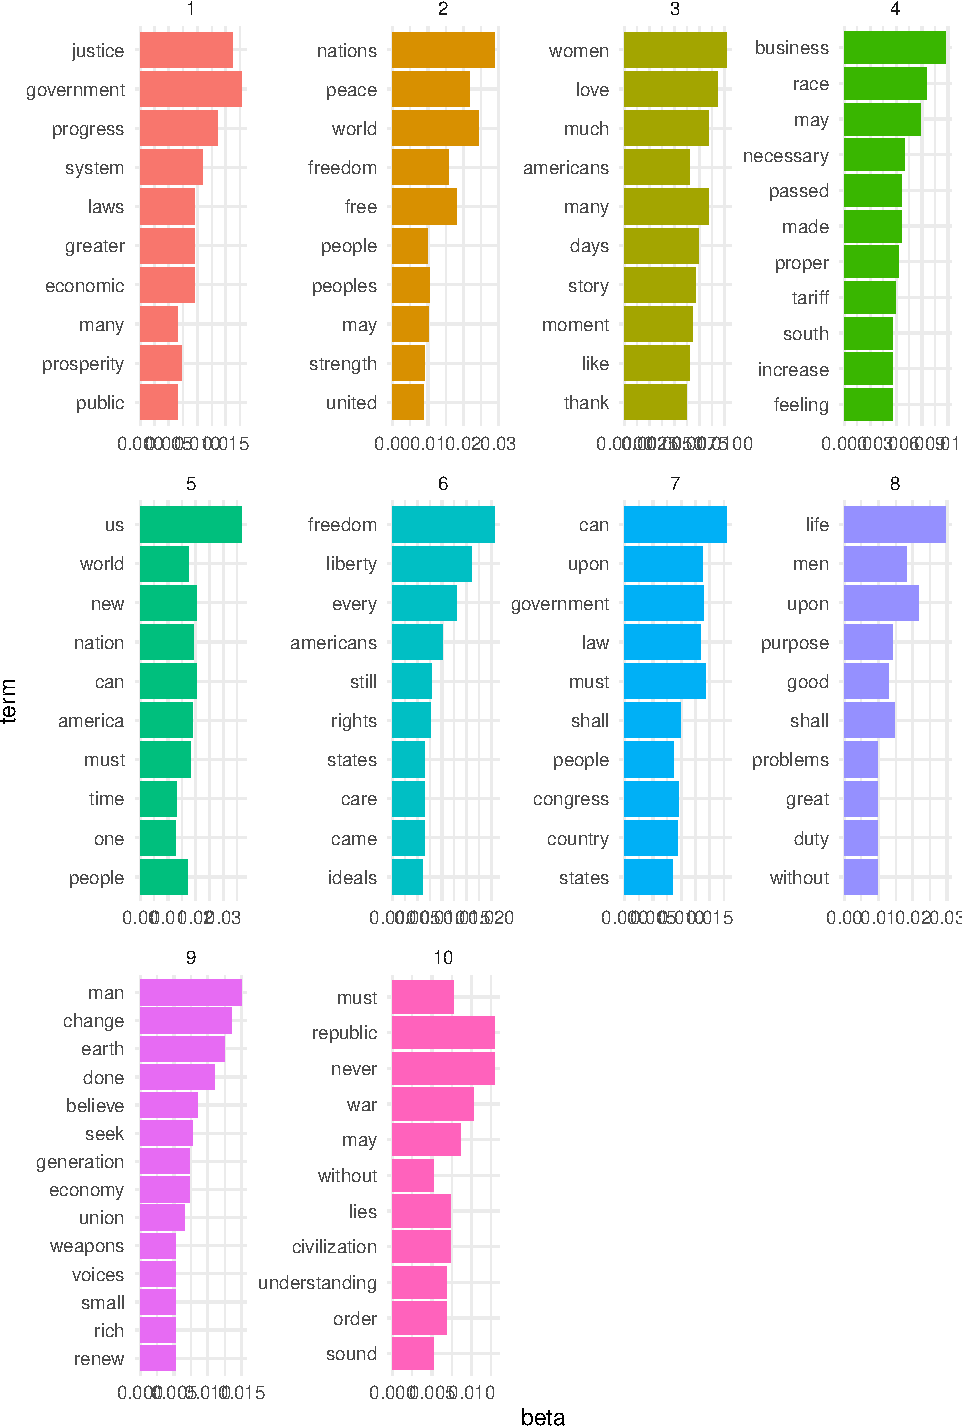
\includegraphics{_main_files/figure-latex/lda-tidy-graph1-1.pdf}

What is clear here is that looking at only the words in each topic only says so much. In the first topic, the term `peace' is more important than anything else, and so is `us' in topic number 2. Also, in topic number ten, we see that both `first' and `need' are of equal importance.

Another question we can ask is how much of each topic is in each of the documents. Put in another way: do certain documents talk more about certain topics than others? To see this, we first generate a new data frame with this information, known as the \texttt{gamma} value for each document:

\begin{Shaded}
\begin{Highlighting}[]
\NormalTok{inaugural\_lda10\_documents }\OtherTok{\textless{}{-}} \FunctionTok{tidy}\NormalTok{(inaugural\_lda10, }\AttributeTok{matrix=}\StringTok{"gamma"}\NormalTok{)}
\end{Highlighting}
\end{Shaded}

We then go through similar steps to make the data set ready for use and prepare the graph. For the graph, the only steps we do different are to force R to label each topic on the axis (as otherwise it will treat it as a continuous variable and come up with useless values such as 7.5), and to give it a different look (using the \texttt{theme\_classic()} command):

\begin{Shaded}
\begin{Highlighting}[]
\NormalTok{inaugural\_lda10\_toptopics }\OtherTok{\textless{}{-}}\NormalTok{ inaugural\_lda10\_documents }\SpecialCharTok{\%\textgreater{}\%}
 \FunctionTok{group\_by}\NormalTok{(document) }\SpecialCharTok{\%\textgreater{}\%}
 \FunctionTok{top\_n}\NormalTok{(}\DecValTok{10}\NormalTok{, gamma) }\SpecialCharTok{\%\textgreater{}\%}
 \FunctionTok{ungroup}\NormalTok{() }\SpecialCharTok{\%\textgreater{}\%}
 \FunctionTok{arrange}\NormalTok{(topic, }\SpecialCharTok{{-}}\NormalTok{gamma)}
\end{Highlighting}
\end{Shaded}

\begin{Shaded}
\begin{Highlighting}[]
\NormalTok{inaugural\_lda10\_toptopics }\SpecialCharTok{\%\textgreater{}\%}
 \FunctionTok{mutate}\NormalTok{(}\AttributeTok{term=}\FunctionTok{reorder}\NormalTok{(topic, gamma)) }\SpecialCharTok{\%\textgreater{}\%}
 \FunctionTok{ggplot}\NormalTok{(}\FunctionTok{aes}\NormalTok{(topic, gamma, }\AttributeTok{fill=}\FunctionTok{factor}\NormalTok{(topic))) }\SpecialCharTok{+}
 \FunctionTok{geom\_col}\NormalTok{(}\AttributeTok{show.legend=}\ConstantTok{FALSE}\NormalTok{) }\SpecialCharTok{+}
 \FunctionTok{scale\_x\_continuous}\NormalTok{(}\AttributeTok{breaks =} \FunctionTok{c}\NormalTok{(}\DecValTok{1}\NormalTok{,}\DecValTok{2}\NormalTok{,}\DecValTok{3}\NormalTok{,}\DecValTok{4}\NormalTok{,}\DecValTok{5}\NormalTok{,}\DecValTok{6}\NormalTok{,}\DecValTok{7}\NormalTok{,}\DecValTok{8}\NormalTok{,}\DecValTok{9}\NormalTok{,}\DecValTok{10}\NormalTok{))}\SpecialCharTok{+}
 \FunctionTok{facet\_wrap}\NormalTok{(}\SpecialCharTok{\textasciitilde{}}\NormalTok{ document, }\AttributeTok{scales=}\StringTok{"free"}\NormalTok{) }\SpecialCharTok{+}
 \FunctionTok{coord\_flip}\NormalTok{()}\SpecialCharTok{+}
 \FunctionTok{theme\_minimal}\NormalTok{()}
\end{Highlighting}
\end{Shaded}

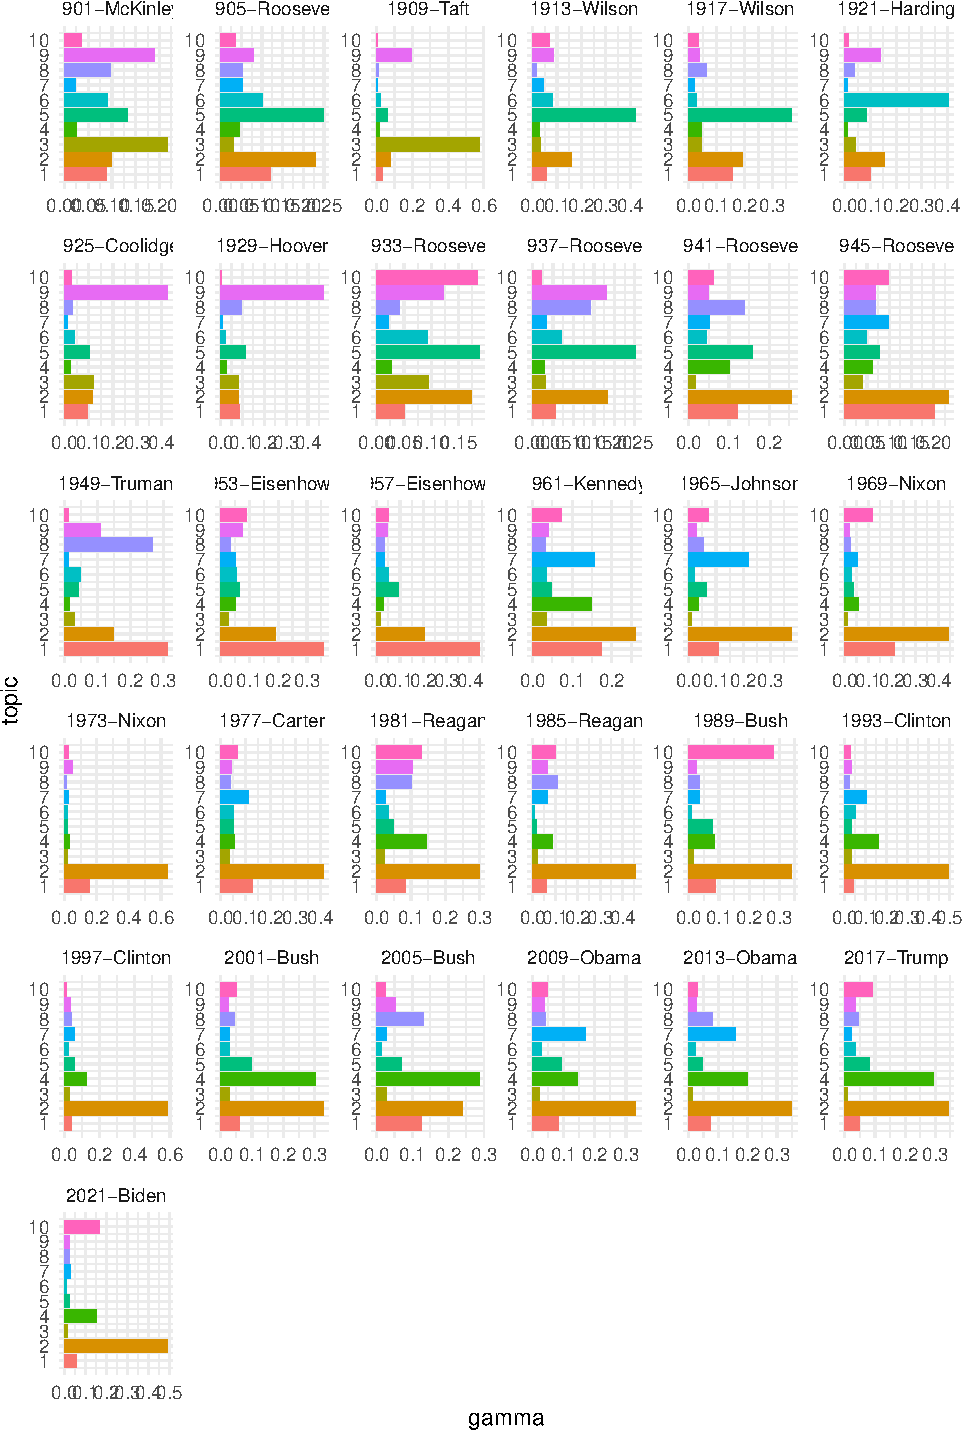
\includegraphics{_main_files/figure-latex/lda-tidy-graph2-1.pdf}

Here, we see that in 1929 Hoover talked most often about topic 9 (focusing on government), Biden in 2021 focused on words like `us' and `people', while in 1945 Roosevelt seemed to favour both the people and topics referring to peace. Again, our exact conclusions of course depend on how we interpret the topics.

\section{Seeded Latent Dirichlet Allocation}\label{seeded-latent-dirichlet-allocation}

An alternative to the above approach is one known as seeded-LDA. This approach uses seed words that can steer the LDA in the right direction. One origin of these seed words can be a dictionary that tells the algorithm which words belong together in various categories. To use it, we will first load the packages and set a seed:

\begin{Shaded}
\begin{Highlighting}[]
\FunctionTok{library}\NormalTok{(seededlda)}
\FunctionTok{library}\NormalTok{(quanteda.dictionaries)}

\FunctionTok{set.seed}\NormalTok{(}\DecValTok{42}\NormalTok{)}
\end{Highlighting}
\end{Shaded}

Next, we need to specify a selection of seed words in dictionary form. While we can construct a dictionary ourselves, here we choose to use the Laver and Garry dictionary we saw earlier. We then use this dictionary to run our seeded LDA:

\begin{Shaded}
\begin{Highlighting}[]
\NormalTok{dictionary\_LaverGarry }\OtherTok{\textless{}{-}} \FunctionTok{dictionary}\NormalTok{(data\_dictionary\_LaverGarry)}
\NormalTok{seededmodel }\OtherTok{\textless{}{-}} \FunctionTok{textmodel\_seededlda}\NormalTok{(data\_inaugural\_dfm, }\AttributeTok{dictionary =}\NormalTok{ dictionary\_LaverGarry)}
\FunctionTok{terms}\NormalTok{(seededmodel, }\DecValTok{20}\NormalTok{)}
\end{Highlighting}
\end{Shaded}

\begin{verbatim}
##       CULTURE     ECONOMY       ENVIRONMENT     GROUPS      INSTITUTIONS    
##  [1,] "people"    "work"        "civilization"  "women"     "president"     
##  [2,] "us"        "government"  "production"    "race"      "administration"
##  [3,] "new"       "can"         "productive"    "day"       "executive"     
##  [4,] "america"   "upon"        "republic"      "story"     "continue"      
##  [5,] "nation"    "great"       "population"    "thank"     "office"        
##  [6,] "world"     "must"        "war"           "back"      "business"      
##  [7,] "must"      "may"         "order"         "bless"     "congress"      
##  [8,] "can"       "shall"       "produce"       "president" "policy"        
##  [9,] "time"      "economic"    "tasks"         "schools"   "legislation"   
## [10,] "let"       "justice"     "planet"        "around"    "law"           
## [11,] "one"       "opportunity" "products"      "yes"       "modern"        
## [12,] "today"     "children"    "making"        "across"    "rule"          
## [13,] "now"       "country"     "conditions"    "hand"      "authority"     
## [14,] "every"     "united"      "productivity"  "left"      "race"          
## [15,] "make"      "war"         "relations"     "friends"   "necessary"     
## [16,] "americans" "progress"    "promote"       "began"     "agencies"      
## [17,] "american"  "men"         "maintained"    "lost"      "make"          
## [18,] "years"     "never"       "understanding" "racial"    "proper"        
## [19,] "together"  "economy"     "leadership"    "young"     "reforms"       
## [20,] "spirit"    "made"        "normal"        "founding"  "voices"        
##       LAW_AND_ORDER   RURAL           URBAN        VALUES      
##  [1,] "force"         "public"        "man"        "freedom"   
##  [2,] "determined"    "law"           "price"      "history"   
##  [3,] "forces"        "party"         "sides"      "human"     
##  [4,] "men"           "permanent"     "begin"      "peace"     
##  [5,] "determination" "toward"        "growth"     "free"      
##  [6,] "day"           "enforcement"   "loyalty"    "world"     
##  [7,] "court"         "agricultural"  "covenant"   "nations"   
##  [8,] "counsel"       "relations"     "sick"       "rights"    
##  [9,] "every"         "direction"     "compassion" "principles"
## [10,] "something"     "nation"        "final"      "past"      
## [11,] "evil"          "establishment" "heal"       "help"      
## [12,] "mind"          "islands"       "globe"      "life"      
## [13,] "conviction"    "countrymen"    "goals"      "faith"     
## [14,] "terror"        "stability"     "passed"     "strength"  
## [15,] "necessity"     "independence"  "call"       "live"      
## [16,] "life"          "feed"          "understood" "know"      
## [17,] "dealing"       "provided"      "suffer"     "peoples"   
## [18,] "body"          "civilization"  "trying"     "security"  
## [19,] "democratic"    "agriculture"   "mountains"  "humanity"  
## [20,] "determine"     "ideals"        "assure"     "leadership"
\end{verbatim}

Note that using the dictionary has ensured that we only use the categories that occur in the dictionary. This means that we can look at which topics are in each inaugural speech and which terms were most likely for each of the topics. Let us start with the topics first:

\begin{Shaded}
\begin{Highlighting}[]
\NormalTok{topics }\OtherTok{\textless{}{-}} \FunctionTok{topics}\NormalTok{(seededmodel)}
\NormalTok{topics\_table }\OtherTok{\textless{}{-}} \FunctionTok{ftable}\NormalTok{(topics)}
\NormalTok{topics\_prop\_table }\OtherTok{\textless{}{-}} \FunctionTok{as.data.frame}\NormalTok{(}\FunctionTok{prop.table}\NormalTok{(topics\_table))}

\FunctionTok{ggplot}\NormalTok{(}\AttributeTok{data=}\NormalTok{topics\_prop\_table, }\FunctionTok{aes}\NormalTok{(}\AttributeTok{x=}\NormalTok{topics, }\AttributeTok{y=}\NormalTok{Freq))}\SpecialCharTok{+}
 \FunctionTok{geom\_bar}\NormalTok{(}\AttributeTok{stat=}\StringTok{"identity"}\NormalTok{)}\SpecialCharTok{+}
 \FunctionTok{labs}\NormalTok{(}\AttributeTok{x=}\StringTok{"Topics"}\NormalTok{, }\AttributeTok{y=}\StringTok{"Topic Percentage"}\NormalTok{)}\SpecialCharTok{+}
 \FunctionTok{scale\_y\_continuous}\NormalTok{(}\AttributeTok{expand =} \FunctionTok{c}\NormalTok{(}\DecValTok{0}\NormalTok{, }\DecValTok{0}\NormalTok{)) }\SpecialCharTok{+}
 \FunctionTok{theme\_classic}\NormalTok{()}\SpecialCharTok{+}
 \FunctionTok{theme}\NormalTok{(}\AttributeTok{axis.text.x =} \FunctionTok{element\_text}\NormalTok{(}\AttributeTok{size=}\DecValTok{10}\NormalTok{, }\AttributeTok{angle=}\DecValTok{90}\NormalTok{, }\AttributeTok{hjust =} \DecValTok{1}\NormalTok{))}
\end{Highlighting}
\end{Shaded}

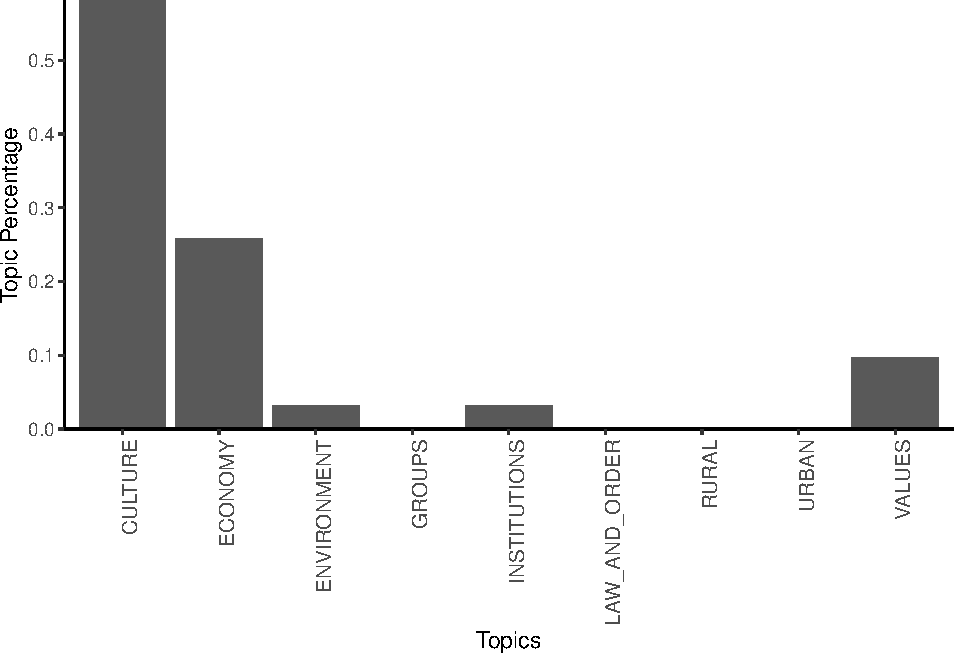
\includegraphics{_main_files/figure-latex/ggplot-seededlda-1.pdf}

Here, we find that Culture was the most favoured topic, followed by the Economy and Values. Finally, we can then have a look at the most likely terms for each topic, sorted by each of the categories in the dictionary:

\begin{Shaded}
\begin{Highlighting}[]
\NormalTok{terms }\OtherTok{\textless{}{-}} \FunctionTok{terms}\NormalTok{(seededmodel)}
\NormalTok{terms\_table }\OtherTok{\textless{}{-}} \FunctionTok{ftable}\NormalTok{(terms)}
\NormalTok{terms\_df }\OtherTok{\textless{}{-}} \FunctionTok{as.data.frame}\NormalTok{(terms\_table)}
\FunctionTok{head}\NormalTok{(terms\_df)}
\end{Highlighting}
\end{Shaded}

\begin{verbatim}
##   Var1    Var2    Freq
## 1    A CULTURE  people
## 2    B CULTURE      us
## 3    C CULTURE     new
## 4    D CULTURE america
## 5    E CULTURE  nation
## 6    F CULTURE   world
\end{verbatim}

Here, we find that in the first cluster (denoted as `A'), the word `people' was most likely (from all words that belonged to Culture). Thus, within this cluster, talking about culture often contained references to the people. In the same way, we can make similar observations for the other categories.

\section{Structural Topic Model}\label{structural-topic-model}

Besides LDA, various other methods for unsupervised classification exist, such as hierarchical clustering, k-means, and various other mixed membership models. Each of them has its specific advantages and problems, and it often depends on the goal of the researcher to decide which method to use. One new and flexible method is the Structural Topic Model or STM. In R, we can find this method in the \texttt{stm} package (\citeproc{ref-Roberts2019a}{Roberts et al., 2019}).

One of the outstanding features of stm is \emph{topical prevalence}. This means that we can include covariates to help identify the correct model and better understand the topics the model generates (\citeproc{ref-Roberts2014a}{Roberts et al., 2014}). For example, we can add information on time to study how topics change over the years; actors on how they differ between different authors; and any other possible variable to see how they differ between them. One of the main advantages of STM is that, unlike in LDA, we are not required to set any parameters in advance. In LDA, these parameters - \(\alpha\) (the degree of mixture of topics a document has) and \(\beta\) (the degree of mixture of words that a topic has) - have to be set beforehand based on previous knowledge. Yet, this knowledge is not always present and we often need several iterations before we settle upon a correct number. In STM, we use the metadata to set these parameters.

\hfill\break

\begin{figure}
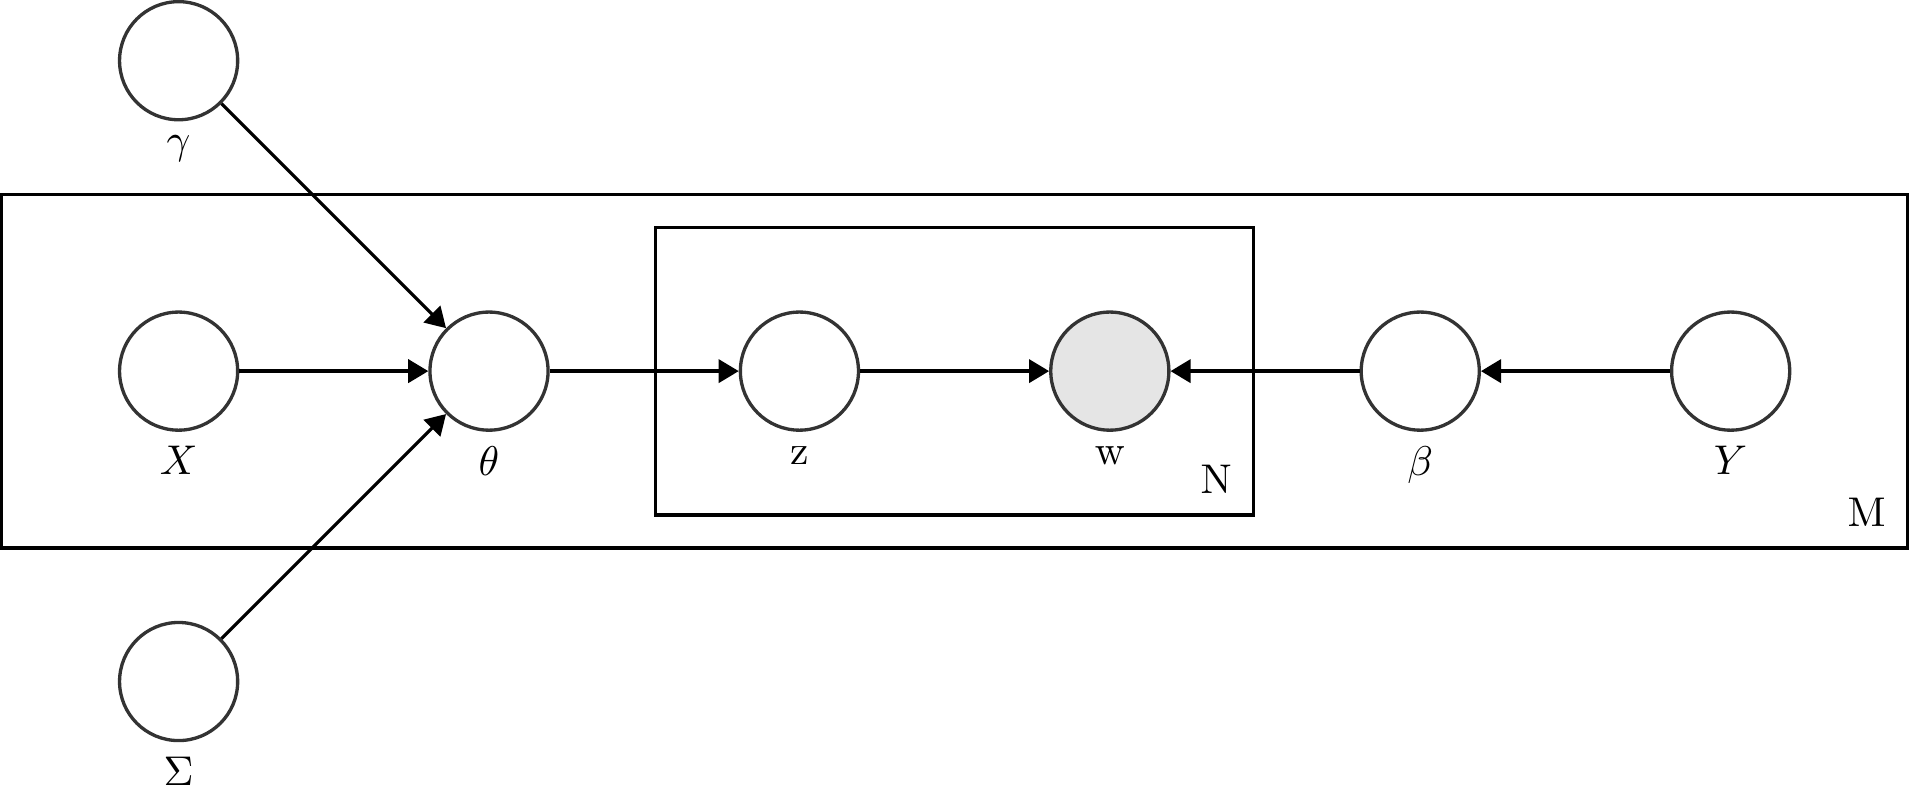
\includegraphics[width=0.9\linewidth]{_main_files/figure-latex/stm-diagram-1} \caption{Plate diagram for a Structucal Topic Model.}(\#fig:stm-diagram)
\end{figure}

\hfill\break

Figure @ref(fig:stm-diagram) shows stm in the form of a plate diagram. Here, \(X\) refers to the prevalence metadata; \(\gamma\), the metadata weights; \(\Sigma\), the topic covariances; \(\theta\), the document prevalence; \(z\), the per-word topic; \(w\), the observed word; \(Y\), the content metadata; \(\beta\), the topic content; \(N\), the number of words in a document; and \(M\), the number of documents in the corpus.

To run stm in R, we have to load the package, set a seed, convert our dfm to the stm format and place our documents, vocabulary (the tokens) and any other data in three separate objects (for later convenience):

\begin{Shaded}
\begin{Highlighting}[]
\FunctionTok{library}\NormalTok{(stm)}
\FunctionTok{library}\NormalTok{(quanteda)}

\FunctionTok{set.seed}\NormalTok{(}\DecValTok{42}\NormalTok{)}

\NormalTok{data\_inaugural\_stm }\OtherTok{\textless{}{-}} \FunctionTok{convert}\NormalTok{(data\_inaugural\_dfm, }\AttributeTok{to =} \StringTok{"stm"}\NormalTok{)}

\NormalTok{documents }\OtherTok{\textless{}{-}}\NormalTok{ data\_inaugural\_stm}\SpecialCharTok{$}\NormalTok{documents}
\NormalTok{vocabulary }\OtherTok{\textless{}{-}}\NormalTok{ data\_inaugural\_stm}\SpecialCharTok{$}\NormalTok{vocab}
\NormalTok{meta }\OtherTok{\textless{}{-}}\NormalTok{ data\_inaugural\_stm}\SpecialCharTok{$}\NormalTok{meta}
\end{Highlighting}
\end{Shaded}

The first thing we have to do is find the number of topics we need. In the \texttt{stm} package, we can do this by using a function called \texttt{searchK}. Here, we specify a range of values that could include the `correct' number of topics, which we then run and collect. Afterwards, we then look at several goodness-of-fit measures to assess which number of topics (which \emph{k}) has the best fit for the data. These measures include exclusivity, semantic coherence, held-out likelihood, bound, lbound, and residual dispersion. Here, we run this for 2 to 15 possible topics.

In our code, we specify our documents, our tokens (the vocabulary), and our meta-data. Moreover, as our prevalence, we include parameters for \texttt{Year} and \texttt{Party}, as we expect the content of the topics to differ between both the Republican and Democratic party, as well as over time:

\begin{Shaded}
\begin{Highlighting}[]
\NormalTok{k }\OtherTok{\textless{}{-}} \FunctionTok{c}\NormalTok{(}\DecValTok{3}\NormalTok{,}\DecValTok{4}\NormalTok{,}\DecValTok{5}\NormalTok{,}\DecValTok{6}\NormalTok{,}\DecValTok{7}\NormalTok{,}\DecValTok{8}\NormalTok{,}\DecValTok{9}\NormalTok{,}\DecValTok{10}\NormalTok{,}\DecValTok{11}\NormalTok{,}\DecValTok{12}\NormalTok{,}\DecValTok{13}\NormalTok{,}\DecValTok{14}\NormalTok{,}\DecValTok{15}\NormalTok{)}
\end{Highlighting}
\end{Shaded}

\begin{Shaded}
\begin{Highlighting}[]
\NormalTok{findingk }\OtherTok{\textless{}{-}} \FunctionTok{searchK}\NormalTok{(documents, vocabulary, k, }\AttributeTok{prevalence =}\SpecialCharTok{\textasciitilde{}}\NormalTok{ Party }\SpecialCharTok{+} \FunctionTok{s}\NormalTok{(Year), }\AttributeTok{data =}\NormalTok{ meta, }\AttributeTok{verbose=}\ConstantTok{TRUE}\NormalTok{)}
\end{Highlighting}
\end{Shaded}

\begin{Shaded}
\begin{Highlighting}[]
\NormalTok{findingk\_results }\OtherTok{\textless{}{-}} \FunctionTok{as.data.frame}\NormalTok{(}\FunctionTok{matrix}\NormalTok{(}\FunctionTok{unlist}\NormalTok{(findingk}\SpecialCharTok{$}\NormalTok{results), }\AttributeTok{nrow=}\FunctionTok{length}\NormalTok{(}\FunctionTok{unlist}\NormalTok{(findingk}\SpecialCharTok{$}\NormalTok{results[}\DecValTok{1}\NormalTok{]))))}
\NormalTok{names }\OtherTok{\textless{}{-}} \FunctionTok{names}\NormalTok{(findingk}\SpecialCharTok{$}\NormalTok{results)}
\FunctionTok{names}\NormalTok{(findingk\_results) }\OtherTok{\textless{}{-}}\NormalTok{ names}
\end{Highlighting}
\end{Shaded}

Looking at \texttt{findingk\_results} we find various values. The first, exclusivity, refers to the occurrence that when words have a high probability under one topic, they have a low probability under others. Related to this is semantic coherence which happens when the most probable words in a topic should occur in the same document. Held-out (or held-out log-likelihood) is the likelihood of our model on data that was not used in the initial estimation (the lower the better), while residuals refer to the difference between a data point and the mean value that the model predicts for that data point (which we want to be 1, indicating a standard distribution). Finally, bound and lbound refer to a model's internal measure of fit. Here, we will be looking for the number of topics, that balance the exclusivity and the semantic coherence, have a residual around 1, and a low held-out. To make this simpler, we visualise our data. In the first graph we plot all the values, while in the second, we only look at the exclusivity and the semantic coherence (as they are the most important):

\begin{Shaded}
\begin{Highlighting}[]
\FunctionTok{library}\NormalTok{(reshape2)}

\NormalTok{findingk\_melt }\OtherTok{\textless{}{-}} \FunctionTok{melt}\NormalTok{(findingk\_results, }\AttributeTok{id=}\StringTok{"K"}\NormalTok{) }
\NormalTok{findingk\_melt}\SpecialCharTok{$}\NormalTok{variable }\OtherTok{\textless{}{-}} \FunctionTok{as.character}\NormalTok{(findingk\_melt}\SpecialCharTok{$}\NormalTok{variable)}
\NormalTok{findingk}\SpecialCharTok{$}\NormalTok{K }\OtherTok{\textless{}{-}} \FunctionTok{as.factor}\NormalTok{(findingk\_results}\SpecialCharTok{$}\NormalTok{K)}

\FunctionTok{ggplot}\NormalTok{(findingk\_melt, }\FunctionTok{aes}\NormalTok{(K, value)) }\SpecialCharTok{+}
 \FunctionTok{geom\_point}\NormalTok{()}\SpecialCharTok{+}
 \FunctionTok{geom\_line}\NormalTok{()}\SpecialCharTok{+}
 \FunctionTok{facet\_wrap}\NormalTok{(}\SpecialCharTok{\textasciitilde{}}\NormalTok{ variable, }\AttributeTok{scales =} \StringTok{"free"}\NormalTok{)}\SpecialCharTok{+}
 \FunctionTok{theme\_classic}\NormalTok{()}
\end{Highlighting}
\end{Shaded}

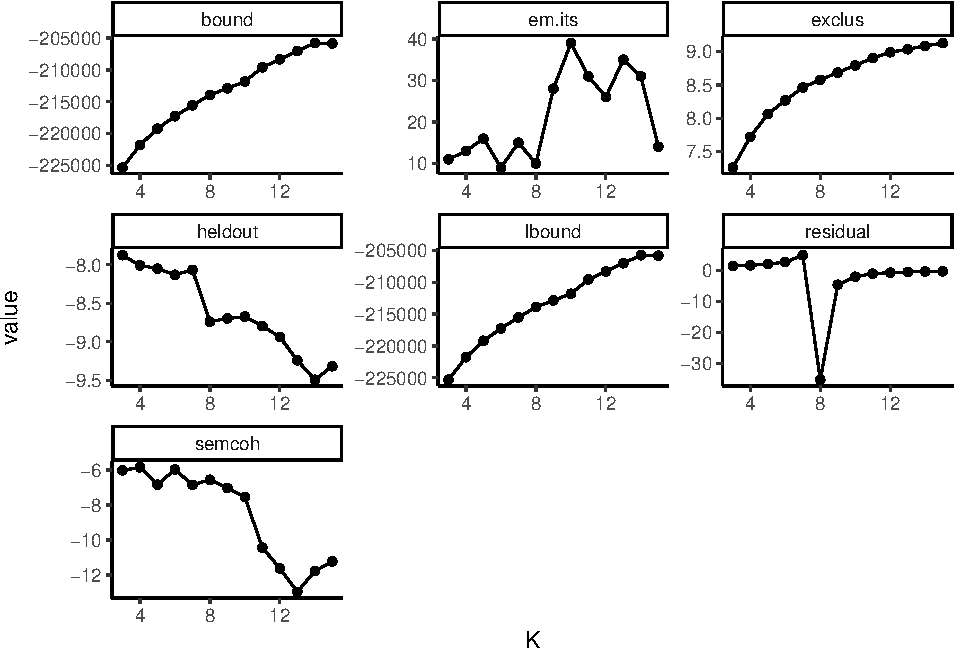
\includegraphics{_main_files/figure-latex/ggplot-stm-findk-1.pdf}

\begin{Shaded}
\begin{Highlighting}[]
\FunctionTok{ggplot}\NormalTok{(findingk\_results, }\FunctionTok{aes}\NormalTok{(semcoh, exclus)) }\SpecialCharTok{+}
 \FunctionTok{geom\_point}\NormalTok{()}\SpecialCharTok{+}
 \FunctionTok{geom\_text}\NormalTok{(}\AttributeTok{data=}\NormalTok{findingk\_results, }\AttributeTok{label=}\NormalTok{findingk}\SpecialCharTok{$}\NormalTok{K, }\AttributeTok{nudge\_x =} \FloatTok{0.15}\NormalTok{)}\SpecialCharTok{+}
 \FunctionTok{scale\_x\_continuous}\NormalTok{(}\StringTok{"Semantic Coherence"}\NormalTok{)}\SpecialCharTok{+}
 \FunctionTok{scale\_y\_continuous}\NormalTok{(}\StringTok{"Exclusivity"}\NormalTok{)}\SpecialCharTok{+}
 \FunctionTok{theme\_classic}\NormalTok{()}
\end{Highlighting}
\end{Shaded}

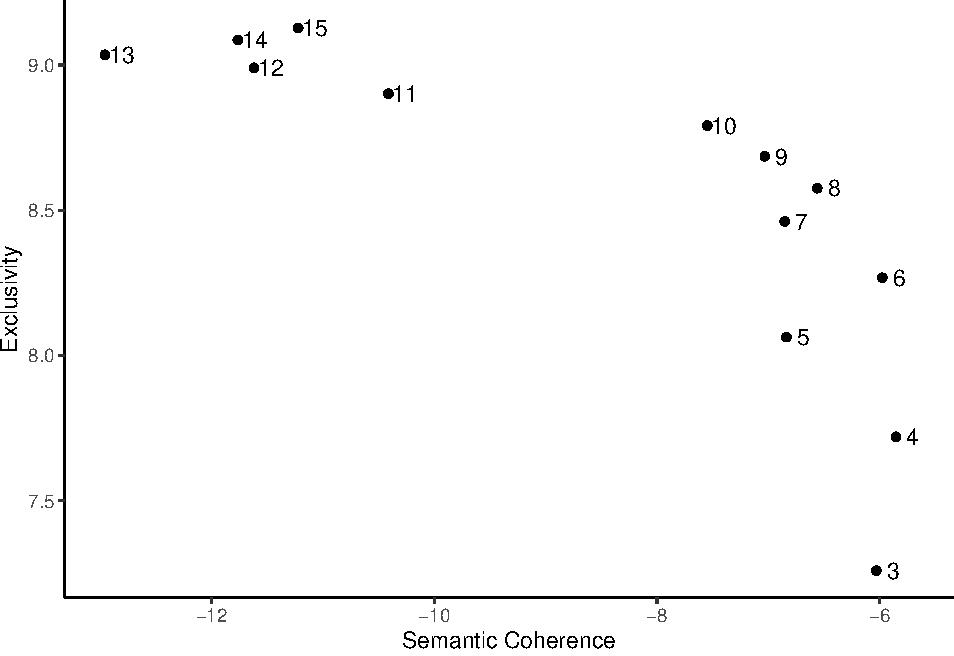
\includegraphics{_main_files/figure-latex/ggplot-stm-findk-2.pdf}

Based on these graphs, we decide upon 8 topics. The main reason for this is that for this number of topics, there is a high semantic coherence given the exclusivity. We can now run our stm model, using spectral initialization and a topical prevalence including both the Party and the Year of the inauguration. Also, we have a look at the topics, and the words with the highest probability attached to them:

\begin{Shaded}
\begin{Highlighting}[]
\NormalTok{n\_topics }\OtherTok{\textless{}{-}} \DecValTok{8}
\NormalTok{output\_stm }\OtherTok{\textless{}{-}} \FunctionTok{stm}\NormalTok{(documents, vocabulary, }\AttributeTok{K =}\NormalTok{ n\_topics, }\AttributeTok{prevalence =}\SpecialCharTok{\textasciitilde{}}\NormalTok{ Party }\SpecialCharTok{+} \FunctionTok{s}\NormalTok{(Year), }\AttributeTok{data =}\NormalTok{ meta, }\AttributeTok{init.type =} \StringTok{"Spectral"}\NormalTok{, }\AttributeTok{verbose=}\ConstantTok{TRUE}\NormalTok{)}
\end{Highlighting}
\end{Shaded}

\begin{Shaded}
\begin{Highlighting}[]
\FunctionTok{labelTopics}\NormalTok{(output\_stm)}
\end{Highlighting}
\end{Shaded}

\begin{verbatim}
## Topic 1 Top Words:
##       Highest Prob: free, peace, world, shall, freedom, must, faith 
##       FREX: strive, free, peoples, everywhere, truth, man's, learned 
##       Lift: abhorring, absorbing, abstractions, acquire, aggressor, amass, andes 
##       Score: anguished, productivity, strive, trial, learned, europe, defines 
## Topic 2 Top Words:
##       Highest Prob: us, new, world, let, can, people, america 
##       FREX: let, century, together, new, weapons, voices, abroad 
##       Lift: 200th, 20th, dawn, explore, micah, moon, music 
##       Score: attempting, nuclear, let, celebrate, voices, abroad, dawn 
## Topic 3 Top Words:
##       Highest Prob: us, must, world, government, people, america, can 
##       FREX: civilization, republic, experiment, normal, relationship, order, industrial 
##       Lift: deliberate, inspiration, intention, regards, tremendous, unshaken, abnormal 
##       Score: accompanied, supreme, regards, deliberate, inspiration, unshaken, righteousness 
## Topic 4 Top Words:
##       Highest Prob: us, america, nation, can, must, new, people 
##       FREX: story, thank, president, defend, everyone, children, america 
##       Lift: breeze, january, accounting, accumulate, activism, addiction, agitate 
##       Score: allowing, story, breeze, talk, crucial, everyone, virus 
## Topic 5 Top Words:
##       Highest Prob: freedom, nation, people, america, government, know, democracy 
##       FREX: speaks, mind, democracy, liberty, seen, came, millions 
##       Lift: paint, abreast, absence, admiration, agent, amount, aspires 
##       Score: charta, speaks, paint, disaster, mind, defended, seen 
## Topic 6 Top Words:
##       Highest Prob: us, must, nation, people, can, new, every 
##       FREX: generation, journey, union, change, covenant, creed, enduring 
##       Lift: demanded, mastery, span, storms, absolutism, abundantly, afghanistan 
##       Score: abundantly, covenant, journey, mastery, storms, demanded, span 
## Topic 7 Top Words:
##       Highest Prob: can, world, people, peace, nations, must, government 
##       FREX: settlement, enforcement, countries, desire, party, international, property 
##       Lift: abound, absurd, acceptance, accepts, accordingly, accountability, accounted 
##       Score: abound, enforcement, contributed, settlement, property, major, eighteenth 
## Topic 8 Top Words:
##       Highest Prob: upon, government, shall, can, must, great, may 
##       FREX: army, interstate, negro, executive, tariff, business, proper 
##       Lift: affected, amendments, antitrust, army, attention, avail, banking 
##       Score: tariff, interstate, army, negro, policy, proper, business
\end{verbatim}

Here, we see that the word \texttt{us} is dominant in most topics, making it a candidate for removal as a stop word in a future analysis. Looking closer, we find that the first topic refers to peace, the second, third and seventh to the world, the fourth and sixth to America, and the eighth to the government.

Finally, we can see whether there is any relation between these topics and any of the parameters we included. Here, let us look at any existing differences between the two parties:

\begin{Shaded}
\begin{Highlighting}[]
\NormalTok{est\_assoc\_effect }\OtherTok{\textless{}{-}} \FunctionTok{estimateEffect}\NormalTok{(}\SpecialCharTok{\textasciitilde{}}\NormalTok{Party, output\_stm, }\AttributeTok{metadata =}\NormalTok{ meta, }\AttributeTok{prior=}\FloatTok{1e{-}5}\NormalTok{)}
\end{Highlighting}
\end{Shaded}

While we can visualise this with the \texttt{plot.estimateEffect} option, the visualisation is far from ideal. Thus, let us use some data-wrangling and make the plot ourselves:

\begin{Shaded}
\begin{Highlighting}[]
\NormalTok{estimate\_data }\OtherTok{\textless{}{-}} \FunctionTok{plot.estimateEffect}\NormalTok{(est\_assoc\_effect, }\StringTok{"Party"}\NormalTok{, }\AttributeTok{method =} \StringTok{"pointestimate"}\NormalTok{, }\AttributeTok{model =}\NormalTok{ output\_stm, }\AttributeTok{omit.plot =} \ConstantTok{TRUE}\NormalTok{)}
\NormalTok{estimate\_graph\_means }\OtherTok{\textless{}{-}}\NormalTok{ estimate\_data}\SpecialCharTok{$}\NormalTok{means}
\NormalTok{estimate\_graph\_means }\OtherTok{\textless{}{-}} \FunctionTok{data.frame}\NormalTok{(}\FunctionTok{matrix}\NormalTok{(}\FunctionTok{unlist}\NormalTok{(estimate\_graph\_means), }\AttributeTok{nrow=}\FunctionTok{length}\NormalTok{(estimate\_graph\_means), }\AttributeTok{byrow=}\ConstantTok{TRUE}\NormalTok{))}
\NormalTok{estimate\_graph\_means }\OtherTok{\textless{}{-}} \FunctionTok{data.frame}\NormalTok{(}\FunctionTok{c}\NormalTok{(}\FunctionTok{rep}\NormalTok{(}\StringTok{"Republicans"}\NormalTok{, }\DecValTok{8}\NormalTok{), }\FunctionTok{rep}\NormalTok{(}\StringTok{"Democrats"}\NormalTok{, }\DecValTok{8}\NormalTok{)), }\FunctionTok{c}\NormalTok{(estimate\_graph\_means}\SpecialCharTok{$}\NormalTok{X1,estimate\_graph\_means}\SpecialCharTok{$}\NormalTok{X2))}

\NormalTok{estimate\_graph\_cis }\OtherTok{\textless{}{-}}\NormalTok{ estimate\_data}\SpecialCharTok{$}\NormalTok{cis}
\NormalTok{estimate\_graph\_cis }\OtherTok{\textless{}{-}} \FunctionTok{data.frame}\NormalTok{(}\FunctionTok{matrix}\NormalTok{(}\FunctionTok{unlist}\NormalTok{(estimate\_graph\_cis), }\AttributeTok{nrow=}\FunctionTok{length}\NormalTok{(estimate\_graph\_cis), }\AttributeTok{byrow=}\ConstantTok{TRUE}\NormalTok{))}
\NormalTok{estimate\_graph\_cis }\OtherTok{\textless{}{-}} \FunctionTok{data.frame}\NormalTok{(}\FunctionTok{c}\NormalTok{(estimate\_graph\_cis}\SpecialCharTok{$}\NormalTok{X1,estimate\_graph\_cis}\SpecialCharTok{$}\NormalTok{X3), }\FunctionTok{c}\NormalTok{(estimate\_graph\_cis}\SpecialCharTok{$}\NormalTok{X2,estimate\_graph\_cis}\SpecialCharTok{$}\NormalTok{X4))}

\NormalTok{Topic }\OtherTok{\textless{}{-}} \FunctionTok{c}\NormalTok{(}\StringTok{"Topic 1"}\NormalTok{, }\StringTok{"Topic 2"}\NormalTok{, }\StringTok{"Topic 3"}\NormalTok{, }\StringTok{"Topic 4"}\NormalTok{,}\StringTok{"Topic 5"}\NormalTok{, }\StringTok{"Topic 6"}\NormalTok{, }\StringTok{"Topic 7"}\NormalTok{, }\StringTok{"Topic 8"}\NormalTok{, }\StringTok{"Topic 1"}\NormalTok{, }\StringTok{"Topic 2"}\NormalTok{, }\StringTok{"Topic 3"}\NormalTok{, }\StringTok{"Topic 4"}\NormalTok{,}\StringTok{"Topic 5"}\NormalTok{, }\StringTok{"Topic 6"}\NormalTok{, }\StringTok{"Topic 7"}\NormalTok{, }\StringTok{"Topic 8"}\NormalTok{)}

\NormalTok{estimate\_graph }\OtherTok{\textless{}{-}} \FunctionTok{cbind}\NormalTok{(Topic, estimate\_graph\_means,estimate\_graph\_cis)}
\FunctionTok{names}\NormalTok{(estimate\_graph) }\OtherTok{\textless{}{-}} \FunctionTok{c}\NormalTok{(}\StringTok{"Topic"}\NormalTok{,}\StringTok{"Party"}\NormalTok{,}\StringTok{"Mean"}\NormalTok{, }\StringTok{"min"}\NormalTok{, }\StringTok{"max"}\NormalTok{)}
\NormalTok{estimate\_graph}\SpecialCharTok{$}\NormalTok{Party }\OtherTok{\textless{}{-}} \FunctionTok{as.factor}\NormalTok{(estimate\_graph}\SpecialCharTok{$}\NormalTok{Party)}
\NormalTok{estimate\_graph}\SpecialCharTok{$}\NormalTok{Topic }\OtherTok{\textless{}{-}} \FunctionTok{as.factor}\NormalTok{(estimate\_graph}\SpecialCharTok{$}\NormalTok{Topic)}
\NormalTok{estimate\_graph}\SpecialCharTok{$}\NormalTok{Topic }\OtherTok{\textless{}{-}} \FunctionTok{factor}\NormalTok{(estimate\_graph}\SpecialCharTok{$}\NormalTok{Topic, }\AttributeTok{levels=}\FunctionTok{rev}\NormalTok{(}\FunctionTok{levels}\NormalTok{(estimate\_graph}\SpecialCharTok{$}\NormalTok{Topic)))}
\end{Highlighting}
\end{Shaded}

Now, let us plot our intervals:

\begin{Shaded}
\begin{Highlighting}[]
\FunctionTok{ggplot}\NormalTok{(estimate\_graph, }\FunctionTok{aes}\NormalTok{(Mean, Topic)) }\SpecialCharTok{+}
 \FunctionTok{geom\_pointrange}\NormalTok{(}\FunctionTok{aes}\NormalTok{(}\AttributeTok{xmin =}\NormalTok{ min, }\AttributeTok{xmax =}\NormalTok{ max, }\AttributeTok{color =}\NormalTok{ Party),}
                 \AttributeTok{position =} \FunctionTok{position\_dodge}\NormalTok{(}\FloatTok{0.3}\NormalTok{))}\SpecialCharTok{+}
 \FunctionTok{geom\_vline}\NormalTok{(}\AttributeTok{xintercept =} \DecValTok{0}\NormalTok{,}
            \AttributeTok{linetype=}\StringTok{"dashed"}\NormalTok{, }\AttributeTok{size=}\FloatTok{0.5}\NormalTok{)}\SpecialCharTok{+}
 \FunctionTok{scale\_color\_manual}\NormalTok{(}\AttributeTok{values =} \FunctionTok{c}\NormalTok{(}\StringTok{"\#0015BC"}\NormalTok{, }\StringTok{"\#E9141D"}\NormalTok{))}\SpecialCharTok{+}
 \FunctionTok{theme\_classic}\NormalTok{()}
\end{Highlighting}
\end{Shaded}

\begin{verbatim}
## Warning: Using `size` aesthetic for lines was deprecated in ggplot2 3.4.0.
## i Please use `linewidth` instead.
## This warning is displayed once every 8 hours.
## Call `lifecycle::last_lifecycle_warnings()` to see where this warning was
## generated.
\end{verbatim}

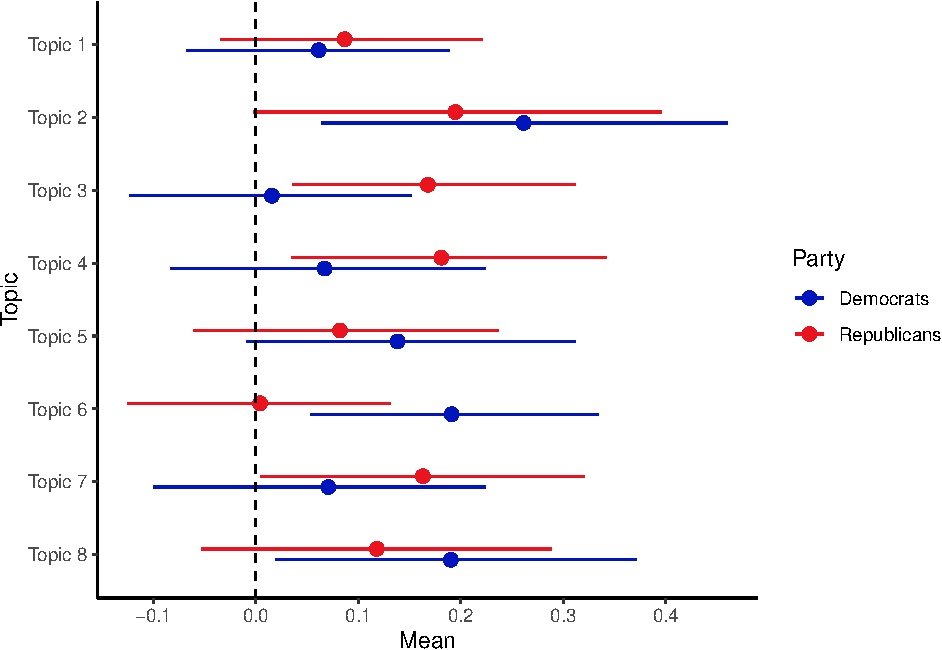
\includegraphics{_main_files/figure-latex/ggplot-stm-intervals-1.pdf}

Here, we find that while the averages for the topic do seem to differ a little between both of the parties, all the intervals are overlapping, indicating that they are not that different.

\chapter{Texttricks}\label{texttricks}

One of the main advantages of using R for quantitative text analysis is that it is (for a part) a general-purpose language. That is, we are not limited to any of the functions that the original designers chose to implement with it. Indeed, this is the reason for the existence of the all the packages we have been using. Indeed, writing a package in R is relatively simple, as is hosting your package and making it available to others.

The main logic of R packages rests on the idea of \emph{functions}. We already saw an example of a function in Chapter @ref(importing-data), where we specified a function to read in a .pdf file and convert it to a .txt file. The way a function in R works it that you encapsulate the commands you require within the \texttt{function} command. Anything between the curly brackets will be treated as part of the function, while everything between the parentheses will be treated as the input of our function.

\begin{Shaded}
\begin{Highlighting}[]
\NormalTok{extract\_pdf }\OtherTok{\textless{}{-}} \ControlFlowTok{function}\NormalTok{(filename) \{}
  \FunctionTok{require}\NormalTok{(pdftools)}
  \FunctionTok{print}\NormalTok{(filename)}
  \FunctionTok{try}\NormalTok{(\{}
\NormalTok{    text }\OtherTok{\textless{}{-}} \FunctionTok{pdf\_text}\NormalTok{(filename)}
\NormalTok{  \})}
\NormalTok{  title }\OtherTok{\textless{}{-}} \FunctionTok{gsub}\NormalTok{(}\StringTok{"(.*)/([\^{}/]*).pdf"}\NormalTok{, }\StringTok{"}\SpecialCharTok{\textbackslash{}\textbackslash{}}\StringTok{2"}\NormalTok{, filename)}
\NormalTok{  txt\_directory }\OtherTok{\textless{}{-}} \FunctionTok{getwd}\NormalTok{()}
  \FunctionTok{write}\NormalTok{(text, }\FunctionTok{file.path}\NormalTok{(txt\_directory, }\FunctionTok{paste0}\NormalTok{(title, }\StringTok{".txt"}\NormalTok{)))}
\NormalTok{\}}
\end{Highlighting}
\end{Shaded}

\begin{itemize}
\tightlist
\item
  \emph{Function Name} - The name of the function and what we need to type into the console in order to run the function
\item
  \emph{Arguments} - Arguments are placeholders. In our case, \texttt{filename} is an argument. This can be anything, and in our case it is the address of where our .pdf file is stored. When we run the function, anything we specify in the place of \texttt{filename} will be treated as such by R.
\item
  \emph{Body} - Everything between the curly brackets that makes up the complete function
\item
  \emph{Return Value} - The output of the function. Can be specified by \texttt{return(value)}. Yet, in our case the return is in the \texttt{write()} command that writes the .txt file to our \texttt{txt\_directory} folder.
\end{itemize}

Compiling this function (or many different functions) into a package, requires a little bit more work, but not much. A very nice introduction is given by \href{https://hilaryparker.com/2014/04/29/writing-an-r-package-from-scratch/}{Hilary Parker}. Here, we placed the function above in the \texttt{texttricks} package. As this package is on GitHub, you can have a look at all its files at: \url{https://github.com/SCJBruinsma/texttricks}.

To install the package within \texttt{R}, use the \texttt{install\_github} command that is part of the devtools package:

\begin{Shaded}
\begin{Highlighting}[]
\FunctionTok{install.packages}\NormalTok{(}\StringTok{"devtools"}\NormalTok{)}
\FunctionTok{library}\NormalTok{(devtools)}
\NormalTok{devtools}\SpecialCharTok{::}\FunctionTok{install\_github}\NormalTok{(}\StringTok{"SCJBruinsma/texttricks"}\NormalTok{)}
\end{Highlighting}
\end{Shaded}

\phantomsection\label{refs}
\begin{CSLReferences}{1}{2}
\bibitem[\citeproctext]{ref-Albaugh2013a}
Albaugh, Q., Sevenans, J., Soroka, S., \& Loewen, P. J. (2013). {The Automated Coding of Policy Agendas: A Dictionary-based Approach}. \emph{6th Annual Comparative Agendas Conference, Antwerp, Belgium}.

\bibitem[\citeproctext]{ref-Bakker2012a}
Bakker, R., Vries, C. de, Edwards, E., Hooghe, L., Jolly, S., Marks, G., Polk, J., Rovny, J., Steenbergen, M. R., \& Vachudova, M. A. (2012). Measuring party positions in europe: The chapel hill expert survey trend file, 1999-2010. \emph{Party Politics}, \emph{21}(1), 1--15. \url{https://doi.org/10.1177/1354068812462931}

\bibitem[\citeproctext]{ref-Benoit2009a}
Benoit, K., Laver, M., \& Mikhaylov, S. (2009). Treating words as data with error: Uncertainty in text statements of policy positions. \emph{American Journal of Political Science}, \emph{53}(2), 495--513. \url{https://doi.org/10.1111/j.1540-5907.2009.00383.x}

\bibitem[\citeproctext]{ref-Benoit2018a}
Benoit, K., Watanabe, K., Wang, H., Nulty, P., Obeng, A., Müller, S., \& Matsuo, A. (2018). Quanteda: An r package for the quantitative analysis of textual data. \emph{Journal of Open Source Software}, \emph{3}(30), 774. \url{https://doi.org/10.21105/joss.00774}

\bibitem[\citeproctext]{ref-Blei2003a}
Blei, D. M., Ng, A. Y., \& Jordan, M. I. (2003). Latent dirichlet allocation. \emph{Journal of Machine Learning Research}, \emph{3}(Jan), 993--1022.

\bibitem[\citeproctext]{ref-Bruns2019a}
Bruns, A. (2019). After the `{API}calypse': Social media platforms and their fight against critical scholarly research. \emph{Information, Communication \& Society}, \emph{22}(11), 1544--1566. \url{https://doi.org/10.1080/1369118X.2019.1637447}

\bibitem[\citeproctext]{ref-Carmines1979a}
Carmines, E. G., \& Zeller, R. A. (1979). \emph{Reliability and validity assessment}. Sage. \url{https://doi.org/10.4135/9781412985642}

\bibitem[\citeproctext]{ref-Clarke2019a}
Clarke, I., \& Grieve, J. (2019). Stylistic variation on the donald trump twitter account: A linguistic analysis of tweets posted between 2009 and 2018. \emph{PLOS ONE}, \emph{14}(9), 1--27. \url{https://doi.org/10.1371/journal.pone.0222062}

\bibitem[\citeproctext]{ref-Freelon2018a}
Freelon, D. (2018). {Computational Research in the Post-API Age}. \emph{Political Communication}, \emph{35}(4), 665--668. \url{https://doi.org/10.1080/10584609.2018.1477506}

\bibitem[\citeproctext]{ref-Griffiths2004a}
Griffiths, T. L., \& Steyvers, M. (2004). Finding scientific topics. \emph{Proceedings of the National Academy of Sciences}, \emph{101}(suppl 1), 5228--5235. \url{https://doi.org/10.1073/pnas.0307752101}

\bibitem[\citeproctext]{ref-Grimmer2022a}
Grimmer, J., Roberts, M. E., \& Stewart, B. M. (2022). \emph{{Text as Data: A New Framework for Machine Learning and the Social Sciences}}. Princeton University Press.

\bibitem[\citeproctext]{ref-Grimmer2013a}
Grimmer, J., \& Stewart, B. M. (2013). Text as data: The promise and pitfals of automatic content analysis methods for political texts. \emph{Political Analysis}, \emph{21}(3), 267--297. \url{https://doi.org/10.1093/pan/mps028}

\bibitem[\citeproctext]{ref-Haselmayer2017a}
Haselmayer, M., \& Jenny, M. (2017). Sentiment analysis of political communication: Combining a dictionary approach with crowdcoding. \emph{Quality \& Quantity}, \emph{51}(6), 2623--2646. \url{https://doi.org/10.1007/s11135-016-0412-4}

\bibitem[\citeproctext]{ref-Hayes2007a}
Hayes, A. F., \& Krippendorff, K. (2007). Answering the call for a standard reliability measure for coding data. \emph{Communication Methods and Measures}, \emph{1}(1), 77--89. \url{https://doi.org/10.1080/19312450709336664}

\bibitem[\citeproctext]{ref-Hutto2014a}
Hutto, C., \& Gilbert, E. (2014). VADER: A parsimonious rule-based model for sentiment analysis of social media text. \emph{Proceedings of the International AAAI Conference on Web and Social Media}, \emph{8}(1), 216--225. \url{https://doi.org/10.1609/icwsm.v8i1.14550}

\bibitem[\citeproctext]{ref-Krippendorff2004a}
Krippendorff, K. (2018). \emph{{Content Analysis - an Introduction to Its Methodology}} (4th ed.). Sage.

\bibitem[\citeproctext]{ref-Lamprianou2020a}
Lamprianou, I. (2020). Measuring and visualizing coders' reliability: New approaches and guidelines from experimental data. \emph{Sociological Methods \& Research}. \url{https://doi.org/10.1177/0049124120926198}

\bibitem[\citeproctext]{ref-Laver2003a}
Laver, M., Benoit, K., \& Garry, J. (2003). Extracting policy positions from political texts using words as data. \emph{The American Political Science Review}, \emph{97}(2), 311--331. \url{https://doi.org/10.1017/S0003055403000698}

\bibitem[\citeproctext]{ref-Laver2000a}
Laver, M., \& Garry, J. (2000). Estimating policy positions from political texts. \emph{American Journal of Political Science}, \emph{44}(3), 619--634. \url{https://doi.org/10.2307/2669268}

\bibitem[\citeproctext]{ref-Le2008a}
Lê, S., Josse, J., \& Husson, F. (2008). Factominer: An r package for multivariate analysis. \emph{Journal of Statistical Software}, \emph{25}(1). \url{https://doi.org/10.18637/jss.v025.i01}

\bibitem[\citeproctext]{ref-Lin1989a}
Lin, L. (1989). A concordance correlation coefficient to evaluate reproducibility. \emph{Biometrics}, \emph{45}, 255--268. \url{https://doi.org/10.2307/2532051}

\bibitem[\citeproctext]{ref-Lind2019a}
Lind, F., Eberl, J.-M., Heidenreich, T., \& Boomgaarden, H. G. (2019). When the journey is as important as the goal: A roadmap to multilingual dictionary construction. \emph{International Journal of Communication}, \emph{13}, 4000--4020.

\bibitem[\citeproctext]{ref-Lowe2011b}
Lowe, W. (2011). \emph{{JFreq: Count Words, Quickly}}. \url{http://www.conjugateprior.org/software/jfreq/}

\bibitem[\citeproctext]{ref-Lowe2011a}
Lowe, W., \& Benoit, K. (2011). Estimating uncertainty in quantitative text analysis. \emph{Annual Meeting of the Midwest Political Science Association}.

\bibitem[\citeproctext]{ref-Martin2008a}
Martin, L. W., \& Vanberg, G. (2008). Reply to benoit and laver. \emph{Political Analysis}, \emph{16}(1), 112--114. \url{https://doi.org/10.1093/pan/mpm018}

\bibitem[\citeproctext]{ref-Merz2016a}
Merz, N., Regel, S., \& Lewandowski, J. (2016). The manifesto corpus: A new resource for research on political parties and quantitative text analysis. \emph{Research \& Politics}, \emph{3}(2), 2053168016643346. \url{https://doi.org/10.1177/2053168016643346}

\bibitem[\citeproctext]{ref-Mikhaylov2012a}
Mikhaylov, S., Laver, M., \& Benoit, K. (2012). Coder reliability and misclassification in the human coding of party manifestos. \emph{Political Analysis}, \emph{20}(1), 78--91. \url{https://doi.org/10.1093/pan/mpr047}

\bibitem[\citeproctext]{ref-Munzert2014a}
Munzert, S., Rubba, C., Meißner, P., \& Nyhuis, D. (2014). \emph{Automated data collection with r: A practical guide to web scraping and text mining}. John Wiley \& Sons.

\bibitem[\citeproctext]{ref-Perriam2020a}
Perriam, J., Birkbak, A., \& Freeman, A. (2020). {Digital Methods in a Post-API Environment}. \emph{International Journal of Social Research Methodology}, \emph{23}(3), 277--290. \url{https://doi.org/10.1080/13645579.2019.1682840}

\bibitem[\citeproctext]{ref-Roberts2019a}
Roberts, M. E., Stewart, B. M., \& Tingley, D. (2019). {stm: An R Package for Structural Topic Models}. \emph{Journal of Statistical Software}, \emph{91}(2). \url{https://doi.org/10.18637/jss.v091.i02}

\bibitem[\citeproctext]{ref-Roberts2014a}
Roberts, M. E., Stewart, B. M., Tingley, D., Lucas, C., Leder-Luis, J., Gadarian, S. K., Albertson, B., \& Rand, D. G. (2014). Structural topic models for open-ended survey responses. \emph{American Journal of Political Science}, \emph{58}(4), 1064--1082. \url{https://doi.org/10.1111/ajps.12103}

\bibitem[\citeproctext]{ref-Slapin2008a}
Slapin, J. B., \& Proksch, S.-O. (2008). A scaling model for estimating time-series party positions from texts. \emph{American Journal of Political Science}, \emph{52}(3), 705--722. \url{https://doi.org/10.1111/j.1540-5907.2008.00338.x}

\bibitem[\citeproctext]{ref-Volkens2019a}
Volkens, A., Krause, W., Lehmann, P., Matthieß, T., Merz, N., Regel, S., \& Weßels, B. (2019). \emph{{The Manifesto Data Collection. Manifesto Project (MRG/CMP/MARPOR)}}. Berlin: Wissenschaftszentrum Berlin f{ü}r Sozialforschung (WZB). \url{https://doi.org/10.25522/manifesto.mpds.2019b}

\bibitem[\citeproctext]{ref-Welbers2017a}
Welbers, K., Van Atteveldt, W., \& Benoit, K. (2017). {Text Analysis in R}. \emph{Communication Methods and Measures}, \emph{11}(4), 245--265. \url{https://doi.org/10.1080/19312458.2017.1387238}

\bibitem[\citeproctext]{ref-Young2012a}
Young, L., \& Soroka, S. (2012). \emph{Lexicoder sentiment dictionary}. \url{http://www.snsoroka.com/data-lexicoder/}

\end{CSLReferences}

\end{document}
